\documentclass[titlepage,a4paper,openany]{report}
\usepackage[latin1]{inputenc}
\usepackage{stmaryrd} % For boxy Maths symbols
\usepackage{wasysym} % for circly Maths symbols
\usepackage{epsdice} % for dice symbols
\usepackage{appendix}
\usepackage{geometry}
\usepackage{array}
\usepackage{svg}
\usepackage{alltt}
\svgsetup{width=\textwidth}
\usepackage{tabularx}
\usepackage{wrapfig}
\usepackage{float}
\usepackage{epigraph}
\usepackage{makeidx}
\usepackage[english]{babel}
\usepackage{multicol}
\usepackage{graphicx}
\usepackage{incgraph}
\usepackage{etoolbox}
\usepackage{float}
\usepackage{titlesec}
\usepackage{needspace}
\usepackage{tikz}
\usetikzlibrary{mindmap,trees}
\usepackage{pifont}
\usepackage{colortbl}
\usepackage[poster]{tcolorbox}
\tcbuselibrary{breakable,raster}
\tcbset{enhanced,colback=white,breakable,arc=6mm,outer arc=1mm}

%%%%%%%%%% Section Headers %%%%%%%%%%

%%% Allow quotes under part headers
\makeatletter
\let\old@endpart\@endpart
\renewcommand\@endpart[1][]{%
\begin{quote}#1\end{quote}%
\old@endpart}
\makeatother

\titleformat{\chapter}[frame]
{\normalfont}
{\filright
\footnotesize
\enspace SECTION \thesection\enspace}
{8pt}
{\Huge\filcenter\bfseries}

\newcommand{\chapnumfont}{
  \fontsize{144}{0}
  \selectfont
}

%%%%%%%%%% Encounter Numbers
\newcounter{encnum}
\setcounter{encnum}{1}
\newcommand{\encsymbol}{\ding{168}}
\newcommand{\encnum}{\ifnumcomp{\value{encnum}}{=}{1}{$A$}{\arabic{encnum}}\encsymbol\addtocounter{encnum}{1}}

\newcommand{\headingtype}{CHAPTER}

\newcommand{\sidepic}[2]{
	\needspace{3cm}\begin{wrapfigure}{O}{.#1\textwidth}
\includegraphics[width=.#1\textwidth]{images/#2}
\end{wrapfigure}
}

\colorlet{chapnumcol}{black!55}

\titleformat{\chapter}[display]
{\bfseries}
{
\begin{tikzpicture}
  \node[minimum width=\textwidth, text=black!25, fill=black!25, inner sep=1, outer sep=0, anchor=south] (rectinit) {\huge CHAPTER};
  \node[minimum width=.8\textwidth, text=white, inner sep=1, outer sep=0, anchor=south west, text width=.8\textwidth, align=right] at (rectinit.south west) (chapname) {\huge \headingtype~~};
  \node[minimum width=.2\textwidth, inner sep=0, outer sep=0, anchor=south west, text width=.2\textwidth, align=left] at (chapname.south east) {\chapnumfont\textcolor{chapnumcol}{\thechapter}};
\end{tikzpicture}}
{0pt}
{\Huge}

\titleformat{\section}[frame]
{\needspace{4cm}\normalfont}
{\filright
\footnotesize
\enspace SECTION \thesection\enspace}
{8pt}
{\Large\bfseries\filcenter}

\titleformat{\subsection}{\needspace{4cm}\large\bfseries}{}{1em}{}[\rule{.5\textwidth}{.2pt}]
%
%\titleformat{\section}
%{\needspace{4\textheight}\normalfont\Large\bfseries}{\thesection}
%{1em}
%{
%\vspace{1ex}
%}[\titlerule]
%
%\titleformat{\subsubsection}
%{\normalfont\normalsize\bfseries}{}{1em}{\ding{227} }
%
%\titleformat{\paragraph}[runin]
%{\normalfont\normalsize\bfseries}{\theparagraph}{1em}{}
%
%\titleformat{\subparagraph}[runin]
%{\normalfont\normalsize\bfseries}{\thesubparagraph}{1em}{}

%\titlespacing*{\chapter}
%{0pt}{50pt}{40pt}
%\titlespacing*{\section}
%{0pt}{3.5ex plus 1ex minus .2ex}{2.3ex plus .2ex}
%\titlespacing*{\subsection}
%{0pt}{3.25ex plus 1ex minus .2ex}{1.5ex plus .2ex}
%\titlespacing*{\subsubsection}{0pt}{3.25ex plus 1ex minus .2ex}{1.5ex plus .2ex}
%\titlespacing*{\paragraph}
%{0pt}{3.25ex plus 1ex minus .2ex}{1em}
%\titlespacing*{\subparagraph} {\parindent}{3.25ex plus 1ex minus .2ex}{1em}

%%%%% Character Sheet Tracker

		\newcounter{track}
		\setcounter{track}{18}
		\newcommand{\tracker}{\center\noindent\arabic{track}\addtocounter{track}{-1}\vspace{.54cm}

		}


\newcommand{\character}[1]{\needspace{12em}\vspace{.38cm} \normalsize\bfseries\ding{70} #1 \ding{70}\vspace{.18cm}}

\newcommand{\Character}[3]{\needspace{4em}\vspace{.38cm} \normalsize\bfseries\ding{70} #1 \ding{70}

\hspace{.5cm}\textbf{Personality:} #2

\hspace{.5cm}\textbf{Mannerism:} #3

}

\newcommand{\monster}[1]{\needspace{4em}\vspace{.38cm} \normalsize\bfseries\ding{70} #1 \ding{70}\vspace{.18cm}}

%%%%%%%%%%%%%%%%%%%% TOGGLES %%%%%%%%%%%%%%%%%%%%

\newtoggle{verbose}
\settoggle{verbose}{true}

\iftoggle{verbose}{
	\setcounter{tocdepth}{1}
	\setcounter{secnumdepth}{1}
}

\newcounter{enc}
\newcounter{list}
\newcounter{spelllevel}
\setcounter{spelllevel}{0}


%%%%%%%%%%%%%%%%%%%% LAYOUT %%%%%%%%%%%%%%%%%%%%
\makeindex
\raggedbottom

\newcommand{\currentsphere}{magic}
\newcommand{\sphere}[1]{\setcounter{spelllevel}{0}\renewcommand{\currentsphere}{#1}\index{#1}\section{\currentsphere}}
\newcommand{\spelllevel}{\addtocounter{spelllevel}{1}\subsection{\currentsphere~ Level \arabic{spelllevel}}\noindent}
\newcommand{\enhancement}[2]{\paragraph{(#1) #2:}}

\newcommand{\spell}[3]{\subsubsection{#1}

{\it Type: #2, Skill: #3}

\noindent}

% Toggles for knacks

%%%%%%%%%%%%%%%%%%%% Environments %%%%%%%%%%%%%%%%%%%%
\newenvironment{boxtext}{\begin{quotation}\noindent}{\end{quotation}}

\newenvironment{speechtext}{\begin{quotation}\noindent}{\end{quotation}}

\tcolorboxenvironment{boxtext}{}
\tcolorboxenvironment{speechtext}{}

\newenvironment{rolltable}%
{\vspace{.3cm}\begin{tabular}{|lp{.8\textwidth}}


Roll & Result \\
\hline

}%
{\end{tabular}}


\newenvironment{exampletext}{\needspace{4cm}\vspace{.3cm}

\rule{.9\linewidth}{0.2pt}

\vspace{.3cm}

\it}{\normalfont}

\newtcolorbox{xpchart}[1]{tabularx={l|p{.9\textwidth}},arc=0mm,adjusted title=XP Rewards for #1}

\newtcolorbox[use counter=enc, use counter=list]{encounters}[1]{adjusted title=Encounters in #1,arc=1mm,tabularx={XXp{.7\textwidth}},code={\setcounter{enc}{19}\setcounter{list}{18}}}

\newtcolorbox{rollchart}{tabularx={cp{.84\textwidth}},arc=1mm}

\newtcolorbox{xpbox}[1]{tabularx={lc},arc=1mm,equal height group=#1}


%%%%%%%%%%%%%%%%%%% COMMANDS %%%%%%%%%%%%%%%%%%%%

\newcommand{\story}[2]{\needspace{4cm}\vspace{.3cm}\noindent\textbf{#2\ldots}\par\noindent Cost: #1\par\noindent}


\newcommand{\best}[1]{\subsubsection{#1}\index{#1}}

%%% Random Number by grabbing last page digit
\newcounter{random}

\newcommand{\random}{
	\addtocounter{random}{\value{page}}\addtocounter{random}{1}
	\multiply\value{random} by \value{chapter}
	\whileboolexpr{
		test {\ifnumcomp{\value{random}}{>}{10}}
	}
	{\addtocounter{random}{-10}}
	{\setcounter{age}{\value{random}}}
}

\newcommand{\randomthree}{
	\random
	\whileboolexpr{
		test {\ifnumcomp{\value{random}}{>}{3}}
		}
		{\addtocounter{random}{-3}}
		{\setcounter{age}{\value{random}}}
}

\newcommand{\randomtwo}{
	\random
	\whileboolexpr{
		test {\ifnumcomp{\value{random}}{>}{2}}
		}
		{\addtocounter{random}{-2}}
		{\setcounter{enc}{\value{random}}}
}

\newcommand{\mapentry}[1]{\addtocounter{list}{1}\subsubsection{\arabic{list}: #1}}
\newcommand{\li}{\addtocounter{enc}{-1}\arabic{enc}&}
\newcommand{\lii}{\addtocounter{list}{-1}\arabic{list}&}
\newcounter{gold}

%%%%% Side Quests

\newcommand{\sidequest}[1]{\subsection[#1]{#1 -- \encnum}}
\newcommand{\town}[1]{\subsubsection{$\boxbox$ (Town) #1}}
\newcommand{\forest}[1]{\subsubsection{$\merge$ (Forst) #1}}
\newcommand{\lowercollege}[1]{\subsubsection{$\curlywedgedownarrow$ (Lower College) #1}}
\newcommand{\uppercollege}[1]{\subsubsection{$\curlywedgeuparrow$ (Upper College) #1}}



\makeglossaries

\makeglossaries

%%% Core Rules Terms

\newglossaryentry{area}{
	name={Area},
	description={The basic unit of large spaces. An area is a space made distinct by its features. In a dungeon, each room might count as an area, while out in the open plains a forest might be composed of the local areas: `the centre with the big, felled tree; the river's fork; the priestess's house and the griffins' nesting site}
	}

	\newglossaryentry{standingspell}{
		name={Standing Spell},
		description={A spell which stays put once cast for as long as the caster wants to maintain it},
		first={\textit{Standing Spell}}
		}

	\newglossaryentry{quickaction}{
		name={Quick Action},
		description={An action which can skip the normal Initiative order but still costs Initiative.  Quick actions can even be performed when someone has a negative Initiative score},
		first={\textit{Quick Action}}
		}

	\newglossaryentry{attribute}{
		name={Attribute},
		description={One of the six Traits which form the basis of the character -- Strength, Speed, et c}
		}

	\newglossaryentry{character}{
		name={Character},
		description={Anyone in the game world, though `the characters' typically refers to the PCs}
		}

	\newacronym[description={The smallest unit of currency},shortplural={cp}]{cp}{cp}{Copper Piece}

	\newacronym[description={One gold piece is worth ten sliver pieces},shortplural={gp}]{gp}{gp}{Gold Piece}

	\newacronym[description={-- the person running the game, playing all characters except the PCs, creating the story and making rulings. Everything rests in the hands of the GM}]{gm}{GM}{Games Master}

	\newglossaryentry{downtime}{
		name={Downtime},
		description={This is any long period of time between adventures. It gives characters a chance to complete personal tasks and train in highly technical Skills}
		}

	\newglossaryentry{evasion}{
		name={The Evasion Factor},
		description={A rating of a character's ability to avoid Damage. The Evasion Factor is based on a character's Dexterity plus a bonus from their Weapon. The TN to hit any character is 7 plus their Evasion Factor}
		}

	\newglossaryentry{strike}{
		name={The Strike Factor},
		description={A rating of a character's ability to hit people accurately. The Strike Factor is usually based on a character's Combat Skill}
		}

	\newacronym[description={A measure of how much luck the character has left, used solely to avoid Damage},shortplural={FP}]{fp}{FP}{Fate Point}

	\newacronym[description={The basic measure of a character's health},shortplural={HP}]{hp}{HP}{Hit Points}

	\newacronym[description={The number players need to roll on the dice to succeed in a task},shortplural={TNs}]{tn}{TN}{Target Number}

	\newacronym[description={The ``battery power'' of a magic user, which allows them to power spells},shortplural={MP}]{mp}{MP}{Mana Point}

	\newglossaryentry{init}{
		name={Initiative Factor},
		description={The bonus to the character's Initiative score, usually a combination of Speed + Weapon bonus + Combat Skill bonus}
		}

	\newglossaryentry{miracleworker}{
		name={Miracle Worker},
		text={miracle worker},
		description={A generic term for any magic user which the author occasionally employs in a futile attempt to seem more high-brow}
		}

	\newacronym[description={An abstract measurement of how much training characters get.  PCs spend XP to buy Traits},shortplural={XP}]{xp}{XP}{Experience Point}

	\newglossaryentry{natural}{
		name={Natural Roll},
		description={A natural roll is a roll where the physical dice land on some number. For example, a `natural 2' is where both dice come up facing 1, as opposed to a player gaining the result `2' from rolling a 3 and getting a -1 penalty. Similarly a `natural 12' is when the dice land on a `12' without modification}
		}

	\newacronym[description={Non Player Character -- anyone in the world played by the GM rather than a player}]{npc}{NPC}{Non Player Character}

	\newglossaryentry{path}{
		name={Path},
		description={Each Path of Magic is a different way to cast spells. Each path has its own available spheres of magic and restrictions}
		}

	\newacronym[description={-- one of the characters run by the people playing the game}]{pc}{PC}{Player Character}

	\newglossaryentry{round}{
		name={Round},
		description={A round is an abstract measurement of time during which characters can make a series of attacks or cast spells. Each new round players adjust their combat tactics}
		}

	\newglossaryentry{scene}{
		name={Scene},
		description={A narrative measurement of time. Each time the players decide to do something new or move somewhere else, it's a new scene. The end of combat always prompts a new scene. While scenes, unlike squares, are variable units of time, the GM is free to set a scene as some definite unit of time, such as `half an hour'}
		}

	\newacronym[description={Shield Points -- magical shielding from the force sphere},shortplural={SP}]{SP}{SP}{Shield Points}

	\newacronym[description={A rating of protection, generally from wearing armour},shortplural={DR}]{dr}{DR}{Damage Resistance}

	\newacronym[description={One silver piece is worth one hundred copper pieces},shortplural={sp},text={silver piece}]{sp}{sp}{Silver Pieces}

	\newglossaryentry{sphere}{
		name={Sphere},
		description={One of the types of magic. Each sphere has 5 levels, each more difficult than the last to obtain}
		}

	\newglossaryentry{square}{
		name={Square},
		description={An abstract unit of measurement. We can imagine it about two yards long, as wide as the squares on your gaming board, or any other length. A more story-based game, without a board, might imagine each square is a `zone' or room -- it matters little so long as each square is a consistent size}
		}

	\newglossaryentry{trait}{
		name={Trait},
		description={Any gaming stat, such as a character's maximum MP, a Skill or an Attribute}
		}


%%%%% Adventures in Fenestra Side Quests

\newglossaryentry{spiderqueen}{
	name={The Spider Queen},
	text={the Spider Queen},
	description={is an old elf who collects pet chitincrawlers.  She has also started to shapeshift to look like them}
	}

\newglossaryentry{nightguard}{
	name={Darren},
	text={Darren},
	description={is an active and ambitious member of the night guard},
	first={Darren of the Night Guard}
	}

\newglossaryentry{alemaster}{
	name={Anatole},
	text={Anatole},
	description={is the highest ranking member of the temple of Alass\"{e}, who are synonymous with the Ale Guild in this region},
	first={Anatole, Master of the Ale Guild}
	}

\newglossaryentry{beardedale}{
	name={Jafeth},
	text={Jafeth},
	description={is the leader of the Ale Guild in the Bearded Mountains, and became rich selling watered-down dwarvish ale},
	first={Master Jafeth of the Bearded Mountains' Ale Guild}
	}

\newglossaryentry{krelth}{
	name={Krelth},
	description={is a curious gnomish illusionist, who often gets in trouble studying things he shouldn't}
	}

\newglossaryentry{elfprince}{
	name={Prince Arinel},
	text={Arinel},
	first={Prince Arinel},
	description={an elf, famed for his songs}
	}

\newglossaryentry{necromancer}{
	name={Antonym},
	first={Antonym, Fallen Priest of Qualm\"{e}},
	description={is a priest of Qualme, from the time of Noland Beard.  He has since died, but kept himself alive in order to study Song Magic.  Unfortunately, death has robbed him of his voice}
	}

\newglossaryentry{forestpriest}{
	name={Adrian},
	text={Adrian},
	description={is a half-elvish high priest of Laique, from the time of Noland Beard.  He has become irritated at how far men are encroaching into the forest, and hopes to stop them}
	}

\newglossaryentry{baron}{
	name={Arthur, Townmaster},
	text={Lord Arthur},
	first={Jacob Arthur (local Townmaster)},
	description={is an evil landowner, currently attempting to become an Areamaster by building outwards into the local forest.  He has already found the location of a once-lost city, and plans on rebuilding it}
	}

\newglossaryentry{cleverbaron}{
	name={Catelina},
	text={Lord Catelina},
	first={Villagemaster Catelina},
	description={is a villagemaster, currently plotting to overthrow the king by collecting magical items from the nura}
	}

\newglossaryentry{banditking}{
	name={Redclaw},
	first={Redclaw Whiteland},
	description={was the child of a noble in Whiteland, but his family were killed by the king.  He's lived as a criminal ringleader ever since}
	}

\newglossaryentry{sewerking}{
	name={Areth},
	first={Areth Whiteland},
	description={is a Whiteland noble, currently living under the town}
	}

\newglossaryentry{sewerthief}{
	name={David},
	first={David Whiteland},
	description={misses the comforts of nobility.  He spends a lot of his time running errands through \glsentrytext{pig} and across town, such as delivering cursed magical items to \glsentrytext{banditking}}
	}

\newglossaryentry{nurabaron}{
	name={Clandon, the Villagemaster},
	text={Villagemaster Clandon},
	first={Clandon, Villagemaster to Redfall,},
	description={was a jovial and simple Villagemaster until he had an accident with a magical item, and has since turned into an ogre}
	}

\newglossaryentry{captain}{
	name={Captain Oscar Quenn},
	text={Captain Oscar},
	first={Captain Oscar of the Night Guard},
	description={is the captain of the Night Guard in town}
	}

\newglossaryentry{patron}{
	name={The Patron},
	text={the Patron},
	first={the underground Patron},
	description={a mysterious man who came through the portal under the town, from the Realm of Darkness and Fire.  He has been making deals about magical items, in return for food}
	}

\newglossaryentry{king}{
	name={King Wyatt Fenestra},
	text={King Wyatt},
	first={King Wyatt Fenestra},
	description={keeps a tight control over Fenestra through the use of magical portals}
	}

\newglossaryentry{pigowner}{
	name={Wendy, Owner of \glsentrytext{pig}},
	text={Wendy Pig},
	first={Wendy Pig, owner of \glsentrytext{pig}},
	description={a middle-aged, fierce woman who runs the toughest bar in town}
	}

\newglossaryentry{bard}{
	name={Roger},
	text={Roger},
	first={Roger the bard},
	description={is a young and headstrong man who writes better than he sings}
	}

\newglossaryentry{townmaster}{
	name={Townmaster Marcus},
	text={Lord Marcus},
	first={Marcus the townmaster},
	description={rules the local town, and takes steep taxes from the local Villagemasters.  He's an approachable and fun fellow, but generally hated by everyone who knows his tax collectors better than they know him}
	}

%%%%% Adventures in Fenestra Places

\newglossaryentry{redfall}{
	name={Redfall},
	first={Redfall (a village in the North)},
	description={is rather out-of-the-way village, famed for its red-earth clay and waterfall}
	}

\newglossaryentry{college}{
	name={The College of Alchemy},
	text={the College of Alchemy},
	first={the College of Alchemy},
	description={is where all alchemists go for training.  They maintain a complete monopoly on alchemical magic, and all spells must be learned through them or one of their outposts}
	}

\newglossaryentry{pig}{
	name={The Mincing Pig},
	text={the Mincing Pig},
	first={the Mincing Pig Tavern},
	description={boasts the reputation as the loudest tavern in town, placed close to the entrance.  Many people don't get farther than `the Pig' when coming to town}
	}

\newglossaryentry{whitehorse}{
	name={The White Horse},
	text={the White Horse},
	first={the White Horse Inn},
	description={is a serene and esteemed establishment, with a reputation for high-quality clientel}
	}

\newglossaryentry{lostcity}{
	name={The Lost City},
	text={the Lost City},
	first={the Lost City},
	description={is a city where men lived centuries ago.  It is now so destroyed and overgrown that people do not know they have entered until they see some part of an old stone building}
	}

\newglossaryentry{shatteredcastle}{
	name={The Shattered Castle},
	text={the Shattered Castle},
	description={is where the king lives.  It has six sections in six different regions, and each one contains a magical gateway to the hub in Whiteland, so different parts of the  castle exist in different places but the inside of the building functions as a single palace}
	}

%%%%% Gnolls Revolt

\newglossaryentry{thshen}{
	name={Thshe\'{n}},
	description={a gnoll slave who became educated to see if gnolls could learn.  He intends to free every gnoll he can from slavery}
	}

\newglossaryentry{donald}{
	name={Townmaster Donald},
	description={a townmaster with the kind of confidence only complete ignorance can bring}
	}

\newglossaryentry{darren}{
	name={Darren of the Gnolls' Guild},
	description={the Journeyman for the Gnolls' Guild, visiting the area to sell the services of more gnolls}
	}

\newglossaryentry{dhagh}{
	name={Dhagh},
	description={Chief tactician of the newly freed gnolls}
	}

\newglossaryentry{tailtwitch}{
	name={Tailtwitch},
	description={a mischevious gnoll, known for pinching items}
	}

\newglossaryentry{bigchap}{
	name={Big Chap},
	description={a giant of a gnoll, ready to unleash hell}
	}

\newglossaryentry{colin}{
	name={Colin},
	first={Guildmaster Colin},
	description={Captain of the Gnolls' Guild at Keliesend}
	}

%%%%% Adventures in Whiteland

\newglossaryentry{fishtown}{
	name={Fishtown},
	description={the closest town to \glsentrytext{college}, known throughout the world for its clear waters}
	}

\newglossaryentry{whitewastes}{
	name={The White Wastes},
	text={the White Wastes},
	description={the snow-covered mountainous region a day's march from \glsentrytext{college}, where the undead swarm}
	}

\newglossaryentry{deanconjuration}{
	name={The Dean of Conjuration},
	description={the quintessential alchemist who, due to too much inhalation of dangerous materials, has acquired a lethal cough},
	text={the Dean of Conjuration},
	first={Andrew Fore, the Dean of Conjuration}
	}

\newglossaryentry{deanforce}{
	name={The Dean of Forces},
	description={Derren Arthur},
	text={the Dean of Forces},
	first={Derren Arthur, the Dean of Forces}
	}

\newglossaryentry{deanmetamagic}{
	name={The Dean of Metamagics},
	text={the Dean of Metamagics},
	description={answers every question with two more, and has the irritating habit of shaving his beard and then socializing with the younger alchemists},
	first={Ashkal Quennom, Dean of Metamagics}
	}

\newglossaryentry{deaninvocation}{
	name={The Dean of Invocation},
	description={a wizzened and completely hairless creature who still, at the age of 80, cannot sit still for ten minutes, and wanders, occasionally twitching, while lecturing people on everything at all occasions},
	text={the Dean of Invocation},
	first={Adrian Beard, the Dean of Invocation}
	}

\newglossaryentry{moore}{
	name={Alen Marsh},
	description={the old wizard, responsible for selling illegal magics, and refusing to obey the formal laws on magic.  Derisively called `Dean of the Marsh' by guild mages},
	text={Alen Marsh},
	first={Alen Marsh, Dean of the Marsh}
	}

\newglossaryentry{prefforce}{
	name={Prefect Sailon Quennome},
	description={a sly man from the Quennome region whose elven grandmother has left him noticeably shorter than the other students},
	text={Sailon},
	first={Sailon Quennome}
	}

\newglossaryentry{prefconjuration}{
	name={Prefect Dane Arthur},
	description={a bright eyed young farmhand, who still patches his own clothes},
	text={Dane},
	first={Prefect Dane Arthur}
	}



\settoggle{verbose}{true}

\begin{document}

%\maketitle
\iftoggle{verbose}{\pagenumbering{roman}

\begin{titlepage}
	\vspace{1cm}
	\begin{tcolorbox}[height fill,title={\Huge \bf \center First Blood}]
	\vspace{1cm}

	\par\vfill
\center \Large The open-source tabletop roleplaying game.
\par\vfill

		\vspace{2cm}

\small Last modified \today .
	\vspace{1cm}
	\end{tcolorbox}

\end{titlepage}
}{}

\tableofcontents

\pagebreak[4]

\section*{Special Thanks ...}

\paragraph*{to the Artists }

Neil McDonnell for the basic photograph which became the Polymorph image, Boris Pecikozi\'c for Thenton's Story images, Brian Garabrant for the cover images and Roch Hercka for the myriad wonderful pencil sketches of Vitals Shots, illusions, encumbrance and many more.

\paragraph*{to the playtesters} Marri Russell, Ross Oliver, Reiss McGee, David Smith, Michael Dyson, Ryan Trotter and Maggie Anderson; also thanks to Ari-Matti Piippo for his insightful comments,

\paragraph{and the Youtubers} for keeping me company during lengthy typography sessions -- in particular Lindybeige for his suggestions on RPGs, especially his insistence on running away from things. Also a big thanks to Skallagrim, Xidnaf and Artifexian for keeping me entertained and informed.

\section*{The Right to Improve}
This book has some serious problems, and that's fine.  I've put this under a share-alike licence,\footnote{\tt GNU General Public License 3 or (at your option) any later version.} so anyone can grab a copy of the basic \LaTeX~ document it's written in and change things.  This isn't the Open Gaming Licence of D20 where they magnanimously allow you to use their word for a mechanic and let you publish things for their products -- this is a publicly owned book.

No longer do imaginative \acrshortpl{gm} have to scribble their inspired house rules onto the back of an old banking statement and cellotape it to the last page of the core book.  Instead, you have the complete source code, and can modify it as you please, creating a cohesive book.  If you spot an error, you can correct it.  If you want to add a couple of spells, it's no problem.  Just download the source code from gitlab.com/FirstBloodRPG/, download a Latex editor, and make the changes you want.  Once you're happy with your changes, you might even send it off to a printing shop for a cheaply bound book all of your own.

And if you happen to make some fantastic additions, or even deletions, be sure to add them to another git project, where others can benefit from your genius.

With a little work, we could get real community-based RPG.  Something that's always free, something that gets a new edition as and when people want, with just the changes that people want -- a continuously evolving work.

This particular version was last revised on \today.

\iftoggle{verbose}{
\chapter*{Introduction}

First Blood is made as a zero to hero RPG, with an emphasis on getting an output quickly, and keeping player decision in the loop.

Character backstories can be skipped at the start, and thrown in during play, when players know more about the world.

Character creation is random by default, so players have no expectation to understand the entire world before starting play (though they can decide how to build a character).

Combat is focussed on giving players real choices, and typically ends quickly as enemies have few hitpoints.

For a starting pack of ideas, the \gls{gm} has \textit{Adventures in Fenestra} -- a guide to the world, some side quests, and a small bestiary.

}{}

\pagebreak

\iftoggle{verbose}{

\section*{Nura Arrivals}

\begin{exampletext}

When the dwarves poured down the hill like an avalanche, nobody thought to worry. They had lived in peace with the humans there for years and traded goods regularly. It was normal for dwarves to travel in full chainmail - many treated it like a woollen jumper. As they got a little closer, the dusk-light showed unusually tall silhouettes for dwarves, about the size of a stocky man. It was only when they were five feet from the villagers who had come out to greet them that they noticed the greyish-green skin and jutting bottom teeth. Worse than the strange hue, teeth and even than the coal-black eyes, was the sight of some dwarves so misshapen and driven to insanity that some had cut their own beards off.

	\sidepic{5}{Boris_Pecikozic/the_storyteller.jpg}

These were dwarves no longer, but hobgoblins - the kind of nura which is made when dwarves are polluted with the strange magic which lives below the earth. They are always hungry. They were so full of hunger in fact that they slaughtered a dozen villagers and began to eat them raw, some still living, without a care for the others. The other humans moved quickly after that, taking up torches and farming tools as make-do weapons. Those the nura do not eat often become nura themselves, so the farmers fought fiercely. It is said that those who die as nura often blaspheme against the gods before they die, and so do not reach the afterlife they were meant for.

The villagers gathered. They fought, and drove off the invaders while pieces of their kin still hung from the hobgoblins' mouths. They said a prayer to the Lady of War in thanks for their victory, and then sent out messengers to the nearby town of Arano, asking for aid.

\end{exampletext}

}{}

\chapter{Traits}\index{Traits}\pagenumbering{arabic}

Characters are defined by Traits, and the two main types are Attributes and Skills.  Attributes are innate Traits, deeply tied to who the character is, such as Strength, Speed, Intelligence and Wits.  Skills, meanwhile, are things the character learns.

Typically, \glspl{pc} take actions by rolling two six-sided dice (``$2D6$'') and adding a Trait and Skill to the result.  If you roll high enough, you succeed.

\section{Character Creation}\index{Character Creation} \iftoggle{verbose}{
\includegraphics[width=\textwidth]{images/Roch_Hercka/five_races.jpg}
}{}


\begin{tcolorbox}[tabularx={clll},arc=1mm,adjusted title=Race]

	Roll & Race & Adjustments \\\hline

	2-3 & Gnoll & +1 Strength, +1 Speed, -1 Intelligence, -2 Charisma \\

	4-5 & Dwarf & +1 Dexterity, -1 Speed \\

	6-8 & Human & +1 Strength, -1 Wits \\

	9-10 & Elf & +1 Wits, -1 Strength \\

	11-12 & Gnome & +1 Intelligence, +1 Dexterity, Strength -2, Speed -1 \\

\end{tcolorbox}

Character creation is random by default -- it helps new players get started quickly.  Either print out a character sheet or make some paper notes as we go. We begin by randomly assigning your race.  Much of character creation is concerned with interpreting your character as it forms -- what kind of person is this you are making? What do the Attribute Bonuses say about them? You will later be deciding on what kind of Skills and training will compliment the character, but the basics will all be random. Grab a pair of D6's and compare the result to the following chart.

\label{character_rolls}

\begin{wrapfigure}{R}{.36\textwidth}

	\begin{tcolorbox}[tabularx={cc},arc=1mm]

	Result & Attribute Bonus \\\hline

	2 & -3 \\

	3 & -2 \\

	4-5 & -1 \\

	6-8 & 0 \\

	9-10 & +1 \\

	11 & +2 \\

	12 & +3 \\

	\end{tcolorbox}

\end{wrapfigure}

I've just rolled a '7', so I'm playing a human.  Being the tallest of the races they get +1 Strength.  However, they're also a little slow on the uptake, so they get -1 Wits.

It's been a while since I saw any humans so I'm going to go and look up the race section detailing humans. Whichever race you've landed on, go and have a look at page \pageref{starting_characters}. You will also find suggestions on why someone of that race might be adventuring.

Next up, time to roll the Attributes. Roll $2D6$ for each of the Bonuses (or negatives).  Continue rolling until all 6 Attributes have a value.  Your race will give you modifiers to these results.

\subsection{Player Chosen Characters}

If players prefer, they can design their own characters. In this case they select a race and take the racial modifiers as a starting point to spend \glspl{xp}.  They can choose to take a single -1 penalty to any Attribute of their choice in return for an additional 5 \gls{xp}.

\iftoggle{verbose}{
\subsection{The Story of Thenton}

After rolling the dice, my final results are Strength +1, Speed 0, Dexterity -1, Intelligence 0, Wits -1 and Charisma +1. That doesn't look it speaks of much, but consider what kind of human might be `Charismatic yet clumsy'. Perhaps a noble? It could be a performer, but what kind of performer doesn't have the coordination to play the difficult songs on the banjo? A poet! Imagine a minor noble, perhaps the third son of a townmaster or some such. He's always rushing about then falling over. His poems aren't terribly good (just look at that banal Intelligence score) but he can get better. Meanwhile, he earns his pay, and perhaps attempts to chat up a few ladies, based on his dashing good looks and likeable personality.

He just needs a name now -- something which captures the idea of a slightly silly fop, a knightly poet. `Thenton' should do it. Have you finished yours yet? We'll need it in a bit for practice rolls.

\begin{exampletext}

The skinny man greeted Thenton with overbearing enthusiasm as he continued to explained the mission.

\emph{The book was stolen from our library} and the wizard emphasised ``our'' to make it obvious that it was as much his library as any other wizard's. \emph{It is very dangerous and we must have it back. It contains a song - a bad one}.

Thenton pulled his face to its own centre for a moment. \emph{You mean, you think the song in the book is awful?}

\emph{No no no. I mean yes}, the wizard replied, as happily as ever. \emph{The book contains a song, the song contains the magic. When you play or sing it or whatever it is, things happen. Bad things}.

\emph{Okay. What kinds of things}

\emph{That's a guild secret I'm afraid, but the important thing to know is to never let him sing.}

\emph{Might he do that while we're charging towards him with swords and rope?}

\emph{Oh yes}, the wizard grinned wider. \emph{After all, he is a bard. We allowed him into the college to show off his odd abilities - those sorcerer powers from his elven heritage. And he stole our book, from the secret section at the back with all the forbidden books. He must have stolen the key from me. Anyway - we can pay handsomely. Perhaps two hundred gold in total. Do you think your friends would be interested?}

\emph{I'm going to speak with my guys, but two hundred gold for a apprehending a single criminal? Easiest job we've ever had.}

The wizard smiled again.

\end{exampletext}
}{}

\section{Attributes}

These are the basics Traits which characters must use over and over again for every roll.

\subsection{Body Attributes}\index{Body Attributes}\index{Physical Attributes}

These are the Attributes determined wholly by the character's body. Humans and gnolls tend to excel here, where elves and gnomes are smaller, more delicate creatures. Monsters, beasts and stranger creatures are all described with these three Body Attributes.

\subsubsection{Strength}

Strength represents a character's muscles -- their ability to endure, to take damage, lift heavy objects, march for long distances and to wield heavy weapons without penalty.

\subsubsection{Speed}

Speed represents a character's movement, how fast they attack, how often they can attack and how quickly they can run. Since it allows characters to flee dangerous situations, a group can be held back by its slowest member. A low Speed Bonus in a weak person might simply represent small muscles, while a low Speed Bonus in someone with an excellent Strength Bonus might mean the character is particularly fat. Speed might also be used in situations where a character's muscle to weight ratio are important, such as when climbing up a cliff or holding onto a ledge for a prolonged period of time.

\subsubsection{Dexterity}

Dexterity represents someone's hand-eye coordination and natural grace. It's used to dodge, parry, block and also to aim projectile weapons. It is slightly less visible than the other Body Attributes, but can still be seen as people are moving, especially when movement becomes difficult, as when hopping across challenging and changeable terrain.

\subsection{Mind Attributes}

\index{Mind Attributes}Mind Attributes determine the character's personality and how adept they are with thought-based Skills such as Academics. It is also the basis of a lot of magical ability and defences against magical abilities.

\subsubsection{Intelligence}

Intelligent characters understand ideas, remember well and always come prepared. They find their own way home and pick up new languages fluidly. Intelligence also covers artistic endeavours and a multitude of craftsmanship, whether composing songs or forging armour, picturing the finished product ahead of time will take brains.

\subsubsection{Wits}

Where intelligence represents how well a character thinks, Wits just tells you how fast they think. The character's ability to observe, to tell enemy from friend, to spot people hiding in the bushes, to notice an off taste in that poisoned casserole or to just spot the perfect joke for the occasion are all covered under Wits. Wits is also the primary Attribute for resisting magical enchantments. Wits is the only Mind Attribute available to animals.

\subsubsection{Charisma}

Finally, a character's ability to speak with people, make friends, lie convincingly, lead a group or barter for cheaper goods are all covered under Charisma. Charisma also covers characters' luck, and therefore some measure of their ability to avoid being damaged, because the gods seem to love a chancer.

\section{Skills}

\iftoggle{verbose}{
	\index{Skills}Skills define what a character does with most of their time -- what they are practiced in. They are always paired with an Attribute to give a bonus to rolls. We'll go over how to give your new character Skills under the Experience section\footnote{page \pageref{xp}.}. For now, just jot down a few of the Skills you think your character should have so you can see how they work with the basic actions in the next chapter.}{}

A basic Skill grants a +1 bonus to actions where it is used. This is the level of a very basic worker in that field -- those just finishing an apprenticeship in Crafts would have the basic Skill level. Advanced Skills are those with a +2 bonus, indicating an established member of the field. Vigilance +2 might indicate a very shifty and paranoid person, while Athletics +2 would mean the character is persistently practicing new athletic feats. Finally, experts with a score of +3 are very rare. A +3 bonus to Stealth indicates someone who has rare insights and keen instincts when it comes to going unnoticed, while someone with mastery of the Empathy Skill could talk a beggar into giving their hat away.

\subsection{Specialised Skills*}

Some Skills are `Specialised Skills', meaning that they are a broad category for a number of sub-skills. The Craft Skill covers metallurgy, woodcraft, armour making and many more Skills. Anyone taking such Skills gain two Specialisations per level. Using a Skill without the appropriate Specialisation is often impossible (for instance, one cannot use the Performance Skill to play a harp if one has never learnt to play a harp) but at other times can be attempted with a -1 penalty. For example, someone attempting to remember a fact about history who has no Academics Skill is at a -1 penalty to the roll. Someone with Academics who specialises in alchemy and politics but not history could attempt the roll without penalty because they gain +1 for having the Academics Skill and -1 for not having the correct specialisation. Finally, an academic with a specialisation in history could attempt the task with a +1 bonus to the roll for having the Skill with the correct specialisation.

Each level of a Skill one has allows the character to have up to 1 Specialisations. For example, someone with Survival 2 might know how to track and build temporary shelters but would count as having Survival 0 when marching. A craftsman with Crafts at level 2 would have 4 specialisations.

Each specialization can be applied to any specialized skill.  Characters with a Combat specialization in swords can apply that specialization to swords, Academics, and Survival (if it comes up somehow).

All specialist Skills are marked with an asterisk.

\subsection{The List}

Most Skills allow people to perform a range of functions depending upon which Attribute it is paired with. A few examples are given with the list below. This is not necessarily an exhaustive list -- if any player wants a Skill not covered by those below, they should make a new Skill and discuss its uses and limits with the \gls{gm}.

The Skills here are examples, so this is not a complete list. If you want Skills not listed, just run them by the \gls{gm} and discuss what kinds of tasks they cover. Try to make Skills as broad as possible.

\subsection{Academics*}

\begin{wrapfigure}{R}{.25\textwidth} 

	\begin{tcolorbox}[tabularx={cc},arc=1mm]

		Question & \gls{tn} \\\hline

		Simple & 7 \\

		Difficult & 10 \\

		Obscure & 13 \\

		Secret & 15 \\

		Dangerous & 17 \\

	\end{tcolorbox}

\end{wrapfigure}

The Academics Skill marks the character as a literate person -- someone who spends large amounts of time gathering knowledge. Those without the Academics Skills are not literate. Academics might read and write in any language they are familiar with, but this is not a requirement. People from non-literate societies can still take Academics, and it is presumed that they have a good working knowledge of memory systems. Such Academics memorize entire epics or technical `books' and can easily remember trivial details about their own lives. Many are exceptional storytellers, having a vast repertoire of tales to tell, more of which are useful than true.


Academic texts are typically written in elvish due to the commonly held belief that it is a more precise language than human ones. It is also far less changeable than any human language, allowing writers to connect with people of all races down through the ages.

Academics can gain a bonus from working in a library, or by working with other academics.

Rolls are most commonly made with the Intelligence Bonus to gather facts. In such a case the player is allowed to ask the \gls{gm} a question about some topic. Of course those who are not ancient academics still know things and can still make such rolls, though they will not be nearly so regularly successful.

Academics might also be paired with Wits to notice historically interesting features of some city, or be paired with Charisma when a character is attempting to give some rhetoric. One might even add it to Dexterity to see how fast books can be filed away.

Specialisations include Mathematics, History, Alchemy, Politics, Biology, Law, Literature and Runelore.

\subsection{Athletics}

This covers all manner of fancy movements, from somersaults and rolling to climbing and circus skills. It might be paired with Dexterity when a character is attempting to roll under then leap over tables or otherwise navigate uneven terrain. For flat-out sprinting, the Speed Attribute is always preferred, while Strength is primary when characters are climbing.

\subsection{Craft*}

The Craft Skill allows players to make things, so long as they have an appropriate workshop. Designing new equipment requires an Intelligence roll, while making them requires Dexterity. Strength could even be used to govern making simple things (such as a make-shift shelter) with unyielding materials such as green wood.

Using moulds or other pre-set designing materials allows the character to perform the Craft roll as a Resting Action (see page \pageref{restingactions}) and may provide a bonus to the roll depending upon the quality of tools available.

The Craft Skill covers the making of traps (usually using Intelligence), though it requires Wits to spot such traps. Intelligence is also used to pick locks. The locks of this land are not terribly advanced, so many locksmiths create doors with various false locks while disguising the actual lock as a piece of the decoration of the door.

Specialisations include metallurgy, leather, locks, armour, weapons, fletchery, wood, traps and stonework.

\subsection{Beast Ken*}

Beast Ken covers training, handling, calming and generally working with animals. It might be paired with Charisma in order to calm down a frightened horse, or with Intelligence in order to guess why a bear is behaving so unusually. Training animals is usually paired with Intelligence, though once the animal is trained, Wits allows a character to effectively give commands.

Specialisations are the different types of animals: dogs, nura beasts, horses, birds, bears, cats, basilisks and snakes are all possibilities; not all animals can be trained but all of them can be understood.

\subsection{Deceit}

Someone proficient at deception can make others see white as black by sheer confidence. It is often paired with Charisma when creating such lies. At other times, when a quick excuse is needed after a character has been caught with their hand in someone else's pockets, the Wits Attribute can be used to get out of trouble. Complicated lies, having to do with a long series of events or where a character wants to make someone hopelessly confused about the situation, might use one's Intelligence Bonus.

The Deceit Skill does not necessarily have to convey lies -- it is simply something that does not hinge on emphasis without care for truth. The Strength Bonus might also be used to intimidate people, whether the character's intentions are in fact vicious or not.

\subsection{Empathy}

The art of understanding people is practiced by kind souls as well as malicious. When paired with Charisma it forms a means of getting people to want things -- or stop wanting them; most often this takes the form of asking someone for help. It is used when characters want a price lowered, or are hoping to get someone to keep the bar open. If, however, the persuasive arguments are not concerned with making someone feel for the character but with the cold hard facts, the Intelligence Attribute is preferred. This might be used to convince someone not to go to war with a neighbouring nation or show how farming more land is not in their own best interest.

Commonly, Empathy is used to spot lies when paired with Wits. Humans are famously bad at this, resulting in wildfires of bogus rumours around human communities, while it can be very difficult to lie to elves.

\subsection{Medicine*}

Medicine is a primitive but effective art, regrettably full of nonsense and superstition, but mandatory when it comes to keeping someone with a serious wound alive. The Wits Attribute will allow someone to quickly patch up a bleeding wound, cutting or reducing the number of Fatigue points the bleeding character would otherwise have received.\footnote{Fatigue is covered later, on page \pageref{fatigue}.}

\iftoggle{verbose}{
	Medicine can also be used with the Intelligence Attribute to concoct poisons or antidotes. A standard poison might be rolled at \gls{tn} 7 to create; people can then attempt to detect it in their food with a Wits + Vigilance roll at \gls{tn} 7. The poisoner can add to the \gls{tn} to detect the poison only by adding to the \gls{tn} of creating the poison. For example, one could add +3 to the \gls{tn} to detect and create a poison. It would be \gls{tn} 10 to create and \gls{tn} 10 to detect the presence of the poison in the food. For every Marginal point on the poison roll, the target gains 2 Fatigue points. Each scene \footnote{See page \pageref{time} for how scenes work.}thereafter the afflicted person gains the same number of Fatigue points minus 1, but can rest as normal in order to regain lost Fatigue point. Anyone who passes their last Fatigue box due to poison dies.}{}

Specialisations include bleeding, poisons, narcotics, fractured bones, dwarves, humans, fatigue and burns.

\subsection{Performance*}
This skill covers every type of instrument, poetry and evocative storytelling. While academics might tell detailed stories which serve to persuade people of things, they are not nearly so entertaining as the dramatic stories told by a true performer. Performance covers dramatic acting, though Deceit still covers any real-world performances.

This will often be paired with Charisma when a performer wants to give off an entertaining performance. More technical pieces might require Dexterity instead. Performers wanting to create new poems, songs or the like add their Intelligence Attribute instead.

Specialisations include the flute, mandolin, singing, poetry and acting.

\subsection{Larceny}

Larceny is generally mixed with Dexterity for everything for picking pockets to juggling. It might also be used with Wits to spot a good time in a crowd to pick a rich pocket or with Charisma to dazzle someone with a magic trick. Characters attempting to spot slight of hand will use Wits + Vigilance.

If the character is simply spending some time robbing people, the result might be $2D6 \times 5$ copper pieces, adjusted for the area in question -- richer areas will generally have more patrolling guards, but also more money to be had.

\subsection{Stealth}
This Skill can be paired with a variety of Attributes. Remaining quiet while sneaking through an area could call for a Dexterity and Sneak check while figuring out where in the shadows to best hide could use Intelligence. Intelligence might also be used to create a convincing disguise. Fitting into a noble soir�e without an invite and only semi-decent attire could use Charisma. In almost all cases, opponents resist with Wits and Vigilance to spot the character or spot the ruse.

\subsection{Survival*}
This covers all manner of skills useful for surviving the outdoors, from building things to forced marching. Endurance based tasks such as long marches or surviving a night on a mountain are covered by Strength. Building a fire in the rain might use Dexterity and tracking should always use Wits. Someone attempting to cover their tracks might resist such rolls with their Dexterity or Intelligence and Stealth added to the \gls{tn} to resist the attempt at tracking.

Specialisations include marching, fire building, temporary shelters, traps, tracking and foraging.

\subsection{Tactics*}
Tactics allows people to plan consice victories. The utility quickly fades when battles become drawn-out and unpredictable, but the initial benefits from going into battle with a good plan are great. It can be used to understand why people are employing apparently odd battle-tactics, or uses Charisma to impress people concerning one's military ability.

When going into combat, someone who has time to prepare for a battle by running through instructions with receptive troops gains a bonus to their Initiative equal to their Tactics Skill. This bonus only ever counts for the first \gls{round}.

Specialisations include massive creatures (5+ Strength), leading many troops (more than 12), leading small forces (between 6 and 12), lone fighting, forests, towns, plains, tunnels.

\subsection{Vigilance}

This is the flip side of a number of Skill related to hiding one's doings or presence. It is practiced by guards or the eternally paranoid. It is most often rolled with Wits in order to spot people sneaking about, perhaps fingering a purse or sneaking up behind a potential victim to stab them in the back. One might also add this Skill to Intelligence to spot important facts written on dungeon walls, or use Strength with Vigilance in order to stay up late, despite being laden with Fatigue, in order to remain alert.

\chapter{The Rules}

\section{Actions}

\begin{wrapfigure}{R}{.3\textwidth}

	\begin{rollchart}

		{\bf \glsentrytext{tn}} & {\bf Task} \\\hline

		2 & Automatic \\

		4 & Trivial \\

		6 & Easy \\

		8 & Serious \\

		10 & Challenging \\

		12 & Heroic \\

		14 & Extreme \\

		16 & Epic \\

		18 & Legendary \\

		20 & Impossible \\

	\end{rollchart}

\end{wrapfigure}

The basic system assumes that actions are taken while the player is being hurried. When taking one's time is possible, things become much easier. Exactly how much time is required is up to the \gls{gm}, but it can easily be several nights. Sneaking into a house is a challenge, but much easier when one can take one's time, looking at it night after night to see if there is any breach in security. Getting the latest gossip from a new village in a night is a normal action, but staying for a week and drinking every night with a different local is a Resting Action.

\index{Simple Actions}A basic action is performed by rolling $2D6$ equal or higher than the \gls{tn} for the action. The more difficult the action, the higher the \gls{tn}. Players add their character's Attribute and Skill to the roll. Attributes and Skills usually go as high as +3, so a +6 bonus is possible. Very poor characters may be rolling with penalties if Attributes are sufficiently low. All actions are assumed to have a \gls{tn} of 7 unless your \gls{gm} states otherwise. Don't ask -- just roll!

\begin{exampletext} When they arrived at the town of Arano they could already see the mountain their bard was supposedly wandering over in the distance. It was peaceful, but Arano was in complete disarray. People were nipping back and forth with cartloads of breads and smoked meats while others were rushing past with no discernable purpose.

Thenton needed information on whether or not that bard had travelled through here, how long ago and whether anyone noticed anything strange about his book, or singing. He had no desire to wait until things calmed down of their own accord - he would need to leave today.

	Thenton's player uses his Intelligence Bonus (0) and Empathy Skill (+1). The \gls{gm} stated no \gls{tn} so the \gls{tn} is 7. Thenton's player rolls $2D6+1$ and the dice show a 4 and a 1, for a grand total of 6. The roll is a failure. No information about the bard is forthcoming, but the \gls{gm} still has some response to describe from the villagers.

After stopping several people they frantically explained that the nura had attacked the last village before the South mountains - Casarenna. The strange man-devouring monsters had been pushed back but the village would still be in need of military aid. Apparently the mountains were full of nura creatures, waiting to come down and eat everything.

Thenton suddenly regretted his views on that two hundred gold coin reward. He was almost certain his companions would turn back, but his dwarvish companion, Hugi, surprised him.

	\emph{Laddie, listen. Them dwarves in that there mountain hae a pact wi' a village o' yonder side o' the mountains. They telt them that if ever there was worry, they'd protect them. As a result the village hae always gi'en em aw're best meats fer cheap. An wan o' them just happens tae be ma cousin. A'm afraid Ah'm honour bound tae gang over the mountain and warn the village on the other side o' the coming storm, e`en if every last guid dwarf dwellin' thar be deed.}

Thenton thought for a moment. If Hugi was at all upset by all the other dwarves in the mountain being killed by nura, his cousin presumably included, he didn't show it. Still, it was important to warn anyone who didn't know. An unexpected nura attack could spread like wildfire before being put down, at least if people are not prepared.

Arneson nodded too. The three were in agreement. They would go across the mountains, capture their bard in the South Kingdom and then warn those people about the nura in the mountains. But first Thenton would still have to get the villagers to tell him about the bard, and where he went.\end{exampletext}

\subsection{Resting Actions}\index{Resting Actions}\label{restingactions}

When taking a Resting Action, one die is presumed to have rolled a 6 and the player simply rolls the other die to obtain a result.

\begin{exampletext}Thenton's player decides to retry his questions as a Resting Action. He already rolled the dice, so he cannot change the result by rerolling; the dice have decided that the village is far too frantic to help with random questions about long-forgotten strangers. Thenton's player instead takes the die that landed on a 1 and changes it to a 6. His total is now 8 and he has passed the test. This means the trio will have to spend longer than anticipated in the village and will not reach the other village until nightfall.

After speaking with several villagers he found a single boy who remembered. \emph{These men came for him. They came and surrounded him and said they wanted his book, but then he just started singing, and they all went to sleep. After that he headed over to Caserenna. He must be trying to go over the mountain where the dwarves live. He had a funny accent and I think he came from the South, over those mountains}. Thenton suspected that the spell in the bard's book was some kind of sleeping spell. If he wasn't simply a very boring singer then the trio would have to strike fast if they found him, before he could send them all to sleep.
\end{exampletext}

\subsection{Teamwork}

\index{Teamwork}\index{Group actions}Some tasks lend themselves to working with others. Others can be difficult or impossible to do with companions. Some tasks, such as fleeing or sneaking, do not benefit at all from having a load of friends right behind you.

When acting as a group provides no benefit, one player rolls the dice and the same result counts for everyone.  If that player rolls a 9, then everyone's score is 9 and they add their own bonuses and penalties.

If, on the other hand, working together can benefit a situation, one character takes the lead, and up to three other characters can add up to half their bonus (rounded down).  Two companions with a +3 bonus would add a total of a +2 bonus.

\iftoggle{verbose}{

\sidepic{21}{Boris_Pecikozic/village_above.jpg}

\begin{exampletext}
	Thenton wants to know what exactly that spell-song the boy was talking about means. He has the Academics Skill and never wrote down any specialisations so he asks the \gls{gm} if he can take a specialisation in whatever it is he needs in order to know about that bard and what he was up to. The \gls{gm} tells him to write down `Music' -- it's a fitting specialisation since he already plays the flute.

	Thenton then needs to roll using his Intelligence Bonus and Academics Skill -- the first is at 0 but his Academics Skill grants him +1. The more academics you have, the better the chances that one of them knows something, so Hugi's player wants to help using his +2 Bonus. He has Intelligence +1 and the Academics Skill at first level. He wants to use his specialisation in History, and the \gls{gm} allows it. Hugi is helping the action so he can add half his score of +3 (rounded down) for an additional +1 bonus.  Arneson has no knowledge of academical matters and an Intelligence Attribute at -1 so he's better off staying quiet. Adding the bonuses together, the roll is at +2. The \gls{gm} stipulates the \gls{tn} of 14 -- a tall order without a library to aid matters. The roll fails and the troop will have to go into the situation blind.

Thenton recalled what the old alchemist had said about the book -- surely the bard had sung the song from the stolen book and put the guards to sleep with this magic. He searched his mind for where such a song might come from and what else it might be capable of. He wondered if the bard had really come from the South and what he might want with that book. The entire thing was an impenetrable enigma.

\end{exampletext}
}{}

\subsection{Resisted Actions}

\index{Resisted Actions}  When \glspl{pc} come into disagreements with \glspl{npc}, the \glspl{pc} pick up the dice, and roll.  The \gls{npc}'s Traits add to the \gls{tn}.

For example, if a player attempts to compete pick someone's pocket, the \gls{npc} never rolls Wits + Vigilance.  Instead, if an \gls{npc} has a Wits + Vigilance total of +4, the \gls{tn} for the roll is $7 + 4 = 11$.  The player then rolls against that \gls{tn}.

\iftoggle{verbose}{

	\begin{exampletext}

	\sidepic{3}{Boris_Pecikozic/village_approach.jpg}

	Arneson, Thenton and Hugi left that day, and as the sun was setting they saw Casarenna's smoking chimneys ahead, reaching up to the imposing, grey mountains behind. The smell of roasted meat was coming from every house.

	Unknown to the characters, the nura returned to attack the village again some hours ago, slaughtered everyone and began to roast them. Nura tend to act quickly. The smell of roasted meat is coming from human flesh roasting over each fire in the village, while little troves of nura each sit around one hearth, hungrily gnawing on undercooked dinners.

		The \gls{gm} wants to know if the characters will notice the village is full of nura before hollering a greeting. They might manage to luck into stealthing through the environment, or might be caught unawares. She decides the appropriate roll is Wits + Stealth, and that the character with the lowest score should complete the task, since if any one of them give away their position it will spell bad news for each of them.

		The \gls{gm} thinks about the difficulty. On the one hand, it is dark (which makes hiding easier) and there are some signs of battle in the village, such as blood on the grass. On the other hand, the darkness stops the characters seeing the signs of battle. She decides that the various factors cancel each other out and keeps the base \gls{tn} of 7. She adds the hobgoblins' score to this - the highest score counts since any of of the nura might spot the characters, but all the hobgoblins have the same score. They have Wits -1 and no Vigilance Skill; the hobgoblins' score is added to the \gls{tn} for a final \gls{tn} of 6. Meanwhile, Thenton still has a Wits + Vigilance total of -1.

	Thenton's player rolls a total of 4.

	Thenton shouted out, `Hey there! We are here from \dots' but Hugi quickly jumps up to cover his mouth, saying

	``Nay, laddie! Can ye no smell wha's cookin'? Can ye no see the blood on the grass? This place is deed. Them buggers musta returned, and they're cooking the humans. We best be quiet''.

	Movement from the nearby cottages soon showed them it was too late. A full village of the enemy were here, and they were starting to react and shout warnings and orders to each other.
\end{exampletext}
}{}

\subsection{Margins}
\index{Margins}Most actions are either a success or a failure, but sometimes the \gls{gm} will request to know a roll's Margin -- i.e. just how well the character has succeeded at the task. The Margin is the number of points over the \gls{tn} a roll has gathered. If the \gls{tn} is 9 and a player scores 11 then the Margin is 2.

The \gls{gm} might use a Margin for some variable, for example a bard attempting to woo a crowd into giving him money might gain $2D6$ copper pieces plus the Margin, so if the Margin is 3 then he would get $2D6+3$ copper pieces. Margins might also be used to gain bonuses on later rolls. Someone attempting to impress a noble court might roll Charisma with the Tactics Skill; the bigger the Margin the more troops they will be trusted with.

\iftoggle{verbose}{

\begin{exampletext}

	\sidepic{4}{Boris_Pecikozic/nura_jump.jpg}

	A scurrying of agile, hungry feet filled the little muddy rows between houses. The trio looked about for an escape route. Unknown to them, one of the hobgoblins was meant to be keeping a lookout from the roof of the cottage on the edge of town. He observed them for a brief moment and then jumped off, axe in hand, ready to make up for all the meals he had missed while pretending to keep guard.

	While previously the players rolled to hide against their opponent's ability to spot them, this time they roll to see if they spot a hidden opponent. The character with the highest score is Arneson, with Wits 0 and Vigilance +1. The \gls{gm} decides that the hobgoblin should use his Speed Bonus of +1, and his Stealth Skill adds +1 again. The nura's score of +2 adds to the basic \gls{tn} of 7, producing a final \gls{tn} of 9. Arneson's player rolls $2D6$ to produce a final score of `12' - the roll is a success and the margin is 3. Since the margin is quite good, the \gls{gm} decides that the troop leave the area before they are engaged and gain a +3 bonus to running away.

	The thatched roof on the nearby cottage rustled and Arneson instinctively drew his companions back. They turned and ran before their adversary could make his leap down to meet them with his axe. They ran as swiftly as they could into the safety of the darkness surrounding Casarenna but the hobgoblins stampeded fast behind them, running as swiftly as they could with guttural cries and war songs which Thenton could only guess translated to something about dinner.

	It was twenty long minutes of running before they were confident they were safe. Hugi and Thenton tenderly tried to regain their own breath while Arneson went to gather wood for a temporary shelter. Despite their distance from the village, they were kept awake by the wind bringing faint yet deep and reverberating songs from the village over to them all through the night.

	\end{exampletext}
}{}

\section{What the Dice Mean}

You might think of the dice as representing random chance in the environment. Just how irritated is that person you're trying to question, and how creative is that craftsman feeling today? Dice are never re-rolled for different results on the same action because once the dice have told you what the situation is, the situation stays put.

Characters attempting to change a Standard Action into a Resting action do not reroll but rather keep the same roll and turn one die up to show a 6, because while spending more time on a task can be very useful, sometimes the environment simply tells you `no'. Such a do-over still suggests initial failure; it just means that the character is trying over and over again until a better result is obtained.

\label{xp}\index{Experience}\section{Experience}

As the characters practice what they do, they gain \gls{xp}. Each part of the character can be improved by spending \gls{xp}. Buying basic stats is cheap while higher level stats quickly become extremely expensive.

\subsection{Gaining \gls{xp}}\index{\gls{xp}}
Players receive \gls{xp} from the \gls{gm} for killing monsters, pious endeavours or fulfilling one's personal goals. Larger and more dangerous monsters garner more \gls{xp}, as do grander missions. Each character also has a belief structure -- either a god's creed or a personal code of ethics which can grant additional \gls{xp}.\footnote{See page \pageref{gods_codes} for details.} Characters generally accept missions depending upon how well they can fulfil these personal goals.

The \gls{gm} may wish to only award \gls{xp} at the end of a session, and may restrict when it can be spent. Each Trait should increase by no more than a single level during the course of an adventure -- you might be lucky enough to get enough \gls{xp} to raise your Strength from -2 to +1 in a single session, but nobody can accrue that kind of muscle mass in such a short period of time. It is also recommended that magic spheres and Specialisation Skills only be bought during \gls{downtime}.


\subsection{Spending \gls{xp}}

\iftoggle{verbose}{

\sidepic{4}{Roch_Hercka/xp-1.jpg}
}{}


Each additional level of a Trait has a steeply progressive cost. The costs represent buying the next level; the first level of a school of magic costs 15 and the second costs 20 -- buying up to the second level costs 35 \gls{xp} in total. Knacks work similarly, where the first Knack costs only 5 \gls{xp}, but the second Knack a Player purchases costs 10, and so on, with each additional Knack costing an additional 5 \gls{xp}.

Attributes have a standard maximum of +3 and minimum of -3. This is adjusted by race, so for instance elves have a +1 bonus to Wits but -1 to Strength, so their maximum Strength score would be 2 and the minimum -4, while the maximum Wits is +4 and the minimum -2.

Buying off a negative level increases it by 1 and always costs 5 \gls{xp}, so taking a character from -4 Strength to 0 would cost 20 \gls{xp}.

\pagebreak

		\newcounter{xp}\setcounter{xp}{10}
		\newcounter{bon}\setcounter{bon}{1}

\begin{multicols}{2}

\begin{xpbox}{A}
		Attribute Level & Cost \\\hline

		Buy off negative & 5 \\

		+\arabic{bon} & \arabic{xp} \addtocounter{xp}{\value{bon}}\addtocounter{bon}{1} \\ 

		+2 & 20 \\

		+3 & 30 \\

		+4 & 50 \\
\end{xpbox}

\begin{xpbox}{A}

		Fatepoint Base & Cost \\\hline

		10 & 10 \\

		15 & 15 \\

		20 & 25 \\

		25 & 45 \\

		30 & 85 \\

\end{xpbox} 

\end{multicols}

\begin{multicols}{2}

\begin{xpbox}{B}
		Mana Base & Cost \\\hline

		2 & 5 \\

		4 & 10 \\

		6 & 20 \\

		8 & 40 \\

		10 & 80
\end{xpbox}

\begin{xpbox}{B}

		Magic Sphere & Cost \\\hline

		1st & 10 \\

		2nd & 15 \\

		3rd & 25 \\

		4th & 45 \\

		5th & 85

\end{xpbox}

\end{multicols}

\begin{multicols}{2}

\begin{xpbox}{C}

		Skill Level & Cost \\\hline

		+1 & 5 \\

		+2 & 10 \\

		+3 & 15 \\

\end{xpbox}


\begin{xpbox}{C}

		Combat/Projectiles & Cost \\\hline

		+1 & 10 \\

		+2 & 20 \\

		+3 & 40 \\

\end{xpbox}

\end{multicols}

\subsection{Concept}

\iftoggle{verbose}{
\sidepic{4}{Roch_Hercka/xp-2.jpg}
}{}

Now is the time to look at your character's base Attributes and think about what they might be good at. The best place to start is your highest Attribute. If you have a positive (or simply not negative) Intelligence score, making a spell caster is a good option. Buy off any Wits penalties and put a magic sphere down on the character sheet and a couple of \glsentrylongpl{mp}. Alternatively, if your highest Trait so far is a Body Attribute perhaps this character is more suited to being a fighter. Don't worry if you have negative Body Attributes -- your starting \gls{xp} can buy all of that up to 0 quite easily.

\iftoggle{verbose}{
Mixed characters are easy to make -- a spell-casting, sword-swinging elf or a dwarf who prays to dark gods and sneaks well through the shadows simply requires a couple of Traits. Think about which way the character is headed and at this point write something down in the character's `Concept' section at the top. It might be something solid and classic, such as `sellsword', `eager paladin', `barbarian poet', `wizzard', or `greedy rogue'. You could also wander off the traditional RPG model, playing a `lost outlander', `unwilling prophet' or `dishonoured noble'.

My own character, Thenton, has a good Charisma score and some basic ability to fight with his enhanced human Strength Attribute. I think I'm going to make him a `knightly poet'.}{}

\subsubsection{Starting \gls{xp}}
Characters begin play with an amount of \gls{xp} stipulated by the \gls{gm} depending upon the level of their campaign. The suggested starting \gls{xp} is 50, with up to 150 \gls{xp} for more advanced campaigns.\iftoggle{verbose}{ With that in mind, it's time for me to spend some of that 50 \gls{xp} on Thenton, the knightly poet.

For a start, he'll need the Performance Skill, and he gets two specialisations with it because it's a specialised Skill. `Poetry' is a good start, and perhaps the flute after that, because why not? That costs 5 \gls{xp} so I have 45 left. He should have some basic Combat ability, so I'm going to give him +1 in the Combat Skill -- that'll cost 10, and why not put him at +2 for another 20 \gls{xp}? That leaves only 15 \gls{xp} to go. Since he's a fighter he needs the Dexterity penalty removed. Removing the penalty costs only 5 \gls{xp}, so with 10 left I'm going to buy a level of Empathy to make him a socialite. Deceit would also be good, but I think a knightly poet would be too naive for that. Finally, a member of the nobility, even a minor noble, should have some basic Academics knowledge, so his last Trait will be the first level of the Academics Skill.}{}

\section{Gold \& Goods}\label{goods}\index{Equipment}

\begin{tcolorbox}[arc=1mm,tabularx={p{.3\textwidth}XX}]

	\textbf{Animal} & & \textbf{Cost} \\\hline

	Dog & & 2 sp \\

	Donkey &   &  2 sp \\

	Horse &   &  5 gp \\

	War Horse &   &  8 gp \\\hline

\end{tcolorbox}

\begin{tcolorbox}[arc=1mm,tabularx={p{.3\textwidth}XX}]

	\textbf{Armour} & \textbf{Weight} & \textbf{Cost} \\\hline \index{Armour!Cost}

	Padded, partial &  1 &  2 sp \\

	Leather, partial &  0 &  3 sp \\

	Leather, full &  1 &  5 sp \\

	Chain, partial &  1 &  10 sp \\

	Chain, full &  2 &  15 sp \\

	Plate, partial &  2 &  10 gp \\

	Plate, complete &  3 &  30 gp \\\hline

\end{tcolorbox}


\begin{tcolorbox}[arc=1mm,tabularx={p{.3\textwidth}XX}]

	\textbf{Buildings} & & \textbf{Cost} \\\hline

	Cottage & &  50 gp \\

	Keep & &  1,000 gp \\

	Small Castle & &  4,000 gp \\

	Large Castle & &  10,000 gp \\\hline

\end{tcolorbox}

\begin{tcolorbox}[arc=1mm,tabularx={p{.3\textwidth}XX}]

	\textbf{Clothing} & \textbf{Weight} & \textbf{Cost} \\\hline

	Peasant clothes &  -3 &  50 cp \\

	Noble clothes &  -4 &  1 gp \\\hline

	Lavish clothes &  -5 &  3 gp \\\hline

	Travelling clothes &  -3 &  5 sp \\\hline

\end{tcolorbox}

\begin{tcolorbox}[arc=1mm,tabularx={p{.3\textwidth}XX}]

	\textbf{Professional Tools} & & \\\hline

	Cart & & \\

	Grappling hook &  -2 &  1 sp \\

	Iron rations &  -2 &  10 cp \\

	Lantern &  -2 &  3 sp \\

	Lock pick set &   &  10 sp \\

	Metallurgy set &  6 &  40 sp \\

	Rope, 50' &  -1 &  50 cp \\

	Rope, silk, 50' &  -4 &  3 sp \\\hline

\end{tcolorbox}

\begin{tcolorbox}[arc=1mm,tabularx={p{.3\textwidth}XX}]

	\textbf{Travel} & & \textbf{Cost} \\\hline

	Ale &   &  1 cp \\

	Cart &   &  1 gp \\

	Camping equipment &  &  {1 sp} \\\index{Camping}

	One meal &   &  2 cp \\

	Room for the night &   &  20-300 cp \\\hline

\end{tcolorbox}

\begin{tcolorbox}[arc=1mm,tabularx={p{.3\textwidth}XX}]

	\textbf{Weapons} & \textbf{Weight}  & \textbf{Cost} \\\hline

	Large weapon &  -2 &  {5 sp} \\

	Small weapons &  -1 &  50 cp \\

	Shield &  varies &  {2 sp} \\

\end{tcolorbox}

\subsection{Money}\index{Money}

An open ended list of equipment is provided to give a basic idea of costs. The basic coinage covered here is human coinage, but each culture will use their own currency and exchange rates. A hundred \Gls{cp} is worth 1 \gls{sp}. 10 \gls{sp} is worth 1 \gls{gp}.

An average villager will make little spare money -- perhaps 10 \gls{sp} in a year if they bother to save. Sellswords can expect to make upwards to 10 gold per year if they are hired by a villagemaster. The average free trader -- a blacksmith or cloth dyer -- can expect to make 5 \gls{sp} in a month.

\pagebreak

\subsection{Weight \& Encumbrance}\index{Weight}\index{Encumbrance}

\iftoggle{verbose}{
\vspace{-0.2cm}
	\sidepic{3}{Roch_Hercka/dwarf_encumbrance.jpg}
}{} 

We measure weight in broad terms to save time.  Characters have a weight rating equal to their Hitpoints, so elves tend to have 5, while humans tend to have a Weight of 7.  Items work similarly, with weight ratings between -3 (for very light items) and +11 (for wardrobes, carts, and boulders).

If an item's weight rating is equal or below your character's Strength, you can lift it easily.  However, if the items has a greater weight rating than your Strength Bonus, you gain a point of Encumbrance for every increment that item is above your Strength Bonus.  Encumbrance slows you down and makes you tired, detracting from your Speed Bonus, and adding to your Fatigue each Scene.

\subsection{Services}

Money can buy you more than things.  In fact, for the right money a large city can buy characters a full entourage.  Villages, however, will not admit of the same opportunities.

\begin{tcolorbox}[arc=1mm,tabularx={lr},title=Services]

	\textbf{Sellsword} & 10sp/ day \\\hline

	Dangerous opponent & 10sp per level of the opponent's Combat Skill. \\

	Dangerous monster & Monster's XP$^3$sp\\

	Illegal Murder & 1gp \\\hline

	\textbf{Guide} &  150 cp/ day \\\hline

	Dangerous area & 1sp \\

	Uncharted area & 50cp \\\hline

	\textbf{Minstrel} &  15 cp/ performance \\\hline

	Large audience & 500cp \\

	Massive audience & 1sp \\

	Creating a new song & 2sp \\

	Illegal song & 5sp \\\hline

	\textbf{Tracker} &  5 sp/ day \\\hline

	Dangerous area & 2sp \\

	Uncharted area & 4sp \\

\end{tcolorbox}

\iftoggle{verbose}{
	For example, Thenton, with a Strength Bonus of +1, picks up a weighty battle axe. The Weight Rating is 3, so this inflicts an Encumbrance Penalty of 2. Thenton's effective Speed Bonus drops to -2, reducing his Initiative (covered below) and ability to run.  He will also gain 2 Fatigue points at the end of each scene\footnote{See page \pageref{time} for notes on scenes.} where he carries it.

	}{}

Items carried in only one hand count as having +2 to the Weight Rating, so hefting a battle axe in only one hand would mean it has an effective Weight Rating of 5.

Characters cannot carry any item which gives them a -5 Encumbrance rating or higher.

\subsection{Cultures \& Exchange Rates}

\begin{wrapfigure}{L}{.3\textwidth}

	\begin{rollchart}

		Race & Multiplier \\\hline

		Elves & $\times 4$ \\

		Dwarves & $\times 2$ \\

		Gnomes & $\times 2$ \\

		Gnolls & $\frac{1}{2}$ \\
		
		\vspace{.1cm} & \\

	\end{rollchart}

\end{wrapfigure}

\index{Exchange Rates}Different cultures have different exchange rates -- the elven versions of standard equipment are always artistically engraved and in high demand; the elves also value the coinage and materials of outsiders very little, so they will not part with their items for human or dwarvish gold easily. As a result, their -- and other -- culture's items are more expensive than human items. The costs of the items here are based on the most common race -- humans. Other races have a multiplier effect based on how expensive their equipment is.

Different races will also have different items available. In general, anything of a basic (non adjusted) value of over 2 \gls{sp} will not be available in a village, while towns will not have anything of over 1 gp in value.  Characters can only buy expensive, artesan, items in cities.

\subsubsection{Starting Equipment}\label{start_equipment}

\index{Starting Equipment}Characters each start with 2 items of 10 \gls{sp} value or less plus one items per Skill level.

The amount of bare money a character starts out with depends upon social class, which is often indicated by their Skills.  Starting money is $3D6-5$\gls{cp}.  Multiply this by itself for every level of the Academics Skill you have, and then multiply it by 2 for every level of a Specialist Skill you have.

For example, a character with Academics 1 and Tactics 1 might roll a 7.  $7\times7\times2 = 98$, so the character starts out with 98\gls{cp}.

\iftoggle{verbose}{
	\begin{exampletext}

Thenton now only needs his starting equipment. We covered already that he starts with any two items worth 10 \gls{sp} or less plus one more item per Skill. The Combat Skill, Empathy and Performance let him start with 5 items in total. We'll start with some shiny Partial chainmail and a longsword. He also gains an item from his Combat Skill, so perhaps a dagger on top of that would be good, just in case he loses the sword. He could also do with a flute so he can play, and finally since he's travelling I'm going to mark down basic camping equipment. It's pretty heavy, so it'll give him a -1 penalty to all Physical Attributes due to the weight, but he can just place it down if he's doing anything demanding.

Rolling $3D6$ for his starting money, I've got a `9', so I'm starting with 4.  The Academics Skill multiplies that by itself, and Thenton has two specialist Skills -- Combat and Performance.  All in all that's $4^2\times2\times 2 = 64$cp.
	\end{exampletext}
	}{}

\section{Time \& Space}\label{space}\label{time}
This game uses the entirely abstract measurements of the `scene' and `square' for time and space. They are more compliant to narrative than physics, and form the basis of all movement and actions whenever people start tracking how long something takes and where everyone is.

\subsection{Time as Scenes}
The basic unit of time within the game is the \gls{round}. This period of time is used almost exclusively to tracking combat. The \gls{round} itself can then be further divided into Initiative Scores if you want real detail, but that's covered later. All that matters is that a \gls{round} is a period of time in which people attempt to hit each other, then another \gls{round} occurs.

Most of the time, actions will not occur through \glspl{round} but rather scenes. A scene is just any unit of time in which the \glspl{pc} take on a task or two, usually within a single area. We track scenes only because a few game effects occur at the end of each scene -- mostly these are narrative effects such as regaining \glspl{fp}\footnote{See page \pageref{fate_points}.} in order to regain plot-immunity from Damage. The scene lasts until the \gls{gm} says that it's over.

Lastly, there is an adventure. The adventure lasts until the current plot-thread is resolved, or some period of `sandboxing' through a world until a proper use of one's time can be found.

\subsection{Space as Squares}\index{Space}\index{Squares}\index{Areas}

Space is tracked through \glspl{square}. A \gls{square} is just any unit of space within the battlefield. If you are using a battlemap which has squares marked out on it, then those squares the the size of a square, even if those squares happen to look very hexagonal. A square might be ten metres wide as each one covers an entire house when the battlefield is a large town, or it might be just two yards wide when moving through a detailed map of a dungeon. The precise distances represented do not matter, just so long as they consistently balance one character's ability to run away with another's ability to hit someone with a projectile.

The next unit of space is the `\gls{area}'. An \gls{area} is just any \gls{area} which looks different from another. While traipsing through a small dungeon, each room and cavern entered might be thought of as an \gls{area}. When gallivanting through open plains one \gls{area} might be a copse of trees, another a lake, and then the next area a village. \footnote{If all this looks like a repugnant abstraction, just set a square to two yards, an area to one mile, a \gls{round} to six seconds and a scene to one hour.}

\chapter{Races \& Cultures}\index{Cultures}

\section{Dwarven Citadels}\index{Dwarves}

Far underground, below the soil or coiled up within mountains, the underwyrms roam. Some are as long as a castle, while others stretch only the length of a few horses. Their head is that of a streamlined lizard, and they snake, limbless through the bowls of the world, jutting aside or just eating earth and stone. They feed on a combination of minerals, rocks and the underground fungi. And in their path they leave wide, wide tunnels.

After the tunnels are formed, little dwarves follow on -- strengthening them with properly placed stone arrayed into an arch or packing the tunnel with clay and then setting a fire of mushrooms, underwyrm droppings and underground oil. Then they carve and chisel for decades until they have a hall or room fit to house a dwarf, or a deep fungal garden, powered by an underground lake or river.

Almost all dwarvish communities are based around underground lakes -- many are boating folk, though they do not understand the open sea, or its wind and tides. You know where you stand with a dwarvish lake -- you stand still. It is often at the centre of the lake that one finds the day-bell, a massive bell which forms the pride and heart of any dwarvish community. The day bell rings after 20 hours to say that work has finished and then again 8 hours later to say that work has started again. Many communities buck this trend one way or the other, depending upon the whims of their queen.

The outsides of a dwarvish citadel or undertown are reinforced with metals and very dense clays to discourage outsiders digging in. Dwarves have an excellent knowledge of where is dangerous, what might collapse and how to reinforce walls (or pull them down in a hurry).

Dwarvish society is heavily matriarchal -- only around one in every ten dwarves is female, so most never marry. Women stand at the heads of their society and are generally considered too precious to go above ground for the menial tasks of trading for food or cutting down wood. Rich males compete in fashioning the most exquisite jewellery in order to win the hand of a fair, dwarvish maiden (or indeed, any dwarvish maiden).

Dwarves are famed for their exceptional armour, being the first to invent full plate armour, and still the best at creating it. They can enter combat fearlessly, knowing that little except an underwyrm can penetrate their thick, steel plates.

What is less well known is the dwarvish skill at farming -- mushrooms, glow-worms for lanterns, underground jellies which feed on water and slime -- all manner of underground delicacies are created deep below the earth (though it seems only dwarves actually find them palatable).

Commonly, dwarvish tunnels to the outside will end in a gnome-warren. Direct contact with the outside world, opening into a forest or plain, is seen as `letting the sun in', and generally frowned upon, but if the dwarvish tunnel ends in a gnomish village and those gnomes happen to let the sun in, well -- that's their business. This persistent crossing of paths means that the dwarvish and gnomish languages are very similar, and patient speakers of one can understand the other with a bit of time.

Dwarven commerce is based upon copper, bronze (worth 2 cp), \index{electrum}electrum (worth 200 cp), gold (worth 1,000 cp) and \index{Platinum}platinum (worth 2 gp). Each citadel has its own coinage and even some towns make their own pieces, each with runic carvings quoting their matriarch or boasting about their acidic jelly gardens. The exchange rates are ever shifting and far too complicated for most outsiders to keep up with but generally speaking a dwarvish copper piece will be worth 2 human copper pieces and can buy dwarvish equipment at normal prices.

\subsection{Racial Ability: Tenacity}
Dwarves are bread on the most acrid substances -- they eat tough, deep mushrooms and occasionally munch on acidic jellies (after thoroughly cooking them). Dwarven ales are classified as spirits by any sane human and dwarven spirits are generally classified as poisons by humans.

Dwarves take half Damage or Fatigue from any given poison. They suffer no ill effects from eating rotten food (though it may not count as being nutritious) and the \gls{gm} is encouraged to allow them to eat anything that might otherwise be damaging, within reasonable limits.

Dwarves are also known for their hardiness in the face of awful working conditions. They have 2 free Fatigue Boxes which they can use before taking penalties. To put it another way, dwarves can sustain a number of Fatigue Points equal to their HP +2 before they begin to take penalties due to exhaustion.

\subsection{Starting Characters}

\label{starting_characters}Dwarves who leave the mountain are generally traders, but since all male dwarves are required to be part of a standing army, almost all traders have some martial ability. Many traders often take on martial jobs if the payment is right. Female dwarves will have a hard time leaving the mountain as they are so in demand, but since few people are in a position to order them about they can ignore most objections if they are obstinate enough.

Other dwarves will leave specifically in search of glory and wealth. They will introduce themselves in a formal manner as adventurers and inquire about local military tasks. Their wealth will be focussed on buying good quality weapons and armour and any spare will be donated to their local temple.

\section{Elvish Glades}
\index{Elves}Elves array themselves in a circular fashion around a sacred spot where mana springs up from the ground like a wellspring. Typically, elves base their society around `underglass' houses. They first excavate the entire house with two openings to the top -- one as an exit and the other as an above-ground window. The window is composed of thick glass -- thick enough for a herd of deer to gallop across. It lets in sunlight during the day, and at night, when elvish hearths bloom, little lights can be seen across the forest bed as the fire-light shines out of the underglass houses.

Elvish homes are sometimes solitary but more often linked -- they will share chimneys (which leak above ground, sometimes through a tree), exits and often a couple of communal rooms.

Elves are fiercely individualistic, and do not hold with the concept of leaders or gods. Rather, they have a society based around experts. In matters concerning hunting, the master hunter will make all group decisions. In matters concerning statues, the master carver will make communal decisions. Each expert has their own strict domain of influence. Many elves translate these `masters' as `king' or `land master' when speaking with human, and as a result nearly half the elves abroad in human lands claim to be the children of royalty -- exactly how accurate this is depends upon one's interpretation.

Travelling elves often take griffins as their mounts. Rather than capture and tame them, they are expected, through natural magical talent, to instantly befriend them and leave them when the journey is over. The human method of keeping animals in a long-term manner, who then cannot fend for themselves is considered clumsy at best and cruel at worst. Elves pick up what they need as they go and discard it just as quickly.

Very few elves have much to do with iron. They use short bows, spears and daggers to hunt, all made from flint, wood or animal bone. Some use leather armour for protection but in general, since elves use weapons for hunting rather than warfare, they do not use armour at all.

Elves live for long years -- sometimes up to a millennium -- and as a result become skilled artisans. Most of this time is often spent simply lounging about, but if they bother even once in five years to make an artistic piece then the forest is soon peppered with little artistic pieces. Trees carved (or magically shaped) into depictions of battles, or the face of a famously handsome elvish enchanter, or just intricate patterns of knots and spirals carved into stone, so often make an elvish glade look like an art-show. Some communities put the rubbish outside and leave the best pieces for the sacred centre of the community, where none may go. Others leave the centre empty, saving the best pieces for the outskirts of the village and throw the mediocre pieces away.

Elvish trade is based mostly on jewellery -- one can tell how rich an elf is (or was) by the number of piercings they have. Typically these will be in the ears, but torso piercings are also common. Rings, necklaces, brooches and all manner of other precious art pieces adorn most elves with any interest in commerce. They can be quite snooty about these and only trade them away for exceptional amounts of other race's goods. However, trade they must, because few elves have access to metals, and without metal they can only fashion jewellery from things they find in the forest, which soon degrade. Elves also typically trade in songs. The value of the songs changes as each person might share or refuse to share it. Cheap songs are simple melodies while more expensive ones are mana stones for the path of song (see page \pageref{song}) and may even allow the \gls{miracleworker} to cast spells.

Typical elvish communities seldom reach above a population of one hundred. Those that do are always based around some Tree Master who can grow huge amounts of food magically. The majority stay as low as twenty folk who travel long distances between communities.

\subsection{Racial Ability: Thermal Resistance}
Elves are creatures of the natural world -- they are in tune with the rhythms of the forests and planes and never harmed by them. Elves are immune to Fatigue Points from natural heat levels -- they can sleep outside in the snow or wander deserts without sunburn. Additionally, they do not sleep but instead require only four hours' meditation per day. During these times, elves relive their old memories as a way of hanging onto the very old ones so as to not forget who they are.

Elves age but not because they are degrading, rather because they are changing. Over the years they become progressively more fae looking and alien. Their minds sharpen, but their bodies degrade. After 100 years, an elf's maximum Strength Bonus decreases from +2 to +1 but their maximum Dexterity increases to +4. At 200 years old the elf's maximum Strength score becomes 0 but their maximum Speed Bonus raises to +4. At 300 the elf's maximum Strength Bonus is -1 but they can move their Intelligence up to +4. Finally, at 400 years old the elf's Charisma bonus becomes +4 and their maximum Strength becomes -2.

\subsection{Starting Characters}
Player characters will start as younger elves, without the experience, keen intellect and amazing skill-set of their elders. Many adventure in order to gain the experience they see in their elders. Others simply want to see what the world has to offer. Still others want to learn a specific skill, perhaps to master the sword or a specific magic sphere.

Elves tend to view their own young as expendable. They do not reproduce rapidly, but over long centuries a single elf can easily have many children. Since the youth tend to be stronger than their elders, these young things are encouraged to perform the most dangerous of tasks such as hunting large animals or defending a village through melee rather than with a bow. As a result of this attitude, elves encourage many of their young to go out into the world and seek knowledge before they become old, frail and strange.

\section{Gnoll Hunting Grounds}
Small groups of \index{Gnolls}gnolls mark out miles upon miles of ground as their own hunting grounds. They do not farm or make stone houses or metal instruments -- they make only basic hunting weapons and temporary shelters. Generally, they are organised into families and a group of families will organise into a clan. People change from one clan to another depending upon romantic partners or where they find themselves. The most important thing to a gnoll is their hunting party -- gnoll hunting parties generally travel everywhere together.

Gnolls have a hard time picking up other races' languages -- they have their own, it doesn't change and they like it that way. They speak naturally in a `verb -- subject -- object' kind of way and have such trouble changing this habit that many scholars think that their grammar is embedded somehow in their blood. This leads them to isolation from the other races and limits their ability to trade goods or culture.

When a clan's hunting ground is invaded, the entire thing can work together. The first thing they do is the `big hunt' -- they gather all the food, and especially meat, that they can, then quickly go on a forced march until they meet with the host. They then engage in open warfare or, more commonly, guerilla warfare, until the threat has been well subdued.

Gnolls trade little but do enjoy making bone jewellery and most especially finding new things to pierce. A particularly striking bauble will catch their eyes easily but coins hold little value for them. They breed especially large dogs, not dissimilar to wolves, which can fetch high prices when sold to hunters, though most consider them too wild and violent to keep in a family home. Many a gnoll encampment is half composed of these dogs, which aid them in hunting as well as occasionally joining them in warfare.

Gnolls have heads of clans who generally make decisions -- the larger the clan the more `heads' it will have. In any dispute the clan head takes the win, but when people of a similar status disagree, the argument is generally settled by combat -- usually, but not always, till first blood.

\subsection[Racial Ability: Animal Instinct]{Racial Ability: Animal Instinct}
Gnolls are naturally aggressive creatures. They start with an Aggression score of +2 -- this can be used to add to their Strike Factor when making unarmed attacks. These attacks do not cause brawling Damage but lethal Damage as their claws and teeth can rend flesh apart.

\subsection{Starting Characters}
Gnolls are highly tribal creatures, but can be excluded from their own societies for a variety of offences, such as failing a martial challenge and then fleeing rather than accepting death. These rogue gnolls who do not manage to join another tribe can end up wandering the lonely path of the adventurer. Others are `corrupted' (as their fellow gnolls see it) by the worldly goods of the other humanoids -- they gain a taste for wine, clothes, horses, jewellery and such then end up trying to grab money in order to get more.

\section{Gnomish Warrens}
\index{Gnomes}Gnomes live in little warrens, under the ground, but enjoy lots of sunlit openings near the edge of their villages. Their network of tunnels and homes extend often up to fifty feet below the ground. These little communities often keep two-level farms -- they tunnel beneath what others consider to be good farmland and then pull cabbages, potatoes, carrots and other rooting vegetables down from the ceiling rather than up from the earth. They consider humans to be quite backwards, since the vegetables clearly emerge at the bottom when they are grown.

Gnomes take great pride in remaining `subtle' -- the openings to their houses are never glass but openings which can be closed in order to look as natural as possible -- the side of a hill may open to reveal a living room, or a large, apparently dead tree may have a door opening underground to a small pantry. Often, the only way to spot a gnomish village once the doors are closed is to note the bountiful fields of good crops. Unfortunately many gnomish gardens are not strong enough to support a lot of weight. Many a `heavy thing' has fallen through the soil of a gnomish garden and found a number of gnomes wondering what to do with a wounded horse and a bemused human rider.

Gnomish societies have complicated electoral systems where various members cast differing numbers of votes in order to elect to create various positions of government. These positions are then voted upon with different voting systems, and a third is in place to decide how often votes will take place and how to vote on bringing in new voting systems. This can take place with villages with as few as ten gnomes, and often every member of the village will be in government in some sense or another. Any time a decision is called upon, gnomes will be delighted to help, and will often return a month later with a spreadsheet of exactly how to determine `Step A'. And if nearby dwarves and elves ignore this advice, it's just further evidence that the other races are both impatient and a little stupid.

The gnomish language is rather similar to dwarvish but can change almost as quickly as human languages. They have three versions -- in addition to being able to speak and write, they can also whistle their language. The language has a strict way of making sound shifts form normal sounds to whistling sounds. This allows gnomes to communicate over massive distances -- over wide plains, mountains or through several miles of underground tunnels. It also allows them to hold conversations between each other while standing right in front of people, as most people do not understand that when a gnome is whistling they are also probably saying something meaningful. Or meaningless. Gnomes are big fans of using language for its own sake. 

Upon greeting each other, gnomes do not give their names but ask for one -- customarily each person a gnome meets will have one name for them, and a group name will soon emerge for each different social circle. This causes no end of confusion when people ask a gnome what their name is, and the gnome takes this as a sign of an unimaginative companion, before giving the new friend a name without asking what they would like to be called.

Gnomes trade with a complicated arrangement of other race's coinage, promises, secrets, precious gemstones and paper. This paper money has its own value system which shifts depending upon who wrote the promised note and how well they have been trading recently. When dealing with other races, they try to find something of the native coinage, so as not to confuse the poor big people.

\subsection{Racial Ability: Attentiveness}
Gnomes often have a hard time focussing on things, but once they successfully do so they focus to the exclusion of all else, often with amazing results. When gnomes take a resting action, rather than rolling $1D6$ and adding +6, they roll $2D6+3$.  If they want to change a failed action into a resting action, they add $1D6-3$ to their roll.

\subsection{Starting Characters}
Gnomes are fairly adventure-averse as a rule, but have a knack of ending up on them by accident. Many adventure in order to pick up rare jewels for alchemical mana stones. Some few gnomes take to thievery and don't so much adventure as accompany adventurers in order to wait for lucrative opportunities.

\section{Human Towns}
\index{Humans}Humans arrange themselves into towns at the centre of a sprawling mass of villages, reaching out across the land like tendrils. The houses in the village will each pay some portion of their goods to the \index{Villagemaster}Villagemaster who will live separately from the other humans in a larger house, often with human servants. The villagemasters will then give a portion of their earnings to a \index{Townmaster}Townmaster. The villages produce foods while the towns produce specialist products from guilds. The guilds might be in charge of breads, horses, weapons, ale, clothing or anything else which humans can produce. Almost every human \ family in a town is part of a guild which then trades their produce for the villages' food. The townmasters then bring in more food by paying the guilds for produce with coin, which the guilds then use to buy more food. Humans love hierarchies and are often confused about what they are doing if they cannot identify a nearby leader.

In the villages, houses are build half above ground and half below, with thatch or slate roofs. In towns, all houses are build well above the ground, sometimes with one house on top of another so that people must climb ladders to get to the top. Humans' incredible strength gives them the ability to break stone and port it from far away quarries to build immense houses above the ground, sometimes up to four houses high.

Humans become landmasters, guildsmen or villagers depending upon birth and sex, with men tending towards roles which involve travel or work while women tend to remain near their families.

Humans trade in a combination of gold, silver and copper coins. The exact type of coin never matters -- humans will trade with anything -- although many Landmasters have produced their own coins and insist (to no effect) that people in the area devalue foreign currencies.

While some townmasters are independent entities, sustaining their own armies, \ most pay yet another layer of taxes to a \index{Landmaster}landmaster, who in turn pays a tribute to a king. The land regions almost always encapsulates other race's lands, such as an elvish glade or a gnomish village. Generally the other races ignore such people, but some landmasters and kings have come into conflict with other races over land rights simply because an elvish glade lies between two human villages and the king has decided to connect the dots.

Human languages are incredibly changeable and generally considered to be a mess, and not worth learning by other races because of how soon they will become something new. This is mainly due to the fact that most humans never learn how to read. However, being very adaptable they often take in words from other races and as a result, most people can understand human who have lived in a town long enough to pick up the Trade Tongue -- the universal language of the kingdom of Fenestra.

Each human region has enough in common -- linguistically -- that they can speak with each other, so anyone who knows a language from the Quennome region, for example, would be able to understand all the others.

\subsection{Racial Ability: Long March}
Humans have great stamina when it comes to walking. They take only 1 Fatigue point for every 2 miles marched in a day, rather than every mile.

\subsection{Starting Characters}

Humans reproduce at an alarming rate -- instead of simply replacing themselves with two or three more humans, a couple might make as many as fourteen and then send the extra ones out to cause a mess -- perhaps trying to steal other people's farmland, or raise them to be monster hunters who die in an effort to protect other farms or sellswords up for use to the highest bidder. Of these, the less well connected ones often wander the earth aimlessly searching for the offer of money for murder. Others join organisations which teach them paths of magic. Both alchemists and priests are respected among humans, though priests are the authorities to whom people turn when they need guidance.

\chapter{Combat}\index{Combat}

These life and death rolls are handled somewhat differently from other tasks. Let's start with an overview of the basic features then go over them again in more detail. 

You enter a dungeon, goblins are launching an attack from ahead. First you must decide which is more important -- hitting the enemy, or not being hit. Given the huge number of goblins attacking, you decide defence is far more important than anything else right now and add your Dexterity Bonus to evade the enemy rather than attacking. Next you assign your Combat Skill to defence as well. You will have no bonus to attack but the sacrifice should be worth it.

Next up it's time to roll Initiative. Your Speed Attribute is +1 and you have a spear, which grants a further +3 to Initiative, for a total of +4. The party leader rolls Initiative dice for all the players and the result is 5. That gives you a total Initiative Score of 9. You spend 2 points to protect the party mage, who is already unjured -- any goblins attacking him will have to go through you first. The \gls{gm} counts down from 9 to 8 where the goblins rush forward and then to 7 where you stab one goblin in the chest and watch his corpse trampled by his comrades. At Initiative 6 the goblins attack back with their knives, going down to Initiative 2, while your longer weapon won't be at the ready to reuse until Initiative 1. The goblin attack is serious and you have to remove several Fate Points to remain undamaged. Then they attack again and in the bustle, one sticks a knife into your thigh; you lose the last of your Fatepoints and one hitpoint.

You counter-attack and bring down another goblin. The teams draw back a moment to collect themselves, the \gls{round} has ended and the two groups surge forward for another attack.

Each \gls{round} you select your tactics anew and have a range of options for manoeuvres you can pull off.

\newcommand{\initiativechart}{

	\begin{tcolorbox}[title={Initiative Costs},arc=1mm,tabularx={|p{.5\textwidth}c}]

	\textbf{Action} & \textbf{Init. Cost} \\\hline

	-- \textbf{Striking} & \\\hline

	Heavy weapon & 8 \\

	Medium weapon & 6 \\

	Light weapon & 4 \\

	Drawing weapon & 2 \\\hline

	-- \textbf{Projectiles} & \\\hline

	Crossbow & 3 \\

	Improvised projectile & 7 \\

	Reloading & 2 \\

	Shortbow & 4 \\

	Thrown weapon & 4 \\\hline

	-- \textbf{Quick Actions} & \\\hline

	Defence & 2 \\

	Guard someone & 2 \\

	Keeping Edgy & 2 \\

	Moving & 2 \\

	Speaking & 2 \\\hline

	-- \textbf{Other} & \\\hline

	Use magic item & 8 \\

	Cast a spell & 3+level \\

\end{tcolorbox}

}

\section{The Attack}

Combat works by changing and shaping how resources are allotted to the three `Combat Factors' -- \gls{strike}, \gls{init} and \gls{evasion}. The resource in question is attention and training -- the Combat Skill. We represent the Skill with a number of coins, then place the coins directly onto the three Combat Factors in any combination. Someone with a Combat Skill of +2 might place two coins on the Strike score to hit more accurately, or could place 1 coin on Initiative to hit faster and another on Evasion to better avoid attacks. In all cases there is precisely one optimal configuration which will itself depend upon the enemy's placement of resources.

\subsection{Initiative}

\begin{wraptable}[20]{r}{.4\textwidth}

\vspace{-2cm}

\initiativechart

\end{wraptable}

At the start of each \gls{round} the leader of each group rolls $2D6$ and the result is the group's Initiative. Each character can adjust that number for their personal Initiative score. The Initiative Factor is given by characters' Speed Attribute plus weapon modifiers. Everyone in the fight acts in descending order of Initiative -- highest to lowest.

Each time the character takes an action they pay a cost in Initiative -- once it reaches below 1 that character can no longer act.

Everyone on an Initiative score of at least 1 will have enough time for a full action. Even a spell which takes 8 Initiative can be cast on Initiative 1. Actions which occur at the same Initiative resolve simultaneously.

Heavy weapons are those with a Weight Rating of -1 or greater. Smaller weapons, those with a Weight Rating of -2 or less, and brawling attacks with fists, all count as light weapons.

\subsection{Quick Actions}

\gls{quickaction} can interrupt the usual Initiative priorities. Any time someone attempts a Quick Action, they take their action immediately, even if they have a negative Initiative score. If two characters interrupt the Initiative flow with Quick Actions then whoever currently has the highest Initiative Score goes first.

Quick Actions allow characters to guard someone as soon as they see an attack impending upon a friend, to defend against missile attacks, or to shout a few words.

\subsubsection{Defence as Action}

Defence takes time and attention, but nobody needs to worry about running out of attention for a defence.  Since Defence is a \textit{Quick Action}, even characters reduced to negative Initiative can defend.

Anyone can forgoe their defence, but any attacks against them will count as a \textit{Sneak Attack}.\footnote{See page \pageref{sneakattack} for details.}

\subsection{Evasion}\index{Combat!Evasion}

The basic \gls{tn} to hit a character is 7; characters' Evasion score adds to this. The basic Evasion score is given by a character's Dexterity Bonus. For example, a character with a Dexterity bonus of +2 would have a \gls{tn} of 9 to hit.

It is possible to abandon Defence and add all Evasion modifiers directly to Strike, leaving the character's Evasion Factor at 0 plus whatever they add from the Combat Skill. We will cover this later under `Stances', below.

\subsection{Strike}\index{Combat!Strike}
The Strike Factor is a measure of how well the character can hit things. It adds to the attack roll. Generally, no Attribute or weapon bonuses are added, only the Combat Skill, and then only if the player elects to add this to Strike and not any of the other factors.

\subsubsection{Aggression}
Animals use a Skill called `\index{Aggression}Aggression' to Strike -- Aggression works exactly like the Combat Skill but only adds to the Strike Factor, and never to Initiative or Evasion.

\subsection{The Combat Skill}

The Combat Skill is kept separate from the other Skills as a reminder of the increased cost and its special status in a game based around combat. However, it functions mechanically like any other Skill. It is a specialised Skill, so anyone without the Combat Skill suffers a -1 penalty to their Strike Factor. In addition, characters can specialise in various weapons. Using the Combat Skill with a weapon one hasn't trained in inflicts a -1 penalty on all tasks with the unfamiliar weapon.

\subsection{Stances}\index{Combat!Stances}

\iftoggle{verbose}{
	\sidepic{60}{Roch_Hercka/stances.jpg}
}{}

Characters can attack in an \textit{Aggressive} or \textit{Defensive} stance. This system takes the Defensive stance as default -- the Dexterity Bonus is added to the Evasion score to keep the character safe. However, a character can forego safety for additional combat ability and add the Dexterity Bonus to Strike should they wish. Any Bonuses to Evasion from weapons also add to the Strike Factor. The score cannot be divided between the two -- the Stances are an `all or nothing' affair. Delicate decisions concerning priorities require the Combat Skill, which can be added one piece at a time to any of the Combat Factors.

If a character's Evasion score ever becomes negative, it applies to the Strike score when using the Defensive Stance. It is possible to swap it back by taking the Aggressive stance but this almost guarantees that opponents will hit the character every time they strike.

\section{Damage}\index{Damage}

Once you hit, roll $1D6$ plus your Strength Bonus to determine Damage. The Damage is then taken off the enemy's \gls{hp} Everyone has a number of \gls{hp} to withstand Damage. When your opponent is reduced to 0 \gls{hp}, they are defeated.

\subsection{Stacking Damage}\index{Combat!Stacking Damage}

Damage Bonuses cannot extend forever. If the Damage bonus ever exceeds +3 then 4 points of the bonus are replaced with a die. Therefore, what might usually be $1D6+4$ Damage becomes $2D6$ Damage.

This applies to all Damage, including magical Damage. It continues through all Damage Bonuses, so $1D6+9$ Damage would be simply $3D6+1$ Damage after conversion.

\subsection{Perfect Strikes}
\index{Combat!Perfect Strikes}Rolling a \gls{natural} `12' in combat, i.e. rolling two 6's, means the roll was a Perfect Strike. A Perfect Strike is guaranteed to hit even if it doesn't reach the opponent's \gls{tn}, it ignores both Partial and Complete armour (covered below) and it grants +2 Damage.

\subsection{Hit Points}
\index{Hit Points}Each character has a number of HP equal to 6 plus their Strength Bonus. Small gnomes typically have 4 HP while big, strong humans typically have 7. Losing even a single HP means the character has suffered serious Damage. A long fall might have broken the character's bone. A dagger could have slashed open several veins. Characters do not have many HP so losing even one is a serious matter.

\subsection{Healing}\index{Healing}
Characters heal a quarter their Hitpoints each week, rounded up.

\subsection{Death}
\index{Death}Once a \gls{pc} reaches 0 HP they must make a \index{Vitality Check}Vitality Check in order to stay alive. This is rolled at \gls{tn} 4 plus one for every negative HP level. For example, if someone with 3 HP left were to take a further 6 Damage, this would put their at -3 HP. That makes the \gls{tn} 7 for the Vitality Check.

A failed Vitality check means that the character is dead. A successful one means that the character is unconscious for the remainder of the scene but alive. At the end of the scene they can make further Vitality Checks to see if they wake up. When waking up, all actions relying on movement take a penalty equal to the number of HP beyond 0 the character has lost.

\glspl{npc} roll Vitality checks at a basic \gls{tn} of 7 instead of 4.\iftoggle{verbose}{\footnote{Traits such as Strength do not affect the Vitality check because in a way, they already have.  Stronger characters already have more Hitpoints, which has already kept them farther from death.}}{}

\iftoggle{verbose}{
	\begin{tcolorbox}[title=Dicey Damage]

If you prefer your Dice in a more old-school format, you can easily give each weapon a different Damage die. Weapons which would normally inflict +1 Damage can instead roll their Damage as 1D8, while weapons with +2 Damage would instead leave players rolling 1D10, leaving weapons of +3 Damage to be replaced with a D12.

Whether the players are rolling $1D6+1$ for a dagger or 1D8, both have the same average of 4.5, so this system will not change things significantly. However, Stacking Damage occurs less often, and the die rolls will tend to swing more wildly to the highs and lows.

If you don't own a D14, then simply add +1 Damage to all Damage totals above +3.

+0 Damage should remain as $1D6$ and anyone with a Strength score of +4 should replace the bonus with a $D6$ as normal. Spells are unaffected.

	\end{tcolorbox}}{}

\section{Fate Points}\label{fate_points}\index{Fate Points}

\begin{wraptable}{O}{.2\textheight}

	\begin{xpbox}{C}
		Base FP & Regeneration \\\hline

		5 & 2 per scene \\

		10 & 4 per scene \\

		15 & 6 per scene \\

		20 & 8 per scene \\
	\end{xpbox}

\end{wraptable}


At this point you might be wondering how anyone is going to survive past their first battle. 6 or 7 HP is not a lot when the Damage is often $2D6$ or higher. The mechanism which saves the plot-important character is \gls{fp}. Every time someone would lose HP, the character marks off \gls{fp} instead and it is stipulated that the attack in fact misses, because the gods have fated this person to live another day.

Everyone in the world begins with 5 base \gls{fp}. This is then modified by their Charisma Bonus, so someone with Charisma -2 starts with 3 \gls{fp}. The difference between the \glspl{pc} and the \glspl{npc} is that \glspl{pc} start play with a full alotment of \gls{fp} at the beginning of each adventure. \glspl{npc} start with none, but regain \gls{fp} at the end of each scene as usual. As a result, most \glspl{npc} effectively have 0 \gls{fp}. The \gls{gm} can mostly ignore \gls{npc} \gls{fp} and Damage will be applied directly to \gls{npc} HP.

\subsection{Regaining Fate Points}

At the end of each Scene, players regenerate 2/5ths of their Fatepoints.  Those with 5 Fatepoints total regenerate 2 temporary Fatepoints, and those with 10 Fatepoints regenerate 4 temporary Fatepoints, and so on.

While \glspl{npc} begin with 0 \gls{fp}, they too regenerate the normal amount each scene. In this way, an \gls{npc} might accumulate quite a number of \gls{fp}, and when some climactic end scene arises where the \glspl{pc} finally confront them, they will have a harder time of it, because the \gls{npc} has now become plot-important enough to merit some plot immunity, just like them.

One exception here is creatures without a Charisma Attribute. Animals, undead and other creatures without any Charisma Bonus can never store \gls{fp} except through the use of Magic.

\section{Fatigue}

\label{fatigue}\index{Fatigue}Fighting, running and swimming can really take it out of you, especially when wearing heavy armour. Characters gain Fatigue points for exerting themselves, and if they accrue too many then they will quickly start to become ineffective.

Below the character's HP bar are spaces for Fatigue Points to be gained. Once the character has more Fatigue Points than their current HP, they take a -1 penalty for every Fatigue Point in excess of their HP.  This might happen because the character has, say, 6 HP but gains a total of 8 Fatigue Points, and then gains a -2 penalty to all actions. But it might also occur because the character has 4 Fatigue Points and then Damage reduces their to only 2 HP, leaving them with a -2 penalty to all actions yet again.

Characters may reach a maximum penalty of -5 due to Fatigue Points, after which they die. If the character is accruing Fatigue Points from running or wrestling, they would normally simply pass out at this point, but if they are gaining Fatigue from swimming or bleeding, the character will almost certainly just die.

Fatigue Points cannot be mitigated with \gls{fp}. Characters who can luck their way out of being shot by arrows and roasted by dragons can quite easily be punched and dragged away, or collapse after a long run.

\subsection{Gaining Fatigue}

\paragraph{Bleeding} If the character has lost HP to piercing or slashing weapons they should gain Fatigue Points equal to the number of HP lost. These Fatigue Points are marked with a `B' instead of the usual dash across a box and are healed at a rate of one per day rather than the usual, faster rate. If the bleeding is not stopped, the character should bleed for the same number of points \ minus one on the next scene until they are dead or the bleeding has stopped on its own. The \gls{tn} to stop the bleeding is always 6 plus the number of Fatigue Points being lost on the current scene.

\paragraph{Climbing} Every 2 squares climbed upward inflicts 1 Fatigue Point.

\paragraph{Encumbrance} Each point of Encumbrance inflicts 1 Fatigue Point at the end of the scene.

\paragraph{Fighting} Each \gls{round} of Combat inflicts 1 Fatigue Point.

\paragraph{Holding Breath} Each \gls{round} a character holds their breath inflicts 1 Fatigue Point. This Fatigue is applied each \gls{round} rather than at the end of the scene.

\paragraph{Marching} Every mile of marching inflicts a Fatigue point.

\paragraph{Starving} Each meal skipped inflicts 1 Fatigue point plus the character's Strength Bonus (minimum of 1) for the first day and 1 Fatigue Point per day thereafter. Each day without water inflicts 3 Fatigue Points. These Fatigue Points are marked with an `S' and do not heal until the character gains some appropriate sustenance.

\paragraph{Swimming} Each \gls{round} spent swimming inflicts 1 Fatigue Point. This is in addition to holding one's breath, if the character is swimming underwater and unable to breathe while there.

\paragraph{Wearing armour} All armour adds a number of Fatigue points equal to the armour's Weight Rating. As usual, the Weight Rating is 1 higher for Complete Armour.

Fatigue Points are healed extremely quickly. In fact, during most \glspl{round} they will be healed faster than they are accumulated. Since they are both gained and healed at the end of the scene, \gls{gm} should look at the number of Fatigue Points that will be gained and healed and if there are none on balance then Fatigue can be ignored for yet another scene. Fatigue comes into play during connected scenes of continued endurance and action, or when PCs are attempting to see how long they can swim against an underwater current while wearing full plate armour. Or possibly, and quite rarely, Fatigue comes into play when a tiny, weak character attempts to do everything while wearing full plate armour.

\subsection{Healing Fatigue}\index{Resting}

\paragraph{Short Rest} Any scene which ends with characters resting allows them to heal 3 Fatigue Points plus their Strength Bonus, so a character with a Strength Bonus of +2 would heal 5 Fatigue Points.

\paragraph{Long Rest} Any full night of rest allows characters to heal 5 Fatigue Points plus their Strength Bonus.

\section{Weapons}
Weapons are a great way of inflicting additional Damage, but they are an equally excellent way of defending oneself. Having a longsword to keep scary opponents at bay is always better than trying to nimbly dodge about. Longer weapons also grant a bonus to Initiative, representing the fighter's ability to hit opponents before they hit them due to the weapon's length.

Each weapons is rated for `Dam' (the Damage bonus), `Init' (the bonus to Initiative, generally through reach) and `Ev' (the weapon's Evasion bonus). The Evasion bonus actually adds directly to Dexterity, so if the wielder is using the Aggressive \index{Stance}stance, it is added to the Strike score, leaving Evasion at 0.

Each weapon has a Weight Rating, just like any item. For every point a weapon's Weight Rating exceeds its wielder's Strength Bonus, the wielder gains 1 Encumbrance, which subtracts from the character's Effective Speed as they move slower and swings the weapon slower. Weapons held in only one hand add +2 to their Weight Rating.

Finally, some weapons also has an in-built `Knack' -- a special ability they allow the wielder to use.  See page \pageref{knacks} for details.

\newcommand{\weaponschart}{
	\begin{tcolorbox}[arc=1mm,tabularx={p{.20\textwidth}p{0.07\textwidth}rrrp{.30\textwidth}}]
	\textbf{Light Weapons} & \textbf{Dam.} & \textbf{Init.} & \textbf{Ev.} & \textbf{Wt.R} & \textbf{Knacks} \\\hline

		Cudgel & +2 & \ 0 & \ 0 & -3 & Stunning Strike (page \pageref{stunningstrike}) \\

	Dagger & +1 & \ 0 & +1 & -4 &  \\

	Firepoker & +1 & +1 & \ 0 & -2 & Finishing Blow \\

	Knife & +1 & 0 & \ 0 & -4 & Precise Strike \\

	Log & +1 & -1 & \ 0 & -2 & \\

	Rapier & +1 & +2 & +1 & -2 & \\

	Rock & +1 & \ 0 & \ 0 & -5 & \\

	Javelin & +1 & +2 & \ 0 & -2 & \\\hline


	\end{tcolorbox}

	\begin{tcolorbox}[arc=1mm,tabularx={p{.20\textwidth}p{0.07\textwidth}p{.07\textwidth}p{.07\textwidth}p{.07\textwidth}p{.30\textwidth}}]

	\textbf{Medium Weapons} &  &  &  &  &  \\\hline

	Boulder & +3 & -1 & \ 0 & 4/6 & Finishing Blow \\

	Chair & +1 & +1 & +1 & 1/ 3 & \\

	Club & +2 & +1 & +1 & 2/4 &  \\

	Great Axe & +3 & +1 & +1 & 3/5 & \\

	Great Sword & +2 & +1 & +2 & 3/5 & \\

	Large Rock & +2 & \ 0 & \ 0 & 4/6 & \\

	Longsword & +1 & +1 & +3 & 1/3 & \\

	Shortsword & +1 & +1 & +2 & -1/1 & Furious Blows \\

	Spear & +1 & +1 & +2 & 0/2 & First Strike \\

	Quarterstaff & \ 0 & +1 & +2 & 0/2 & First Strike \\

	Whip & \ 0 & +2 & \ 0 & -1/ 1 & \\

	Wood Axe & +2 & \ 0 & +1 & -1/1 & \\\hline

	\end{tcolorbox}

	\begin{tcolorbox}[arc=1mm,tabularx={p{.20\textwidth}p{0.07\textwidth}p{.07\textwidth}p{.07\textwidth}p{.07\textwidth}p{.30\textwidth}}]

	\textbf{Heavy Weapons} &  &  &  &  &  \\\hline

	Great Club & +4 & +1 & +1 & 5 & \\

	Giant Sword & +3 & +1 & +2 & 5 &  \\

	Poleax & +3 & +1 & +1 & 5 & First Strike \\\hline

	\end{tcolorbox}

	\begin{tcolorbox}[arc=1mm,tabularx={p{.20\textwidth}p{0.07\textwidth}p{.07\textwidth}p{.07\textwidth}p{.07\textwidth}p{.30\textwidth}}]

	\textbf{Shields} &  &  &  &  &  \\\hline

	Bucklar Shield & +2 & \ 0 & +1 & -2 & Solid Defence \\

	Kite Shield & +1 & \ 0 & +3 & 2/4 & Solid Defence, Dodge \\

	Round Shield & +1 & \ 0 & +2 & 0/2 & Solid Defence, Dodge \\
\end{tcolorbox}}

\weaponschart

\subsubsection{Light Weapons}
\index{Light Weapons}Light Weapons are those with a Weight Rating of -2 or less. People wield them in one hand only, without problem, and can slash or stab with them in flurries of blows, quickly. They require only 4 Initiative points to attack with, so while an axe is far more damaging than a dagger, a dagger can unleash a flurry of blows before a single axe swing has taken place.

\subsubsection{Medium Weapons}
\index{Combat!Medium Weapons}Swords, axes and all the regular weapons of warfare require a full 6 Initiative points to be swung. They grant excellent Combat Bonuses, often increasing the effects of all three Attributes. These weapons are the standard weapons which most people will be using throughout the campaign -- they cover the Weight Ratings from -1 to 4.

Medium weapons can be wielded in one hand, but with some difficulty, as this adds +2 to their Weight Rating. A great sword can certainly be held up by one hand alone, but it will move from a Weight Rating of 4 to 6, meaning that a normal human, with Strength +1, would suffer a -5 penalty to their Speed Bonus, and therefore Initiative. While this is a steep penalty to Initiative, the price can be worth the wielding of a shield with a weapon.

Anyone wielding a medium (or indeed heavy) weapon with a weight rating equal or greater than their racial maximum has an unwieldy weapon indeed, and suffers a -3 penalty to their Initiative.

\subsubsection{Heavy Weapons}
\index{Combat!Heavy Weapons}Giants, monsters and a few extremely strong humans have the ability to heft weapons so large that they can only be used with both hands together -- all have a Weight Rating of 4 or more. They grant excellent Bonuses to the Combat Factors, but require 8 Initiative points to attack.

Anyone insane enough to attempt to use a large weapon one handed must suffer through a +4 increase in the weapon's Weight Rating, which would make such weapons prohibitively heavy for most people.

\subsection{Shields}
\index{Shields}Shields are a special type of weapon used almost exclusively to defend. They have stats like any other weapon but with one important difference -- their Evasion bonus always adds to the Evasion Factor. This is true even if the character is using the Aggressive Stance. Characters using a sword and a shield can add the shield's bonus to Evasion to their Evasion Factor while using the sword's Evasion Bonus and their Dexterity Bonus to Strike the enemy.

\newcommand{\armourchart}{

	\begin{tcolorbox}[arc=1mm,tabularx={lcc}]

	Armour & \gls{dr} & Weight \\\hline

	Elvish & 2 & -2 \\

	Padded & 2 & 1 \\

	Leather & 3 & 0 \\

	Chain & 4 & 1 \\

	Plate & 5 & 2 \\

	\end{tcolorbox}
}

\section{Armour}\index{Armour}

\begin{wraptable}{r}{.35\textwidth}

\armourchart

\end{wraptable}

Armour defends characters by lowering incoming Damage. In game terms, armours have a \gls{dr} rating which subtracts from Damage.

Armour can cover more or less of a character, and therefore comes with three ratings -- Partial, Complete and very rare Perfect armour. Partial armour covers the basics -- the character's chest and probably head, perhaps a basic arm-guard on top of that. Complete armour covers the full character -- almost. Complete armour, whether leather or plate, will come with a helmet, a neck-guard, gauntlets, shinguards, foot coverings and will overlap to protect the joints. Perfect armour is a rating used for certain creatures which have natural armour without weakspots (such as stone giants).

\subsection{Vitals Shots}\label{vitals}\index{Combat!Vitals Shots}

\iftoggle{verbose}{
	\begin{wrapfigure}{R}{.43\textwidth}
		\includegraphics[width=.43\textwidth]{images/Roch_Hercka/vitals_shot.jpg}
	\end{wrapfigure}
}{}

When attacking an opponent in armour, it is possible to make a shot so precise as to get a gap in a helmet, strike an opponent in the eye or slide a blade between overlapping plates. To get a Vitals Shot, one simply needs to roll high enough over the creature's regular \gls{tn} and all armour (meaning \gls{dr}) can be ignored.

For partial armour, anyone rolling a Margin of 3 (i.e. 3 points above the \gls{tn}) ignores the \gls{dr} from the armour. If the regular \gls{tn} is 8 then any roll of 11 or greater counts as a Vitals Shot. Complete armour requires a Margin of 5 to ignore the armour, so if the \gls{tn} were 10 then a Strike would require a total of 15 to bypass the armour. Perfect armour cannot be bypassed by a sufficiently high roll.

Many creatures have a \gls{dr} from natural armour, representing especially thick skin or some other immunity to Damage. Natural armour always counts as Complete armour unless otherwise specified, because it covers almost all of the body, but often leaves weak spots open such as the eyes or the kneecaps.

\iftoggle{verbose}{Vitals Shots not only provide incentive for people to push their Strike Factor as high as possible, even at the expense of their own defence.  It also provides an equalizer for weaker forces as even the most heavily armoured creature can be struck by a lucky blow.}{}

\subsection{Weight}

All armour has a Weight Rating, just like any other item. The Weight Ratings above are for Partial Armour. If anyone wears Complete armour the Weight is increased by 1, so Complete chain armour which comes past the knees, has a helmet and uses arm-guards, would have a Weight Rating of 2.

Armour also inflicts Fatigue very quickly, as mentioned above. Wearing armour in battle is a great idea, but characters attempting to sprint in full plate will find themselves unable to run before long.

\section{Monsters Never Attack}
Well, obviously they attack characters, but the \gls{gm} does not have to roll for their attack.  Instead, players roll to \textit{avoid} incoming attacks at \gls{tn} 8 plus the monster's Strike Factor.

If a player faces down a hobgoblin with a Strike Factor of +2, then the player must roll with their Evasion Factor at a \gls{tn} of 10.  If the player fails the roll, the monster hits.

Instead of \glspl{npc} making a Vitals Shot when they roll 3 above the \gls{tn} to hit a PC, the PCs receive a Vitals shot when they fail an Evasion roll by 4.  If the \gls{tn} to Evade an enemy is 10 then rolling a 9 means the player has been hit, but rolling a 6 means the PC has been hit by a Vitals Shot.\footnote{If this looks at all odd, remember that when players attack at a \gls{tn} of 7, they make a regular hit on 7, 8 or 9 and a Vitals Shot on 10 or more.  When they Evade at \gls{tn} 8, they get hit on 7, 6 or 5, but receive a Vitals Shot when they roll a 4.}  Players wearing Complete Armour receive a Vitals Shot when failing an Evasion roll by 6 points or more.

\gls{gm} may roll the attack for \glspl{npc} in order to emphasize their agency -- the Mathematics doesn't change either way.  This rule is simply in place to make sure that players do most of the rolling, though \gls{gm} are still encouraged to roll for Damage.

\section{Movement}

\index{Movement}By spending two Initiative, characters can run as a Quick Action, acting before all other actions. Characters can run 3 squares plus their Speed Bonus during this time. This movement can be chopped up into any number of pieces -- once the Initiative is spent, a character with Speed +1 might run only one square, then 2 more, then 1 more square later.

Characters who spend the entire turn running can move 10 squares plus their Speed Bonus plus their Athletics Skill Bonus; so someone with Speed +1 and Athletics +1 would move 12 squares per turn of flat-out running.

\iftoggle{verbose}{
	\begin{exampletext}

	The next morning the troop gave a wide berth to the area between the fallen village and the mountain, in the hopes of avoiding attack from the rear. Unfortunately there was little they could do to hide themselves, and a band of nura from the village were following them. The trio had reached halfway up the mountain by this point but the nura were faster than them, and stronger. Thenton thought for a moment about abandoning Hugi if there was a problem - his little dwarvish legs were no good for sprinting. Of course Hugi's death would not buy them much time, and Arneson would never stand for it. No, they would have to stick together to survive.

	\begin{wrapfigure}{O}{.6\textwidth}
		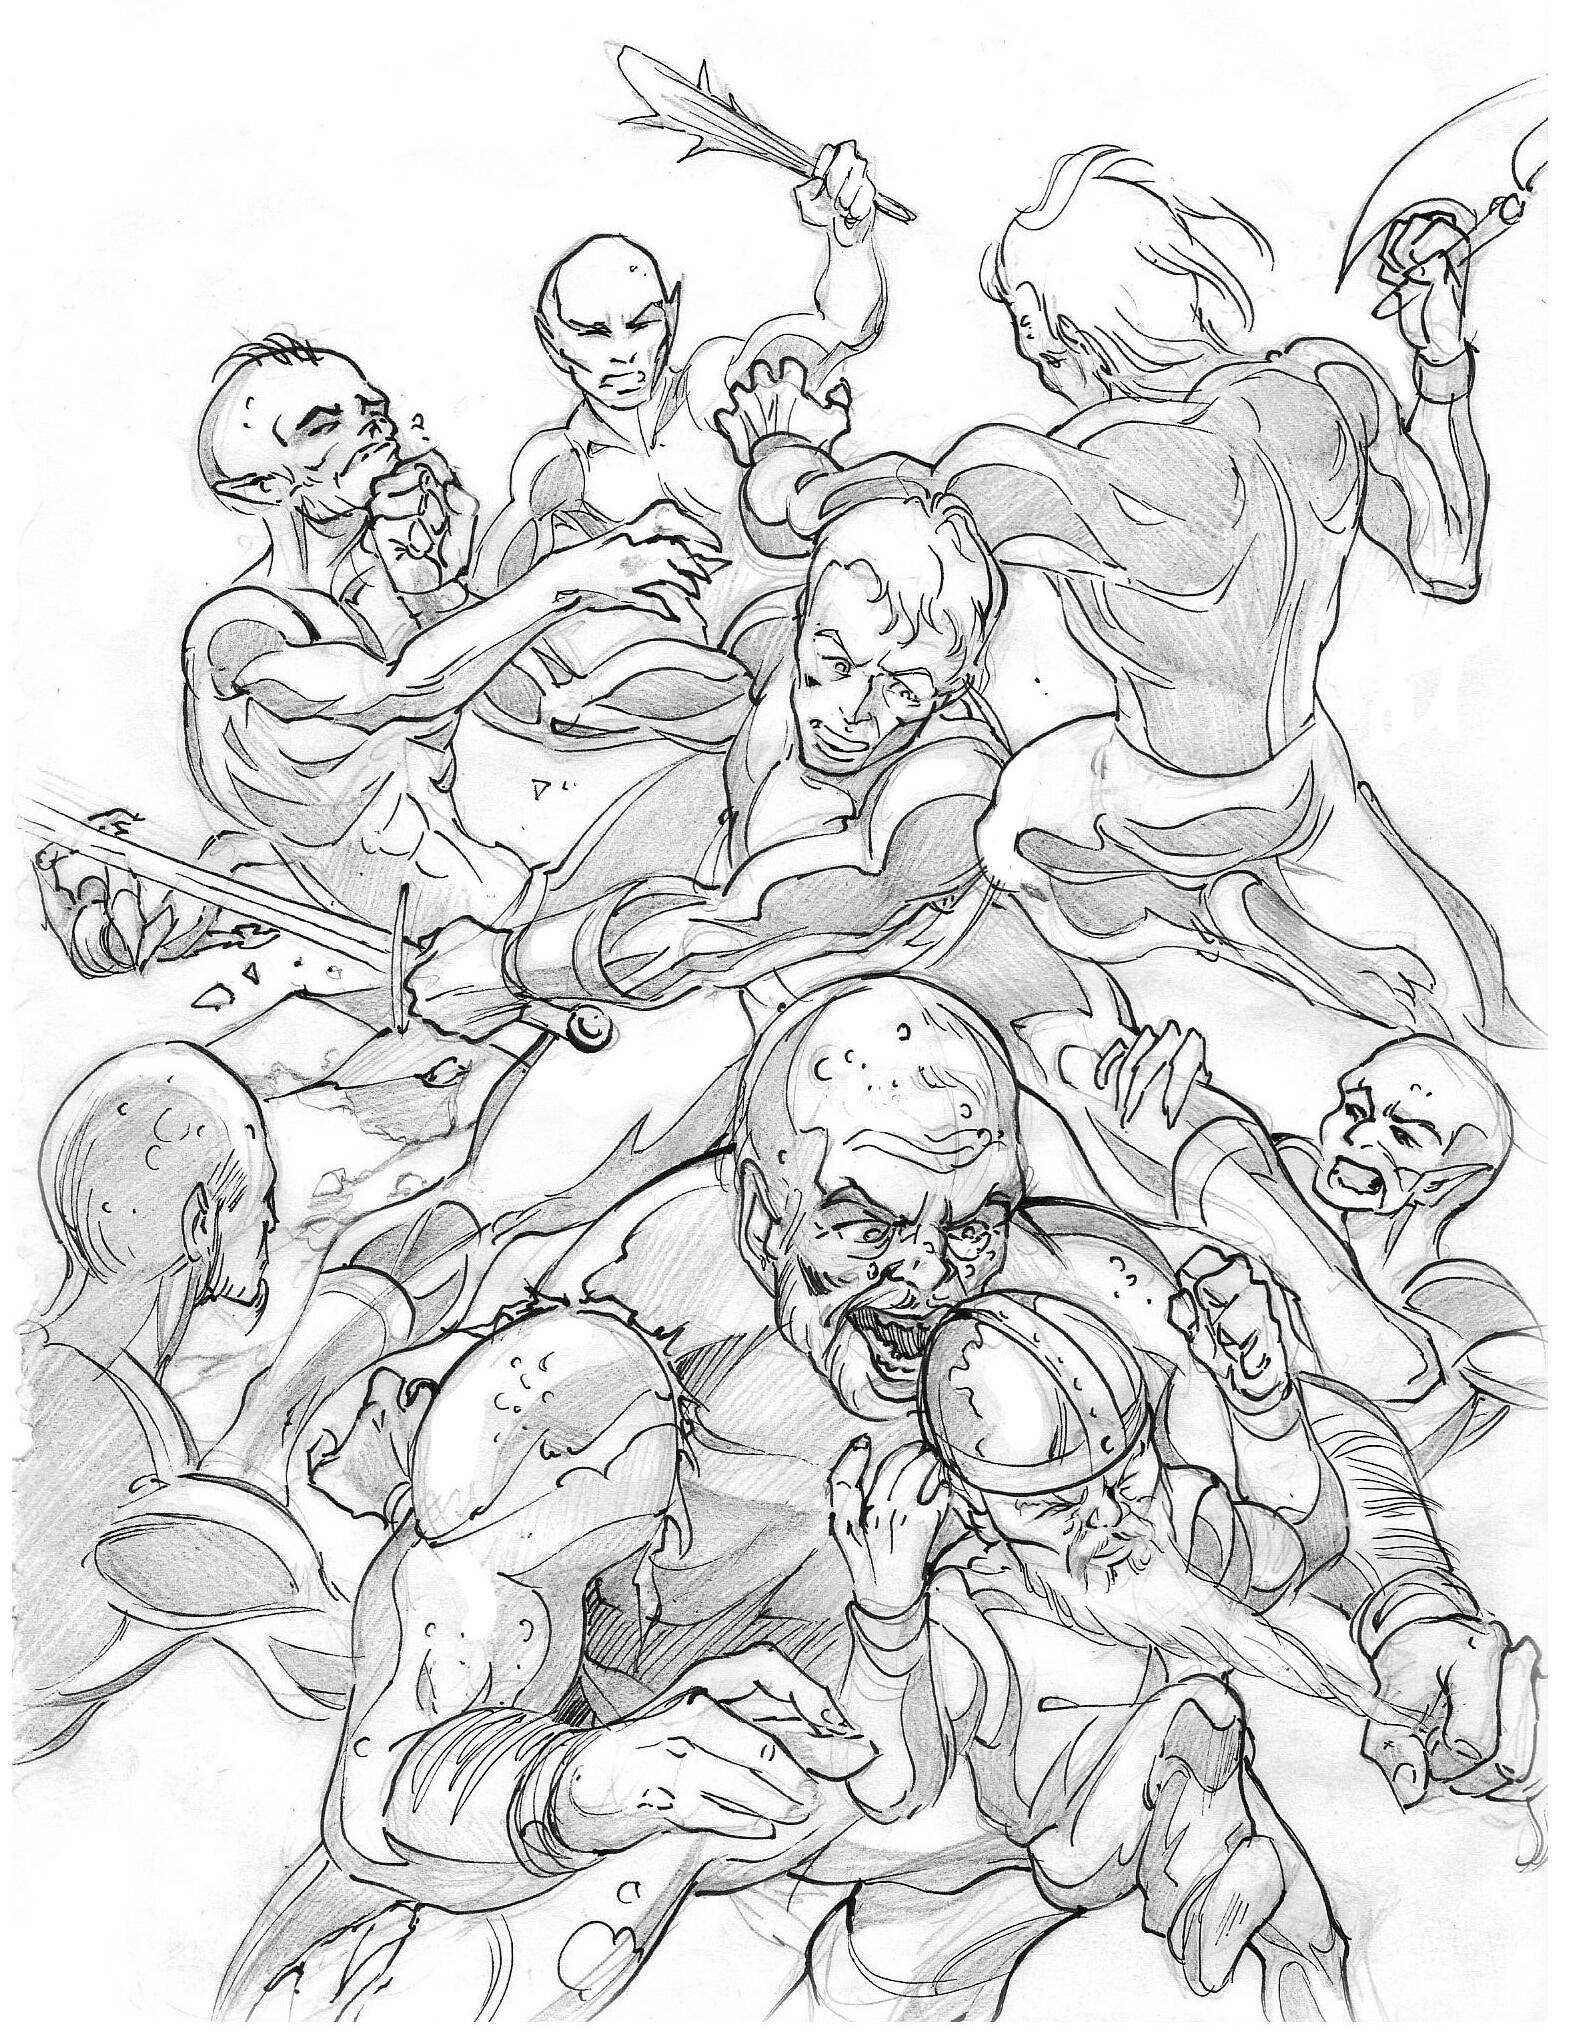
\includegraphics[width=.6\textwidth]{images/Boris_Pecikozic/nura_brawl.jpg}
	\end{wrapfigure}

	The trio climbed for a while longer, looking back every few moments to note how close the nura were behind them. An ogre was among their ranks - a human transformed into a nura. That made no sense. Thenton recalled what he had read about nura - they came out from under the ground and ate entire villages. If their hunger was sated and there were still more people they would take any prisoners underground, transform them into more nura and then go back up for another raid. While captured dwarves turned into hobgoblins, ogres were made from mutated humans. But they'd had no time to return deep underground.  How did they managed to trap and transform this man while in the village?

	Looking back, the enemy was nearing and everyone was out of breath. Arneson suggested a rest to make sure they would be ready for the fight - they could fight downhill against an enemy fatigued from walking upwards. He calmly got out the rations - some cheese, smoked pork, oatcakes and a flaggon of wine.

	``May as well have the best of the rations now, eh, friends?'', Arneson said while smiling, and they slowly masticated their age-hardened meal and tried to smile back as the nine foot monstrocity which was so recently a man made its way up to them, pounding its great feet up the mountainous slopes, surrounded by half a dozen hobgoblins, each the size of a broad-shouldered man.

	As the hobgoblins neared the plateau where the trio sat they began to make their war cries, but Arneson just sat and ate his last oatcake slowly. They began to sprint upwards across the rocky ground.

	The \gls{gm} decides that since the players have the higher ground, they will receive +1 to all rolls until the hobgoblins can reach slightly higher ground - probably after the first action. One of the players must roll Initiative, so Arneson's player take the dice and rolls, producing a `5'. Each character's Initiative Bonus adds to this separately, so Thenton's Initiative of +1 gives him a total of 6; Hugi's Initiative of +0 gives him a total of 5 and Arneson's Initiative Bonus of +2 makes his total 7. The group then gain +1 each due to the higher ground. Meanwhile, the nura have rolled a `5' for their Initiative as well. The hoboblins each have a +1 bonus to Initiative and the ogre has a +0 bonus.

	The \gls{gm} knows the highest Initiative total is somewhere under 9 so she calls out,

	``Ten! The nura gather at the base. Nine! They cover their faces with their weapons and gang together. Eight! They push forwards and ....''

	``Eight!'' shouts Arneson's player. ``I'm going at eight! \ I'm going for the ogre - you said he was unarmoured so we should be able to take him down with a couple of good hits''.


	Arneson's player needs to roll an 8 to hit the ogre, so he rolls and adds +1 for his Combat Skill. His total is `11' and he hits. He has already rolled his damage die at the same time. It landed on a `2'. He adds +2 for his Strength and +1 for the sword's Damage bonus for a total of 5. The ogre shrieks in pain as Arneson's sword sticks in. Arneson's action took 6 Initiative points so he goes down to `2', and the hobgoblin has spent 2 Initiative to defend himself.

	``Seven!'', she cries. Thenton's player jumps in. He only deals $1D6+2$ Damage but he has a much better Combat Skill of +2. He rolls to Strike but misses the ogre with a `5'. His Initiative score reduces to 1, and he reduces the hobgoblin's from 6 to 4.

	``Six!'', beckons the \gls{gm}, and starts to describe leering hobgoblins stabbing at everyone's feet from the base of the great stone step the trio are sitting on. She gives them each a -1 to attack due to occupying the lower ground.

	A hobgoblin hits Arneson, so he spends 2 Initiative to attempt to Dodge. Arneson rolls a 7 -- not enough! The hobgoblin's Strength is +2 and the battle axe adds +3 Damage for a total of +5. 4 of the Damage is replaced with a die, so the hobgoblin is rolling $2D6+1$ Damage. The total is 6. Arneson's player first reduces that by his chainmail's \gls{dr} of 4, leaving 2 Damage. Instead of taking that Damage he marks off 2 \glsentrylongpl{fp} and declares that the attack in fact misses.

		Hugi finally releases his crossbow, but in all the confusion misfires. He's down to Initiative 1.

		\needspace{3cm}
		\begin{wrapfigure}{r}{.3\textwidth}

			\begin{tabularx}{.3\textwidth}{c|X}
				\setcounter{enc}{12}

				8 & Arneson deals 5 Damage to a hobgoblin. \\

				7 & Thenton misses. \\

				6 & Most hobgoblins attack. \\

				5 & Ogre grabs Hugi, then runs away. \\
				4 & Two hobgoblins attack. \\


			\end{tabularx}

		\end{wrapfigure}

	``Four!'', shouts the \gls{gm}, then she smiles. The next hobgoblin attacks and Arneson rolls a 5 -- that's a failure with a Margin of 4, so it bypasses his chainmail. The axe is coming down towards his unarmoured shin-bone and the Damage rolled is 9. He marks off his last 9 \gls{fp} rather than taking any Damage. Any further Damage is coming straight off his \gls{hp}.

		``The ogre pushes forward with its club then reaches out to grab Hugi. Roll at \glsentrylong{tn} 9''.

		Hugi's player isn't happy, as that is enough to hit him, or in this case grab him. In fact with his crossbow out rather than a defensive weapon, he'll have a hard time defending himself.

		The ogre reached forward, grabbing Hugi by the beard and pulling him back through the horde of nura and out from the protection of his companions.

		The other players want to attack the ogre, but he's making a movement action - these count as Quick Actions so they are allowed to operate before other actions. Hugi disappears behind the crowd. The ogre's Initiative reduces to 0 and he is done for the \gls{round}, but Arneson and Thenton each have one action left.
	\end{exampletext}

}{}

\section{Complications, Options \& Manoeuvres}

\subsection{Brawling}

\index{Combat!Brawling}\index{Brawling}Punches and kicks all use the Combat bonus. Such attacks inflict Fatigue Damage. Everyone gains a \gls{dr} against Brawling Damage equal to their Strength Bonus, which stacks with armour (\gls{dr} cannot be negative). This counts as Complete armour, so hitting someone in Partial chainmail with a \gls{tn} of 8 and a Strength of +1 would mean they have a total \gls{dr} of 6. However, an attack score of 11 would mean that the Partial armour's \gls{dr} could be ignored, leaving only a \gls{dr} of 1. An attack score of 13 would ignore both types of \gls{dr}, leaving nothing at all. Attacks which bypass a body's natural armour count as normal Damage as such attacks might hit vulnerable locations such as the eyes or crotch or twist an opponent's arm till breaking point.

\subsection{Blind Rage}\label{blind}

\index{Blind Rage}Weapons can grant a bonus to the wielder's Evasion Factor because the wielder is keeping people at bay with it -- a spear might be waved in an opponent's face in a threatening manner or a sword might be on the ready to attack if someone gets within its range. However, this marvellous defence only works against people who care about being hit. Anyone can choose to attack someone while ignoring their opponent's weapon's bonus to Evasion; the penalty is simply that the opponent can choose to make a single Sneak Attack immediately. This counts as a Sneak Attack, gaining +4 to hit and +2 Damage.\footnote{See page \pageref{sneakattack}.}

\subsection{Blindness}

\index{Blindness}\index{Combat!Blindness}Fighting while blind is no fun -- your opponent can see you coming, and you can't see them. Blinded opponents suffer a penalty equal to -8 plus their Wits and Vigilance Bonuses with a maximum penalty of -6. For example, a character with With -1 would receive a -9 penalty to attack, except that the maximum penalty is -6. Someone with Wits +1 and Vigilance +3 \ would suffer a -4 penalty to attack because both reduce the basic penalty of -8.

This penalty only counts when one side of a fight is blind. When both sides are blind, we use the Darkness Fighting rules below.

While fighting blind, if the dice make a \gls{natural} roll equal to the number of people on their side (including themself) then they hit a companion. If the character is fighting with just one companion then there are two of them and they hit a companion on the roll of a 2. If they are part of a group of 5 people, any roll of 5 or under means they have accidentally hit a companion. Companions who are are accidentally hit can attempt an Evasion roll by rolling with their current Evasion Factor against \gls{tn} 10; failure implies normal Damage from that attack. It is quite possible to kill a companion while fighting blind.

\subsection{Darkness}

\label{darkness}\index{Darkness}Fighting in the darkness, or just twilight, can give a distinct advantage to those with sharper senses. Those who retain some basic vision while their opponents have none are in a similar situation to fighting a blinded opponent. However, when both sides suffer from the darkness, the battle changes very little. Neither side can hit very accurately, but then neither side can dodge or parry very well either.

When fighting in the dark, each side receives a penalty to attacking the other equal to the difference between their respective Wits + Vigilance totals, up to a maximum of -6.

For example, a human guard has caught a room full of elves with stolen goods. Thinking quickly, one of the elves douses the room's only lantern. The human has a Wits Bonus of -1 and no Vigilance Skill. The elves have a minimum Wits of +1 and many also have the Vigilance Skill; that means the elves will receive a +2 bonus to striking the guard and those with the Vigilance Skill will receive a higher bonus.

Deep darkness can provide a maximum penalty of -6, while twilight is limited to a penalty of -3.

\subsection{Drawing Weapons}

\index{Combat!Drawing Weapons}Drawing a weapon costs 2 Initiative if it is placed in an easy place to draw, like a scabbard on the side of a belt. If a character holds weapons on the back or in a bag, it costs 8 Initiative to remove them. If a knife's stuffed inside a pack, the \gls{gm} may stipulate a number of \glspl{round} required to draw the weapon.

\subsection{Flanking}

Attacks from someone's anterior side gain a +2 Bonus.  Anyone caught alone is in more danger than they would be, due to opponents attacking from all side.

\subsection{Grabbing \& Grappling}\index{Combat!Grappling}

\subsection{Grabs}

A grapple always starts with a grab.  A grab is a normal roll, made without any benefits from weapons.  If successful, the character has grabbed an opponent.

Once two people are grappling, neither can move and so both can be struck as per a Sneak Attack by anyone nearby.

\subsection{Grappling}

Once two people are caught in the grapple, either can make a grappling roll at the cost of 4 Initiative.  They can then roll with double their Strength, plus their Strike factor, against 7 plus the enemy's Evasion score.

A successful roll implies the character can break the grapple and move freely, or can inflict $1D6$ plus their Strength Bonus in Damage.

\subsection{Guarding}\index{Guarding}

If you guard someone by standing in front of them then all attacks have to go through you first.\footnote{This includes missile attacks only if you could otherwise evade them.}  Any enemy making a successful attack on you can choose to damage you, or to make another roll (as a free action, costing no Initiative) at their real target.

\subsection{Half Swording}\index{Combat!Half Swording}

It is possible to hold a sword by the blade and use the guard to bludgeon one's opponent. This manoeuvre allows the weapon's Speed Bonus to be added to its Damage instead. It takes 2 Initiative points to change how one holds the sword.

\subsection{Holding Off}\index{Combat!Holding Off}

Anyone can wait to see what the battle brings -- the character simply lowers their Initiative and can jump in at any point, acting at one Initiative higher than a declared action.

For example, someone might hold off their action at Initiative 5. They wait for the enemy to attack at Initiative 3 and notices that one of them is attempting to use a magical item. Immediately they retroactively performs an action at Initiative 4.

\subsection{Keeping Edgy}\label{edgy}\index{Keeping Edgy}

The character can take a moment to note their \index{Dodge!Long-range}long-range surroundings, including archers and potential spell casters. This takes only 2 Initiative points and for the rest of the \gls{round}, any time the character is being fired upon in combat they can use their basic Speed Bonus in a resisted action to leap out of the way of an incoming missile or targeted spell, such as a fireball. Spells which simply target people by gaze or magical effects such as polymorphing are unaffected.

\subsection{Passing Attacks}\index{Combat!Passing Attacks}

When someone is attempting to run past others, they have some opportunity to hit when the character is passing. This can be any normal attack, but counts as a Quick Action, jumping ahead in the Initiative Score. The attack costs the normal amount of Initiative.

\subsection{Ram}\index{Combat!Ram}

In combat, it is possible to scare, push and stab at someone to force them to move backwards. The attacker spends 3 Initiative points. The defender can either attempt to resist, or can simply acquiesce and move back. When moving back, targets are pushed back 2 square; the attacker's Strength adds to this and the opponent's Strength decreases it. Characters can sacrifice the use of 1 point of Strength to push back an additional person.

Those who resist must also sacrifice 3 Initiative. A resisted Strength + Combat Skill check is made. Successful resistance means that the defender is not pushed back.

A \textit{Ram} action must employ normal movement, and cannot move any character farther than their normal movement.  Characters who have been rammed but are unable to move far enough back fall \textit{prone}.\footnote{See page \pageref{prone} for details on falling prone.}

\subsection{Sneak Attacks}\label{sneakattack}\index{Combat!Sneak Attack}

When taking someone by surprise, the attacker gains a +4 bonus to the attack and a +2 bonus to Damage. Opponents cannot use any Evasion bonuses from Dexterity, weapon Bonuses or the Combat Skill.

Sneak Attacks also gain a penalty equal to the weapon's Weight Rating (if positive).  Warhammers are not the best choice for assassination weapons, while daggers and handaxes do much better.

Sneak Attacks can happen mid-combat when someone is ignoring a flanker's attacks, when creeping up on someone from behind, or simply when planning a daring attack.  The attacker might use Dexterity + Stealth to sneak unseen, or Intelligence + Stealth to pick the perfect ambush spot.  Defenders usually use the same Attribute + Vigilance.

\subsection[Spell Casting in Combat]{Spell Casting in Combat}\index{Combat!Spell Casting}

Spell casters are assumed to be focussing on their spells and using both hands for that purpose rather than weapons. They use their Wits for the Initiative bonus rather than Speed and receive no Combat Skill Bonus to Evasion -- they only use their basic Dexterity score.

Casting one-handed is possible, but difficult. Any roll the spell requires receives a -2 penalty. If the spell requires no roll then it is assumed it requires no hand movements and therefore gains no penalty. Casting one-handed allows the caster to hold a weapon in the other hand, for either defensive or offensive purposes.

Spell casters who wish to both attack and cast spells within the same \gls{round} must use the lower of their Speed and Wits score when determining Initiative. They can then use their full Combat Skill Bonus for the \gls{round} to add to the Combat Factors but cannot take their Initiative Factor higher than their Wits Bonus.

Switching away from one's focus on spells or martial combat must be decided at the start of the \gls{round} -- mages who are not mentally prepared to cast spells or use a sword cannot do so at a second's notice.

\subsection{Two Weapon Combat}\index{Combat!Two Weapons}

A character using two weapons -- perhaps a shield in one hand and a sword in the other -- can use the best Speed, Strength and Dexterity bonus from all weapons. Each weapon will have to be held in one hand, increasing its Weight Rating by 2.

Shields, uniquely, can add their Evasion Bonus to the character's Evasion Factor even while the wielder is in the Aggressive Stance. As a result, someone could use a shield's bonus to Evasion while using a sword's Evasion Bonus to add to their Strike Strike score. In this case, Dexterity would always be added to Strike, along with the sword's Bonus.

\section{Combat Summary}\index{Combat Summary}

\begin{enumerate}
	\item Characters publicly declare stances. If no stance is declared, assume a Defensive stance. The \gls{gm} rolls for enemy Morale if appropriate.
	\item Each character divides the Combat score (if any) between Initiative, Strike and Evasion.
	\item The leader of each group rolls Initiative and each character adds their own Initiative Factor.
	\item Actions are resolved in order of Initiative, each reducing the Initiative score.
\end{enumerate}

\iftoggle{verbose}{

\begin{exampletext}
	Arneson decides he is going to push through the crowd to save his friend. Pushing the half dozen nura back is going to be tricky. He launches himself from the stony step they are on, pushes his chest into one then grabs two more hobgoblins. Since he is pushing back 2 extra figures, he takes a -2 penalty to the action. Arneson's rolling with +2 from his Strength Bonus and +1 bonus for his Combat Skill for a grand total of +1. The \gls{tn} is 7 plus the hobgoblins' Strength of +2 and Combat Skill of +2 for a total of 11. The \gls{gm} allows him a total of a +2 bonus for jumping off the step. The dice come up with an 8 and his total of +3 just passes the test. Normally, he would only push the nura back by 1 step, but they are on the side of a cliff and being pushed onto their back feet.

	The \gls{gm} decides some sort of check is in order to see how well the Nura perform. Ordinarily, she would roll for each of them but there are six of them and that will take too long. Thinking quickly - because who wants to slow down combat? - she decides that all of them could potentially fall down the cliff since the first three are in front of the next three so Arneson is pushing against all of them one way or another. She gives them a \gls{tn} of 9 to stay up and a bonus of +6 because there are 6 of them. Each Margin they roll in the final score is one hobgoblin that has not fallen over. Dice clatter, she has rolled a `4' and that leaves a final score of 10. Everyone falls down the mountain's steep incline except for a single nura.

Thenton, on Initiative 1, is the last to act. He jumps off the cliff-side to attack the last hobgoblin. He strikes with a score of 11, bypassing the ugly creature's Partial chain armour, then rolls $1D6+2$ for the Damage for a total of 4. The creature is reduced to half its hitpoints with a crimson gash across its throat.

As Thenton's sword swooped down it opened up his target's arm. The last one standing cries out and withdraws his arm then backs off.

	``End of the \gls{round}!'', cries the \gls{gm}. ``Round two! Roll for Initiative''.
\end{exampletext}
}{}

\section{Ranged Combat}
\index{Ranged Combat}Projectiles have their own Skill which is bought just like the Combat Skill and always add the Dexterity Bonus to make an attack. Archers roll to hit and then Damage, just as with Combat. The \gls{tn} is always 6 plus one for every five full squares away the target is. Targets 14 squares away would have a \gls{tn} of 8 to hit. Most targets cannot use any weapons to add to their Evasion Factor (except shields) but can use the Speed Bonus to evade missile attacks if they are on the run or Keeping Edgy.

Just as with weapon combat, a high enough roll can be a Vitals Shot, ignoring all \gls{dr}.

When someone with a bow is attacked, they can use their Combat Skill and Dexterity to Evade as per usual.

\subsection[The Long Bow]{The Long Bow}
\index{Long Bow}\index{Bows}Long bows (or `hunting bows') are difficult things to work but well worth it once the archer practices enough. To pull back the heavy load on a long bow takes 2 \glspl{round}, and the arrow flies at the very end of the second turn. Each bow has its own Strength rating and anyone without at least that much Strength cannot use the bow; the bows deal $1D6$ +Strength Rating +1 Damage. So if a bow has a Strength rating of 2 then it deals $1D6+3$ Damage but requires a Strength of 2, at least, to operate. Having a Strength of 3 will not increase the Damage.

Long bows can be fired for hundreds of yards -- the maximum range is generally more determined by the archer's ability to aim than by the range of the bow.

\subsection{The Short Bow}
\index{Bow!Short Bow}\index{Short Bow}A short bow, or `trick bow', is a smaller, lighter thing which can be used by anyone. What it lacks in punch it makes up for in quick draw time. As usual, for every two squares beyond the first two the archer suffers a -1 penalty to hit. The bow takes 4 Initiative points to fire so many shots can be fired in a \gls{round}.

Short bows have a maximum range of 20 squares and deal $1D6-1$ Damage. They often bring down prey by multiple arrows rather than the one.

Firing a short bow requires 4 Initiative points but reloading takes another 2.

\subsection[The Crossbow]{The Crossbow}
\index{Crossbow}Crossbows can be powerful, but are not easy to reload. They have a basic Damage of $1D6+2$ though different crossbows vary in quality. Crossbows take a number of \glspl{round} to reload equal to 5 minus the character's Strength score. Firing a crossbow takes only 3 Initiative points.

\subsection[Thrown Weapons]{Thrown Weapons}
\index{Thrown Weapons}Thrown weapons such as knives, spears or others are typically not great at killing enemies, but they can certainly wound them. They work just as shortbows, but their Damage is the normal weapon Damage -2. Someone with Strength +1 throwing a dagger would deal $1D6$ Damage, while someone with Strength -1 would deal $1D6-2$ Damage.

Weapons which were never made to be thrown, such as swords or axes, receive a -2 penalty to hit, i.e. they are thrown at a basic \gls{tn} of 8 rather than the usual 6 for projectiles.

\iftoggle{verbose}{

	\begin{exampletext}

		``Remember your attack stances this time everyone'', says the \gls{gm}.

		\begin{wrapfigure}{r}{.3\textwidth}

			\begin{tabularx}{.3\textwidth}{c|X}
				\setcounter{enc}{12}

				10 & Ogre grapples Hugi. \\

				7 & Thenton moves to stab the Ogre. \\

				6 & Ogre deals 5 Damage. \\

				5 & Thenton kills the ogre. \\


			\end{tabularx}

		\end{wrapfigure}

		The players wonder if they want to add their Dexterity Bonus and Weapon's Evasion Bonus to Strike opponents instead of Evading attacks, but at this stage defence is more important, especially for Hugi - currently being pinned down by an ogre, and Arneson, currently down to only his Hit Points.

		Next up, players assign their Combat Skill. On the last \gls{round}, they left it as the default - it added to the Strike Factor. Arneson repeats the move and Hugi has no Combat score to speak of, but Thenton has Combat +2. He knows speed is of the essence if he wants to save his friend, so he adds +2 to his Initiative Factor, giving him a total of +3.

		The characters roll to get their bearings but achieve only a `4', so Thenton will act at Initiative 7. The \gls{gm} rolls for the nura and achieves `9' - with Speed +1 they will act on Initiative 10.

		``Twelve!'', the \gls{gm} rolls a Morale Check for that last hobgoblin. It is wounded and outnumbered. The \gls{tn} is 12 and it can add its Combat bonus, but the roll still fails.

		``The last hobgoblin backs up. \textit{Eleven!} It flees down the mountain towards its allies, many of whom are still rolling down the hill.''

		``Ten!'', the \gls{gm} continues, and immediately rolls for the ogre as it tries to eat Hugi's face off. This will count as a grappling roll, so he and Hugi will use double their Strength Bonus added to their Combat Skill. Unfortunately Hugi has neither Strength Bonus nor Combat Skill, so the ogre gets a straight +12 bonus; the roll succeeds before it is even made, and succeeds by a margin of 3: that means Damage is inflicted. The ogre only adds Strength - of course his massive club is useless for the attack. His Strength of +5 means he will roll $2D6+1$ Damage for a total of 4. Hugi is safe for now as the ogre luckily bites down on dwarvish helmet as Hugi's player marks off 4 FP.

		``Nine! The ogre pulls Hugi down. Eight! He bites down on Hugi's face but gets a mouthful of helmet instead. Seven!''
		Thenton's player is acting now and takes two Initiative to run over to aid Hugi. He asks the \gls{gm} if he can sneak up on the ogre.

		``You mean in the middle of a fight you want to backstab someone?''

		``Sure. He's busy eating Hugi's face, so can I stab him while he's not bothering to avoid it?''

		The \gls{gm} thinks about it - the action is not clearly covered in the rules, so she decides the following.

		``Okay - make a sneak roll. If he sees you then he's going to stop the action and defend himself, otherwise your next attack can count as a Sneak Attack. Roll Speed + Stealth at Target Number 6.''

		Thenton has no bonus to either, but that ogre is so dim the test is easily passed. 

		``Six! The ogre gnaws into Hugi's face, this time without failure. 5 Damage!''

		Hugi's player marks off his last 3 FP then 2 HP, noting that he could have just died if the dice had rolled higher.

		Arneson runs over to aid the fight.

``Five! Thenton rolls for attack''

His Sneak Attack gives him +4 to strike the ogre - which he does - and +2 Damage, making his Damage roll $2D6$. His total is 7 Damage.

		``Launching himself forward he lands the tip of his sword into the ogre's back just as teeth are sinking into the dwarf's face. It finds purchase and slides in only six inches before stopping. The giant whirls \gls{round}, ripping the sword out and pushing Thenton to the side. He screams and attempts to get up, then slumps back down onto the dwarf, blood pooling out of the gash on his back''

``Finally!'', shouts Thenton. We're done. It's finished. We can {\dots}

``Four! Over a dozen hobgoblins can be seen marching down from the mountain.''

``What? \ We can't handle any more. Hugi's Damaged. Arneson's in poor shape too.''

``Three! \ They pull out crossbows and start cranking them {\dots}''
	\end{exampletext}}{}

\section{Morale}
\newcommand{\moralechart}{
	\begin{tcolorbox}[title={Moral Chart},arc=1mm,tabularx={cp{.75\textwidth}}]
		\gls{tn} & Situation \\\hline

		-4 & Monsters outnumber characters 3:1. \\

		-2 & Monsters outnumber characters 2:1. \\

		+2 & Characters outnumber the monsters. \\

		+2 & Monster is wounded. \\

		-2 & Characters' top Strength Bonus is 2 lower than the monster's highest Strength Bonus. \\

		+2 & Character's top Strength Bonus is 2 higher than the monster's highest Strength Bonus. \\
	\end{tcolorbox}
}

\moralechart

\index{Morale}Most combats will end with one side or the other running away -- few troops want to fight to the last man when they could potentially be safe at home by the end of the day. At the start of each \gls{round}, the \gls{gm} rolls a morale check for the enemy if they think the enemy have a good reason to flee.

The players do not take morale checks -- they decide when it's time to run away by the look of the situation. Usually a good time is when all the \gls{fp} have run out.

Moral checks are rolled at \gls{tn} 6 with a character's Combat Skill (or Aggression Skill if the character is an animal). As usual, the \gls{gm} rolls for an entire group with one roll. If the characters have just attacked a group of 10 hobgoblins and injured 3 then the troop will roll at \gls{tn} 6 to see if they should flee, but the injured 3 hobgoblins roll at \gls{tn} 8. If the final result is a 7 then all of the hobgoblins will remain except for the three injured ones.

When an enemy flees the scene, characters gain half \gls{xp} if they had engaged them in combat.

\iftoggle{verbose}{

	\begin{exampletext}
		Thenton's mind was racing - searching for anything to help he remembered his acting classes, the roar they taught to open a grand scene and how actors said their roar was such that it would terrify local ruffians around the town.

		Thenton's player asks the \gls{gm} about making a moral check for the hobgoblins.

		``Well'', she ponders, ``you certainly don't outnumber them. They are not half dead. They might make a moral check at \gls{tn} 4 but they would get a +1 bonus for their Combat Skill. So no, not really. They are not terrified of Thenton waving his sword about, even if he took acting classes''.

So much for that plan.
	\end{exampletext}
}{}

\section{Chases}
\index{Chases}Chases form some of the most dramatic scenes in an adventure. When running on an open field without any barriers, everyone simply runs at full speed -- whoever has the highest Speed + Athletics total succeeds in running away or catching up with an opponent. In all other situation, where there are some obstacles, alleys and such, characters can pursue, gain and lose ground and try dirty tricks.

The system is simple -- one player rolls $2D6$ for the group. Each person then modifies this group score. Since the party will probably run at different paces, they have the option of abandoning slower members or slowing down to the pace of the slowest member.

The \gls{tn} is 6 plus the enemy's Speed + Athletics Bonuses. Failure means the characters are instantly caught, before they are able to run anywhere. If the players hit the \gls{tn} they manage to run through 1 area while being chased. For every Marginal point, they run through an additional area. If the Margin is ever 3 or more then they completely evade the enemy. If the party obtain less than total success, they and their pursuers both move and must roll again.

The table is a guide to an unaltered roll. In most situations enemy Traits will affect the actual results of such a total by increasing or decreasing the \gls{tn}.

	\begin{tcolorbox}[arc=1mm,tabularx={lp{.85\textwidth}}]

	Total & Result \\\hline

	11+ & The characters immediately escape their pursuers. \\

	10 & The characters escape their pursuers after travelling through two areas. \\

	9 & The characters escape their pursuers after travelling through three areas. \\

	8 & The characters are chased through 3 areas and reroll. \\

	7 & The characters are chased through 2 areas and reroll. \\

	6 & The characters are chased through 1 area and reroll. \\

	{\textless}5 & The characters are immediately caught. \\

\end{tcolorbox}

The \gls{gm} is encouraged to give a fast-paced description of fast-moving scenery, hurriedly telling the players about a new area before moving instantly on. Each area covered holds new opportunities for getting away, or trapping the quarry -- whether that is the players or their prey.

Characters running through forests might encounter a marshy area, a stream, dense thickets, an open plain and then a sudden, steep hill. Those crossing plains might find a random encounter in their path, then a copse of trees. Those running up a mountain could find an area of loose rocks where the ground slides away from under their feet, a narrowing path upwards as rocky walls envelop them and then a misty lake covered in low-lying cloud.

Each area covered also inflicts 1 Fatigue Point in addition to any for wearing armour or for Encumbrance Points. These Fatigue Points are applied after every roll rather than waiting until the end of the scene.

Players are encouraged to suggest Skills which might help. While running away from a band of guards, a character could use the Stealth Skill, quickly dipping into an alleyway to hide. When jumping around a busy area of town, the character might leap over a moving cart to gain some headway. Characters can, with \gls{gm} permission, use their Skills to aid an entire group. The Stealth Skill, in particular, might be used to aid the entire party to hide by finding the right spot. The Empathy Skill might be used to quickly convince farmers to hide the characters.

\iftoggle{verbose}{

\begin{exampletext}
	Thenton's next plan was to run away as fast as possible. This was much more popular than his last plan, though Hugi was still not happy as he had an arrow that he had not yet removed from his shoulder. The hobgoblins of course realised that they had no time to reload so they just gave chase. They dropped their projectiles, pulled out their shortswords and started to clamber along the rocky face of the mountain. The trio could not move clearly up the mountain until they had gained some ground between themselves and the hobgoblins, and feared that there would be more openings to once-dwarven tunnels, now infested with nura, if they went further up from their present location.

	The basic \gls{tn} for such actions is 6 and the \gls{gm} lowers it by 2 because the trio have a good headstart. The hobgoblins add their Speed Bonus of +1 for a final \gls{tn} of 5. The party roll an 8 but unfortunately Hugi isn't the fastest of people - he's only four feet tall after all - so his score is 7. They needed that 8 to completely get away. Arneson and Thenton decide they're going to keep pace with him rather than running ahead. They're not caught yet, but run through three different distinct areas before making another roll.

The hobgoblins were fast on their trail as they clambered over the rocky mountain side. They soon headed up steeper, overhanging rocks and at one point had to help each other upwards across large rocks jutting out of the side as the nura horde came ever closer. Finally, they reached the peaks and gazed down the other side. Seeing only mist in the other side they decided to lose themselves in the crevices there before the enemy could catch up enough to see their direction.

	Arneson's player wants to roll again while adding his +2 Stealth Skill. He is the only one with this Skill but the \gls{gm} says he can use it to help everyone hide. The group don't get the previous +2 bonus for their head start because they are already running so the final \gls{tn} is the same. Arneson's player takes the dice and rolls; he scores 11.

	They didn't go far, but only hopped down a few stony crevices before Arneson beckoned them to the side and requested they creep into a nook he had found. Hugi and Thenton could only just fit, with no spare room, so Arneson then bounded off to see what else he could find. He was still out looking for a spot when the great axes scraping down the cliff could be heard, and guttural voices complained about dangerously empty stomachs. Deep in the misty cloud, Arneson said a silent prayer to Laiqu\"{e} that it would not be too long before the nura starved to the point of eating each other.
\end{exampletext}
}{}

\section{Further Dangers}
\subsection[Falling Damage]{Falling Damage}
\index{Falling}Characters who fall from a height suffer 2 Damage per square the character fell. 2 Damage alone converts to $1D6-2$ Damage, while 4 Damage would simply be $1D6$ and so on. Characters falling straight downward can attempt to mitigate 4 Damage by rolling Dexterity + Athletics at \gls{tn} 9. Those falling forward and down in an arc can try to roll along the ground to mitigate the Damage; they roll Dexterity + Athletics at \gls{tn} 7 and a successful roll indicates that they reduce incoming Damage by 4.

The maximum Damage someone can suffer from a fall is 18, equating to $4D6+2$.

\subsection[Marching]{Marching}
\index{Marching}Every two miles walked inflicts a Fatigue Point at the end of the day. Additional Fatigue Points for carrying heavy items and wearing armour are added as usual. Humans have an uncanny ability to walk all day without tiring, and only endure 1 Fatigue Point every 4 miles.

\subsection{Trapped or Entangled}
Characters caught in mud, who lip over, or get shackled to a spot cannot move or dodge nearly as well as they could.  They receive no benefits from their Dexterity Bonus or the Knack: Fox Hop.

\subsection{Falling Prone}\index{Prone}\label{prone}

Characters who fall over lose their ability to defend themselves, as above.  However, they can get up at the cost of 2 Initiative by using up their movement action.  If they've already moved this \gls{round}, they have to wait until the next \gls{round}.

\iftoggle{verbose}{

	\begin{exampletext}
		``That's the end of the scene'', the \gls{gm} says. ``You can each regain 2 Fate Points''

``I've got 10 Fate Points in total'', mentions Arneson's player, ``So I'm getting 4. But doesn't this rest period count as a new scene too?''.

		``Sure, says the \gls{gm}. ``Mark down another load for hiding in the tops of the mountains''

With their FP now replenishing quickly, the group can rest and worry less about being hit again.

		``Oh! I've been forgetting about the Fatigue'', says the \gls{gm}. Your \gls{gm} will probably say the same at some point.

		``Everyone got two Fatigue from being in two \glspl{round} of combat and another for doing that in armour, so mark down three Fatigue points in your Combat boxes. Then four more for running through three areas in armour. That's seven in total''.

Thenton's player has the Combat Skill at +2, so he marks those Fatigue points in the first and second boxes, leaving him absolutely fine. Then he adds another for wearing armour during that fight; since there are not more Combat Skill Fatigue Boxes, that point goes into his normal Fatigue boxes. Then he receives three more for running across the mountain and another for doing that all in armour. Five Fatigue Boxes are marked down in total. If the characters had continued being active that would be the end, but since they have finished the scene while resting, Thenton heals 4 Fatigue points leaving him with only 7 in total.

		Hugi isn't doing so well. He only had 2 HP left by the time he was running. He has no Combat Skill so he gains the full 7 Fatigue Points. Finally, the \gls{gm} reminds him that he is bleeding from his wounds. He is in no condition to patch them up while hiding, especially since nobody in the party knows anything about Medicine. She decides to only award one more Fatigue point since the arrow is also stopping the wound from bleeding too much - that makes the total 8. Hugi's rest allows him to regenerate 3 Fatigue Points (he's not as strong as Thenton) so he receives 5 Fatigue Points in total. Dwarves, luckily, can withstand 2 additional Fatigue Points so 2 of those points give him no penalty. That's 6 more than his HP. He gains a -4 penalty to all actions.

The danger now passed, the warriors lie in their hiding nooks, watching the cold clouds whirl around them, hoping to never see nura again. They breathe in and out gently, waiting for the heaviness in the chest to subside. Despite the winds, Thenton can hear a gentle drip, drip, drip from the slowly bleeding wound on Hugi's shoulder where an arrow still lies.
	\end{exampletext}
}{}

\chapter{Magic}
There are many ways to cast spells. Each magic user walks a different \glspl{path} of magic, and some walk two at the same time. Each one uses a central pool of mystical energy called mana. Characters have a certain number of \gls{mp} which they use to cast spells. Alchemists use an inner store of energy which drains them. Bards who learn to cast spells through their songs often think of themselves as having some inner store of creative energy. Priests often think of their connection to the divine as a limited pool of favour-asking which can deplete over time.

Spells are divided into different `spheres'. There is the sphere of illusion, which deals with making things appear to come into existence, then the sphere of conjuration which summons things from far away or teleports mages across great distances. Each sphere has five levels of understanding; casters must understand the first level before continuing to the second, and so on.

Each \gls{path} of magic grants access to different spheres. Illusions, for example, might be cast just as easily by an alchemist as by someone using song magic. They could not, however, be cast by someone using the \gls{path} of runes.

Each level of a sphere typically grants access to a few spells. Those learning to cast magic don't think of spheres as having discrete levels'; they think in terms of a dozen different spells for each level, but for simplicity's sake we record groups of spells together. While an alchemist will first learn to enflame a candle, to snuff out a lantern, then learn another spell to zap enemies from afar, and a different one for nearby enemies, we will call the entire thing `Invocation 1'.

\subsubsection{The Spheres of Magic}
\paragraph{Aldaron} allows one to enchant animals then later to harness control of the local weather conditions.

\paragraph{Conjuration} changes things from one form to another, and eventually can summon items out of the air.

\paragraph{Enchantment} allows casters to heal and calm people's mind, and soon after the enchanter learns how to twist people's mind to confusion others to the point of inaction.

\paragraph{Fate} is divine magic and allows the caster to ask a question of the gods, then later to heal companions' Fate Points.

\paragraph{Force} magic is a very versatile sphere, allowing the mage to protect hirself, fight with levitating weapons or just levitate any object or person.

\paragraph{Illusion} allows the caster to summon apparitions of anything. The caster might hide a door by making an illusion of a wall over it, or create the image of a sleeping bear to frighten people. More skilled illusionists can disguise themselves as other people or creatures.

\paragraph{Invocation} is the magic of fire, lightning and destruction. It begins with bolts of lightning and later allows the caster to incinerate large swathes of enemies with great balls of fire.

\paragraph{Metamagic} is a sphere which enhances all other magical spheres, allowing spells to be cast at long range, then enhancing the mage's mana storage and letting hir counter other magical spells.

\paragraph{Necromancy} first deals with making the caster close to death so sie can feel no pain and interact safely with the risen dead. Later the necromancer learns to summon simple spirits into the bodies of the dead to make them rise as an army.

\paragraph{Polymorph} allows the caster to transform into other races, and then into entirely different species. Exactly which type of animal a caster can transform into depends upon hir body type. Lithe characters will find it easier to turn into a bird, while stronger people will find stronger animals, such as bears or warthogs, easier.

\section{Casting Your First Spell}

\subsection{Casting}
Spells are cast by spending a number of \gls{mp} equal to the spell's level, so 1st level spells always cost 1 \gls{mp} and 3rd level spells always cost 3 \gls{mp}.  The character then makes a roll against some \gls{tn}, and if the roll succeeds, the mage spends the mana and casts the spell.

\index{Mana}\subsection{Mana}

Mana is a fickle thing -- when lazing \ around a village it can take hours to regain even a little driblet of magic. When fighting in deep caves, a few minutes' focus can summon most of a mage's magical energies back. Every scene, characters regenerate 2 Mana plus their Wits Bonus. If this total would be 0 then the amount of time required to gather a single \gls{mp} increases by 1 scene. Characters with a Wits score of -2 must wait 2 scenes before regenerating 1 \gls{mp} while those with Wits -3 must wait 3 scenes.

Anyone can buy some base \gls{mp} which is then modified by their Intelligence.\footnote{See the section on Experience, page \pageref{xp}, for costs of base \gls{mp}.} For example, someone with Intelligence +1 who buys Base \gls{mp} 2 would have a store of 3 \gls{mp} to cast spells. Those with a Base \gls{mp} of 0 can still have some \gls{mp} if their Intelligence Bonus is positive.

If a caster has no \gls{mp} left, they can still cast spells by paying the cost with HP instead of \gls{mp}. The magical energies pull the power they need from the blood and bones of the caster, leaving them with a bleeding nose, raging headache and sometimes stranger effects such as acidic pustules or discoloured skin patches. Many a desperate caster has died through the use of their own magic rather than an enemy's sword; a wizard with their back to the wall is a dangerous opponent indeed.\iftoggle{verbose}{\footnote{\Glsentrylongpl{hp} cannot be spent instead.}}{}

\subsection{Range}

Unless otherwise stated, spells have a range equal to five squares plus the character's Wits score. Magic extends all around the character but mages can rarely affect targets anywhere near the range of a good archer.

\subsection{Duration}

Some spells are instant -- a ball of fire flashes from the mage and incinerates someone, or a touch grants the favour of the gods, healing FP -- but most are continuous. Continuous spells can be cancelled at will or maintained indefinitely. However, while they are being maintained, the \gls{mp} required to cast them remains spent, lowering the mage's maximum \gls{mp}.

For example, Tauron the elven sorcerer casts a spell on himself to appear as a gnome -- all the better to blend into surrounding society. He spends 1 \gls{mp}. Later, he enchants an animal to be his companion for 2 \gls{mp}. Normally, his maximum \gls{mp} is 6, but he is currently reduced to a maximum of 3 \gls{mp} so long as he continues to be a bear-riding gnome.

These still-active spells are known as \glspl{standingspell}. Some mages operate by continuously casting different spells and then going `empty' when the mana is gone. Others typically operate with \gls{standingspell} alone, casting everything they might need before the day begins and leaving their useful spells `running' but leaving themselves unable to cast more.

\subsection{Spell Types}

Your standard spell takes a while to cast -- normally 1 \gls{round} per level, so a Level 3 spell would normally take 3 \glspl{round} to complete.  Casters can go slower or faster and gain bonuses or penalties to their roll.

\subsubsection{Ritual Spells}

Mages who take their time over spells can attempt a Ritual Spell -- they cast it as a Resting Action.\footnote{See page \pageref{restingactions}.} The mage can gain mana slowly, spending some, drawing more from a mana stone or item, then spending more before finally casting the spell. The mage can gather a number of \gls{mp} equal to double their normal maximum \gls{mp}, ignoring \glspl{standingspell}. Ritual spells can also be cast as a team effort -- any number of spell casters who are on the same \gls{path} of magic can cast any spell they all know together. They can each invest \gls{mp} to create \gls{standingspell}, and thereafter any one of them can cancel the spell.

\subsubsection{Subtle Spells}

Casting an illusion or enchantment on someone with a flashing, loud and generally obvious spell can be quite a give away. Any caster can attempt to cast a spell while simply whispering and moving their hands slowly and subtly.  The \gls{tn} is raised by +2 as this is a very difficult way to cast anything.

People around the mage can still sometimes spot a spell being cast. They use their Wits + Academics in a resisted roll against the mage's Dexterity + Deceit.

\subsubsection{Quick Spells}

Quick spells can be completed in a \gls{round} or faster, costing 3 Initiative points plus the level of the spell. Such spells always force a little `flash and bang' out as the raw magic hits the air. Some mages create sparks as they cast spells, others summon dark mists -- it all depends upon the Path of Magic the mage is walking.

Quick Spells are challenging, and require the mage know a spell intimately.  They cannot be cast with the mage's highest spell level.  A mage with Polymorph at level 3 cannot cast level 3 as a Quick Spell.

\subsection{Spell Enhancements}

Some spells can be enhanced by adding additional levels.  First level conjuration spells can be enhanced by making them `Enlarged', at +1 level, or can target `Basic Metals' at +1 level.  This means the caster can cast a standard 1st level transformation spell at level 2 in order to make it `enlarged', and cover a wider area.  Enhancements can even be combined, so a conjuration spell could target a large amount of metal by making it `enlarged', and adding another enhancement to affect basic metals, such as copper.

\enhancement{2}{Example Enhancement}

This is a spell enhancement.  It's telling you that if you add two levels to the spell, you can get the listed benefits.

\vspace{.3in} 

\noindent Now that the basics are covered, let's have a look at the \glspl{sphere}. There are ten in total, each of which covers a very different range of spells. Most \glspl{sphere} allow the mage to cast a different spell at each level, though some grant multiple spells at each level.

\sphere{Aldaron}\index{Magic!Aldaron}

The elves are intimately familiar with this sphere, and usually refer to it as a simple skill, like painting or any other trade. They call it simply `the knowledge of trees', though it deals with much more than wood -- animals can be turned into friends and companions, the weather can be controlled and at the ultimate level the forest itself can be called to uproot and give aid to the mage.

\spelllevel

\spell{Forest's Friendship}{Continuous}{Beast Ken}

Novices of aldaron can befriend any beast, make them confused, send them to sleep or send them into a blind panic. Passive mammals such as sheep are easy to target while aggressive or strange creatures can be very difficult to get to grips with.

The \gls{tn} for this spell is 7 plus the target beast's Wits + Aggression Skill (the Skill which replaces Combat for beasts). The caster rolls their Intelligence + Beast Ken. For example, a creature with Wits +1 and Aggression +2 would be at \gls{tn} 10 to affect.

Mages can use this magic to make animals easier to train, although most animals are not particularly useful -- they cannot tell the mage important information or understand simple commands.

Forest's Friendship works on all creatures without an Intelligence score. Umber hulks, bears, birds, et c. - all can be affected with the language of the forest. However, mammals are the easiest to work with. The \gls{gm} should add to the \gls{tn} to affect birds, insects and other non-mammalian creatures.

Forest's Friendship replicates the first three levels of the Enchantment Sphere but the targets are beasts rather than people.

\enhancement{1}{Animal Mastery} The mage can use any level of the Enchantment sphere on animals.

\spell{Dawn's Light}{Continuous}{Survival}

The mage casts a dim light, about the strength of a torch, which floats around a single point (but never very steadily).

\enhancement{1}{Sunray}

\iftoggle{verbose}{\begin{figure}[t!]
\centering
\includegraphics[width=\textwidth]{images/Roch_Hercka/flashing_light.jpg}
\end{figure}}{}

The \gls{miracleworker} casts a ray of light from any point within range -- the effect might be a floating orb or a shining staff, or even an enemy who lights up with unnatural light and cannot put it out. The light affects 1 area though it can be seen from farther away.

If an area was previously dark then affected creatures not prepared for the light are blinded for \arabic{spelllevel} \glspl{round} minus their Wits Bonus, so an average human with Wits -1 would be blinded for 3 \glspl{round}. Undead creatures coming into contact with the light must make a moral check with a -1 penalty or flee.

Anyone trying to cover their eyes must be Keeping Edgy\footnote{See page \pageref{edgy} for details on Keeping Edgy in combat.} and must be holding their action at the point the spell is cast. A character cannot decide to Keep Edgy after the spell has been declared.

\spelllevel

The mage begins to commune with the weather systems and influence how they go. They can even summon localised weather systems from the palm of a hand; mist, sunlight, wind and more are all possible.

\spell{Air Bubble}{Continuous}{Survival}

Weather-workers can summon an air bubble anywhere within range, with a diameter equal to \arabic{spelllevel} squares plus the caster's Wits Bonus. The air bubble can be used to walk underwater without getting wet (though drips through the bubble are common). It will remain despite any damage to its outer `wall' -- penetrating objects simply slip in and out seamlessly. All air bubbles must be summoned while on the land, taking it down below -- any bubbles which begin underwater will simply summon a bubble of stagnant water and will collapse under their own weight once brought onto the land. Air bubbles can also help stop invading winds, mists and such, but with such a limited range their usefulness is also limited.

Any projectiles targeted at the airbubble lose a lot of their power -- arrows, and fireballs both become a little impotent when faced with it.  It provides a total of \arabic{spelllevel} + Intelligence \gls{dr} against all attacks.

\spell{Edible Plants}{Continuous}{Survival}

Plants can be made edible -- up to 2 meals plus the caster's Intelligence Bonus can be made to instantly grow with each casting. The spell must be maintained for at least a day if it is to be effective -- if dispelled before this time, the food provides no nourishment as it retroactively fades away and Fatigue Points are retroactively applied for starvation. After this time the effects of the spell are so ingrained to the being of the recipients that dispelling the magic has no effects on their internal energy stores.

\spell{Freezing Touch}{Continuous}{Survival}

The mage can freeze solid any body of water, or even damage people by cooling their body.

If cast on a person, they take \arabic{spelllevel} Fatigue points plus the caster's Intelligence Bonus.  Exactly how effective this is depends a lot on how tired the target already is.

Bodies of water freeze over the moment the spell is finished.  Such ice has an effective Strength Bonus of \arabic{spelllevel} plus the caster's Intelligence Bonus, and covers up to \arabic{spelllevel} squares plus the caster's Wits Bonus.  The spell's Strength Bonus can test if the ice can trap people who are in the water, or if it can support people's weight (it holds a maximum weight rating of its own Strength +4).

Creatures only frozen up to their waist or ankles can gain a bonus to break out of the ice, and a further bonus if the spell is cast slowly.

\spell{Mist}{Continuous}{Survival}

The caster summons mist to cover \arabic{spelllevel} areas plus their Wits Bonus, so a caster with Wits +2 could cover a full 4 areas with mist. The mist impedes vision, making it easier to sneak and harder to shoot arrows.

The mist blinds people, and any combat within the uses the rules for Darkness on page \pageref{darkness} with a maximum penalty of \arabic{spelllevel} plus the caster's Intelligence Bonus. Firing projectiles takes a penalty equal to the number of squares from the target up to a maximum of \arabic{spelllevel} plus the caster's Intelligence Bonus; i.e. if the caster had Intelligence +1 then the penalty for firing projectiles would be -1 per square's distance up to a maximum penalty of \setcounter{list}{0}\addtocounter{list}{-1}\addtocounter{list}{-\value{spelllevel}}\arabic{list}.

Finally, sneaking actions gain a bonus equal to \arabic{spelllevel} plus the caster's Intelligence Bonus.

\spell{Whispering Wind}{Continuous}{Survival}

The mage can also send out whispering messages on the wind, making their words carry across mountains and past houses. The winds can carry up to ten words, and the message can wander for miles around -- up to 2 areas plus 1 per Intelligence Bonus the mage has. This requires an Intelligence roll at \gls{tn} 7 with a -1 penalty for every area miles away the target is. The target must be easily identifiable, as the wind acts as a semi-sentient extension of the mage's mind, watching out for the target with its own narrow version of vision.

If the caster has access to Metamagic's first level then extending the range means the spell can travel any distance, although longer distances can substantially raise the \gls{tn} and make it difficult for the spell to identify its recipient. Extremely long-range spells can also take a long time to reach the intended recipient, forcing the mage to cast Whispering Wind as a standing spell and leave it active until they guess the correct amount of time until the spell will find its target.

\spell{Wind Blast}{Instant}{Survival}

Wind can also be made to blow forward in a blast in front of the mage. The blast spans out, affecting 2 squares plus the mage's Wits Bonus. Each person affected instantly loses 2 Initiative points plus the caster's Intelligence Bonus, minus the targets' Strength bonus (minimum 1). The wind can emanate from any location in range and stop at any location in range but any wind coming from behind people will not be effective in slowing them down. Those affected by such a wind cannot move until their Initiative comes up again, i.e. movement is no longer a Quick Action. Finally, the wind moves the target back 2 squares plus the caster's Intelligence Bonus minus their Strength bonus, since larger, heavier creatures are more difficult to move, while smaller creatures (with a negative Strength) move farther.

For example, Darren the druid blasts out a scathing wind against a row of goblins -- his Wits of +2 means he affects \setcounter{list}{2}\addtocounter{list}{\value{spelllevel}}\arabic{list} squares; since his Intelligence is +1, each target would lose each \setcounter{enc}{1}\addtocounter{enc}{\value{spelllevel}}\arabic{enc} points of Initiative, however the goblins' Strength bonus is -1, so they finally lose \addtocounter{enc}{1}\arabic{enc} points and cannot move until their next Initiative action. Each moves back (in the direction of the wind) \arabic{enc} squares minus their Strength bonus -- again, since this is -1 they move back \arabic{enc} squares.

\spelllevel

\spell{Animal Possession}{Continuous}{Beast Ken}

The priest can now possess animals, taking their body. The priest retains their own Mind Attributes but takes on those of the animal, instinctively knowing how to move, fly, et c. They retain all their original Skills but few will be of any use. While their Athletics Skill will be required to fly and run, they will not be able to grasp tools or speak, and indeed hearing and understanding humanoid speech can be very different -- animal hearing is not designed to pick up on the same things as humanoid hearing.

While the spellcaster's mind occupies an animal body, their own body lays listless, as if in a deep coma. They cannot speak and can only eat with help.

Each time the caster takes Damage while in an animal body, their actual body suffers that many Fatigue Points. If the caster entered the body of a bird, then they would probably only have 1 HP as bird are very small. If the bird's body were killed, they would only suffer 1 Fatigue Point at most. However, when possessing the body of a bear, it might have 10 HP, meaning they could gain up to 10 Fatigue Points if the bear were killed.

Once the spell has ended, such animals often retain a deep connection with the caster and sometimes even retain part of their thinking and sentience. Such semi-sentient animals gain rudimentary intelligence -- enough to understand a wide range of simple commands.

The system is the same as the first level -- the caster rolls their Intelligence + Beast Ken Skill against a \gls{tn} of 7 plus the target's Wits + Aggression. The \gls{tn} is raised for strange creatures such as insects or birds.

After a successful spell ends, another roll is made at an identical \gls{tn}. Success indicates that the creature has a positive outlook towards the caster and that they have gained enough rudimentary intelligence to follow basic commands and may follow the caster for as long as they wish as a companion.

Chief priests of Laiqu\"{e} often prove themselves by going on a mission to tame a sufficiently grand beast -- an umber hulk, a griffon or even the grander creatures of the underworld all make excellent mounts and warriors. More subtle mages love to use rats as assassins as they can carry little containers of poison into enemy bowls, or use crows to report on the movements of armies.

\spell{Forest's Call}{Continuous}{Beast Ken}

The caster makes a call to the forest to come and attack the nearby target.  If the target is a player, the \gls{gm} rolls \arabic{spelllevel} times plus the caster's Intelligence on the local encounter table, and the \gls{pc} faces all encounters within the next day, and typically within the next scene.  The \gls{gm} is encouraged to combine all encounters into one.

If the target is an \gls{npc}, they lose \arabic{spelllevel} \gls{fp} + the caster's Intelligence.  If this leaves the target on 0 \gls{fp}, the target meets with an unfortunate accident next time they enter a natural environment, and dies.

The curse only lasts while it's maintained, and only takes effect in a natural environment where creatures roam -- not in towns or otherworldly environments.

\spelllevel

\spell{Plantform}{Continuous}{Survival}

The caster can radically alter how plants grow in real time. Plants can be made venomous, or can grow vast amounts of nourishing food. They can create structures such as temporary shelters or walls for protection. Of course such spells require a good body of plant matter to initially cast -- a verdant field with some root-plants or a forest are fine setting. The inside of a cavern or castle are not.

This spell has a basic \gls{tn} of 7, adjusted for more sparse fauna. Once the spell ends, the plant returns to its original form, slowly retreating, shrinking or just dissolving like fading autumnal leaves.

This spell is special insofar as it can create permanent plant structures. Any such spell left active for over a year becomes permanent. Fields of venomous plants, liveable houses in the treetops and verdant gardens can all be made into permanent features with a sufficiently dedicated and patient caster.

\spell{Creeping Disarm}{Continuous}{Skills: Survival}

Usually, Plantform spells require a good deal of plant-matter to encourage growth, and such matter should be as verdant and alive as possible. However, making a small chunk of dead wood grow leaves and branches can be done with some difficulty. Commonly, aldaron casters use this level to encourage growth from the wooden handle of various weapons; the apparently dead wood burst into life, producing branches, shoots, leaves and sometimes blooming flowers. The weapon becomes steadily more unwieldy until it is completely useless, having become not so much a weapon as the decorative heart of a very strange plant. Small handles with little visible wood such as a short-sword handle bound in leather might increase the \gls{tn} by +4, for a total of 11 while the longer handles of an axe might only increase the \gls{tn} by +2, and a polearm, made almost entirely of wood, could have no effect on the \gls{tn}.

Once the spell takes effect, the apparently dead wood of the handle bursts into life and begins to grow new branches, increasing its Weight Rating by 1 every \gls{round} until it gains a total equal to 4 plus the caster's Intelligence Bonus. For example, a caster with Intelligence +3 might cast the spell on someone's longsword. The longsword begins with a Weight Rating of 1 but grows heavier each \gls{round} until on the 7th \gls{round} it has a total Weight Rating of +8.

Initially, this additional Weight Rating will be no more than an inconvenience as targets become Encumbered, but very quickly it will make any weapon completely useless, effectively disarming the target.

Targets can attempt to pull the growths off but they grow as fast as they can be pulled off and such growths are as hardy as any other level of this spell. Once the spell ends, the additional growth falls to nothing.

\spell{Venomous Growth}{Continuous}{Survival}

The caster focusses on an area of land and venomous thorns, complete with fruit-like poison sacks, begin to grow. Anyone stepping into the area risks being stung simply by moving through the plants.

The Venomous Growth spell affects a number of squares equal to 4 plus the caster's Wits Bonus. Such patches of land make for excellent traps as most people don't even notice that the thorns are likely to be a serious problem if they are hidden in an appropriately foliage-dense area. When using a suitable area to hide such plants, noticing them requires a Wits + Vigilance roll, resisted by the caster's Intelligence + Deceit. Moving through such an area without mishap is difficult even after one has noticed the plants are there, requiring a Dexterity + Survival task, resisted by the caster's Intelligence + Survival.

If anyone is stung by such plants -- usually because they have moved through them without noticing that they are present -- suffers 4 Fatigue Points plus the caster's Intelligence Bonus. Each additional \gls{round} provides a new opportunity to be stung.

Some casters create such plants directly underneath a target, making them grow around them like a threatening prison. In this case, the target must make a Dexterity + Survival check, as above, resisted by the caster's Intelligence + Survival.

If the poison is removed from the plant it can be used as an ingestion poison which takes effect at the end of the scene. The imbiber might make a Wits + Survival check to notice the poison's presence, resisted by the caster's Intelligence + Deceit. Each additional dose placed into the food provides a +4 bonus to anyone attempting to discern the poison's presence before eating. However, it provides a poor poison-coating for blade weapons, inflicting only 1 Fatigue Point on a successful hit, after which it is used up as the poison is cleaned from the blade.

The poison inflicted by this spell heals at a rate of 1 per scene, though a successful Intelligence + Medicine task can increase the healing rate at the discretion of the \gls{gm}. The poison is not removed from a target after the spell has ended.

Those caught in the area of effect when the spell takes place can resist it with their Evasion Factor while the caster uses their Intelligence + Survival. For example, if the caster had a +4 Bonus from Intelligence + Survival and targeted someone with a current Evasion Factor of +2, they would have to roll against a \gls{tn} of 7 to activate the spell, but would have to reach a \gls{tn} of 9 to affect the target before they jumped away from the venomous plants. Alternatively, PCs attempting to evade the growth would have to roll against \gls{tn} 11 to jump out of the way, because the basic \gls{tn} of 7 would add the caster's Bonus of +4.

\spell{Verdant Banquet}{Continuous}{Survival}

The caster can force plants -- any plants -- to bring forth massive amounts of nourishing fruit and vegetables. The plants grow a total of 4 days' worth of food plus the caster's Intelligence Bonus. Each day's worth of food is three full meals, so a caster intending to provide a banquet could (with Intelligence +2) provide 18 full meals. As with the second-level version, the spell must be kept active for a full day if the plants are to continue to nourish those who fed.

\spell{Wild Growth}{Continuous}{Survival}

Plants can be made into various structures, from walls to huts, bridges or even strange works of art. The total area of plant matter which can be created by such a spell is equal to 4 squares plus the caster's Wits Bonus. For example, someone with a Wits Bonus of +3 could create a good-sized tent, a wall, or an impressive statue.

The item grows 1 square at the end of each \gls{round}, so it will take a while before completing, but such structures are at least very hardy. Each square counts as having a number of HP equal to 4 plus the caster's Intelligence Bonus and the same \gls{dr} (which counts as Perfect \gls{dr}).

For example, a caster with Intelligence +2 and Wits +1 could create 5 squares' worth of hedge-wall to block their escape. It would have 6 HP and a \gls{dr} of 6, so destroying it with a single spell or axe swing would be very difficult. It can, of course, be sawn and cut through like any normal plant, given enough time.

The \gls{gm} may adjust the \gls{tn} of the spell, depending upon the quality of the basic plant matter which the caster is working with and encouraging growth from. Working with a wild swamp, teeming with tree-roots and floating lillies might lower the \gls{tn}, while casting a spell upon a sparse rock garden should increase the \gls{tn}.

\spell{Nature's Reclaim}{Instant}{Survival}

The caster reaches out to any wooden matter within range and forces it to be reclaimed by the earth. An early Autumn comes and wooden weapons degrade to nothing, the wheels of carts come undone and entire houses can be brought to the ground.

The caster can affect a total area equal to \arabic{spelllevel} squares plus their Wits Bonus. The basic \gls{tn} is 7 which increases for young, living wood and decreases for older, already-degraded wood. Other natural substances, such as leather or cloth can also be made to degrade, but only once substance per casting can be affected. The caster uses their Intelligence + Survival to roll, and any success instantly destroys all targeted matter.

Once the spell is over, all degraded wood remains destroyed -- there is no coming back for any of these items. They become dust or wet mulch to be reclaimed by the natural cycle of life and death.

\spelllevel

\spell{Call of the Verdant Goddess}{Continuous}{Survival}

This final level of the aldaron sphere allows true mastery of nature. Not only can the caster call up sentient plants to aid them in any quest, they can summon storms and destroy wood and therefore anything made from wood.

The mage can finally summon up the wrath of forests to attack their enemies. They must be in the presence of a sufficiently large amount of foliage -- perhaps a single tree or a series of bushes, but a few potted plants nearby will not be sufficient for an effective spell. A mage might animate one massive tree to come and fight for them, its roots crawling across the ground like an octopus on land, or they might pull up half a dozen smaller, more delicate plants.

The basic number of plants animated is one and their Strength is 0. The mage can add a total of \arabic{spelllevel} points plus the caster's Intelligence Bonus between these numbers. A mage of Intelligence +1 would have 6 points to divide for the spell -- they could summon a single plant of Strength +6, or could summon 6 more plants for a total of 7, each with Strength 0, or they could divide the score and summon 3 plants in total, each with Strength +4. Exactly what can be summoned depends upon what plants are available in the area. A single tall tree is ripe for turning into a high-Strength killing machine, while a scrub land might be better at pulling up thick, stumpy bushes to attack. The \gls{gm} will decide the maximum Strength a plant can be imbued with.

The plants have Speed -2, Dexterity 0 and an Aggression score of 2 plus the mage's Wits. Their own Wits score is always equal to the mage's. Finally, and rather importantly, all plants have a \gls{dr} equal to their Strength score which counts as Perfect armour.

For example, a caster of Intelligence +3 and Wits +1 might animate a giant tree with Strength +8, Speed -2, Dexterity 0, Wits +1 and an Aggression Skill of +3. The tree's \gls{dr} would be 8. Such trees inflict Fatigue Damage like any other unarmed creature but can inflict normal Damage with a Margin of 5 on an attack roll. Typically, they wrestle targets and slowly crush them to death.

Such plants can sense their environment through movement -- people walking next to them is enough to let them know where everyone is.

The right kind of foliage for this spell isn't always available. If the mage is situated in a desert or a castle's roof, the spell is completely unsuitable.

\spell{Storm}{Continuous}{Survival}

The final level of aldaron allows a mage to summon a mighty storm, possibly including rain, lightning, thunder and hail, as the caster desires. The exact effects of the storm are in the hands of the \gls{gm} but potential effects include knocking down small buildings, inflicting Fatigue Points on anyone in the storm and random blasts of lightning. A higher Margin suggests more powerful effects. The spell extends from the caster in all directions by a number of areas equal to five plus their Wits.

The storm always presents in a manner appropriate to the local environment. A desert might see a sandstorm rise while a caster out at sea might summon tidal waves.

\sphere{Conjuration}

Conjuration deals with changing matter.  It starts by shifting water into mud, or stone into metal.  Later the caster can change types of matter -- liquids into solid, solid metal into air, anything simple.  Later the caster is less limited, and complex items like a bown and arrow, or cart, can be made in an instant, as matter's shape can be changed.  Casters soon also learn how to change matter's location, teleporting items from one place to another.

Conjuration uses various skills to cast, but most commonly Crafts for summoning or changing items, or Survival for water or other simple substances.

Conjuration divides the world into three essential forms -- solid, liquid and gas.  Gases are easiest to work with, liquids come shortly after, and solid objects are usually the most difficult to work with.

Conjuration spells targeting larger items are always more difficult.  The \gls{tn} for anything besides a gas, such as air, is always increased by the Weight Rating.  In the case of living targets, the Weight Rating is always equal to their \gls{hp}, so targeting someone with 6 \gls{hp} would increase the \gls{tn} by 6.

Any character can decide that a conjuration spell targeting them fails by spending 5 FP.

\spelllevel

The mage can turn any single, cohesive, target into another of the same type.  Mist can turn to air, or can turn into mist.  Metal can turn into rock, and water can turn into sludge.

Food substances, gold coins with complex ingravings, bows, and other crafted items are too complicated for this spell -- it only transforms matter into something simple of the same type.

\spell{Choking Fog}{Continuous}{Survival}

The caster changes the nearby air into a caustic mess.  When cast outdoors the mist disipates at the end of the round.  When cast in a windy area, the fog disappears instantly.

Anyone Keeping Edgy can hold their breath.  Others gain \arabic{spelllevel} + the cater's Intelligence in Fatigue points each round.

The spell affects a number of areas equal to \arabic{spelllevel} + the caster's Wits.

\spell{Purify Air}{Continuous}{Survival}

Smoke, fog, or any other substance can be purified.  The spell affects a number of areas equal to \arabic{spelllevel} + the caster's Wits.

\spell{Stonespell}{Continuous}{Crafts}

The caster changes any solid target to stone, ice, or any other simple, solid, substance.  The \gls{tn} is 7 plus the target's Weight Rating.\footnote{A living target's Weight Rating is equal to their \glsentrytext{hp}.}  Once the spell is over, the target turns back to normal.

Anyone may spend 5 \gls{fp} in order to stipulate that the spell fails.

Fast moving items, such as a spear used in combat, are additionally difficult to target.  When in use, whatever skills the wielder is using add to the \glsentrylong{tn}.

Metal cannot be targeted by this spell.

\spell{Slime}{Continuous}{Survival}

The caster turns any nearby liquid into a slippery slime.  Anyone running across the area makes a Dexterity + Athletics roll, \gls{tn} 7 + the caster's Intelligence.  Some kind of liquid must be in the right place for the spell to work.

Casters acting quickly often carry their own water.  Throwing water requires 8 initiative for using an item, as usual.

\spell{Web}{Continuous}{Survival}

The caster turns any liquid inta a viscious, sticky substance.  Anyone coming into the liquid gets stuck, and much take a full movement action trying to get free.

Casters roll their Intelligence + Survival at a \gls{tn} of 7 + the target's Strength + Athletics. Alternatively, players can avoid being stuck in the web by rolling Strength + Athletics, at \gls{tn} 7 + the caster's Intelligence + Survival.

Anyone can attempt to break free instead of their usual movement action.

Webbing cannot be used instead of rope -- it's too elastic, and tends to snap when stretched.

\enhancement{1}{Enlarged} The mage takes any previous level, and casts it wide.  The spell can then target one square per spell level plus the caster's Wits Bonus.  A caster with Wits +1 could cast Web at second level to cover three squares, or cast Slime at third level to cover four squares.

\enhancement{1}{Form Breach} The conjuration spells can now move from any type of matter to any other.  Webbing, slime, or acid can be created from any substance except metals.

Casters turning air into rocks can rain a heavy load down on an enemy, inflicting $1D6$ Damage, plus their Intelligence, plus the spell level.

Living creatures turned using Stone Spell into a solid substance, and then turned into air or water using Form Breach, are dead.

\enhancement{1}{Basic Metals} The caster can now target and create basic metals such as copper, bronze, or iron.  Gold and silver cannot be targeted or created, nor can alloys, or weapons adorned with precious metals.

\spelllevel

Level 2 conjuration can use all the enhancements of the previous level.

\spell{Acid}{Continuous}{Survival}

The caster can turn any liquid into a potent acid.  Acidic substances deal $1D6$ Damage plus the spell's level, plus the caster's Intelligence Bonus.

\spell{Artefact}{Continuous}{Varies}

The caster can now transform targets into detailed forms.  Air can become a complex, and rich scent.  Solid wood can turn into a sword, or rope.  Water can become beer, wine or even acid.

The first leve's enhancements can be added to this level, so a mage could create an \textit{Enlarged Artefact} at third level, and summon an entire wagon, or break the necessity to use the right kind of matter and summon a minor seige weapon from thin air.\footnote{Summoned seige weapons do not come locked and loaded.}

\spell{Prison}{Continuous}{Crafts}

This spell is simply an example of stacking spell enhancements together.  The caster freezes the water around the target, or turns surrounding air to stone, imprisoning them.  While the spell is being cast, the target can attempt to break free as a Quick Action, costing 2 Initiative, by rolling Strength + Athletics.  The \gls{tn} is 7 plus caster's Intelligence Bonus plus Crafts.

If the spell completes, the \gls{tn} to break free increases by 2.

\spelllevel

\spell{Teleport}{Instant}{Academics}

The mage teleports the target a short distance -- up to \arabic{spelllevel} squares plus the caster's Wits.  As with many other instant skill spells, the target can cancel the spell by spending 5 \gls{fp}.

\enhancement{1}{Portal} The mage can not simply teleport something but open a doorway from one place to another, within the normal range.

\enhancement{1}{Unrestrained} The mage can ignore all spacial barriors to the teleportation spell, allowing it to go anywhere the caster is familiar with, up to a number of areas away equal to \arabic{spelllevel} plus the caster's Wits Bonus.

	\begin{rollchart}

		{\bf \glsentrytext{tn}} & {\bf Range} \\\hline

		16 & Somewhere the caster has heard of. \\

		12 & Somewhere the caster once was. \\

		10 & Somewhere the caster has visited a few times. \\

		8 & Somewhere the caster has lived. \\

		6 & The caster's home. \\

	\end{rollchart}

Particularly crazy casters have used such spells to open portals to strange etherial lands, filling the area with all manner of dangerous and bizarre creatures.


\sphere{Enchantment}

\iftoggle{verbose}{

Enchanters open, tinker with and enslave people's minds. At low levels they learn to charm people, or even let others charm people. Better enchanters can also confuse people to the point of being useless in battle, or to make targets sleep. Finally, the enchanter learns to bend people's will to the point where they are completely subservient to them.

This sphere of magic only works on people with an Intelligence Attribute and works best on humanoids. Casters attempting to affect the strange minds of outsider entities from other planes, the undead or other weird lifeforms should be given an appropriate penalty. Undead are particularly difficult to contact through this spell, especially those who were never human; the \gls{tn} for such a feat should raise by at least +6.

\spelllevel

\spell{Calm}{Continuous}{Empathy}

Enchanters can calm down scared people including those who have failed a morale check. While under the care of an enchanter, all Morale Checks gain a bonus equal to 1 plus the Enchanter's Intelligence Bonus.

\spell{Golden Aura}{Continuous}{Empathy}

The enchanter learns to charm people with a smile or a wink -- they can add 1 plus their Intelligence bonus to any Social Skill. This spell can also be cast on others.

\spell{Imbue Soul}{Continuous}{Empathy}

The caster pours a little life-essence into an object, animal, or anything else.

When used on animals, the creature slowly becomes smarter, though this can take some days to have any real effect.

The spell attracts undead to the target, who feed on the destruction of life.  Any undead in the area will follow the target, just as if it were a person.  With mindless undead, this works without failure, though intelligent undead can plainly understand that the item is not a person.

\spell{Mind's Healing}{Continuous}{Empathy}

The enchanter can cut any ill effects caused by level 1, 2 or 3 Enchantment spells. If used as a standing spell, the target becomes immune to such spells unless they want to be affected by them.

\spell{Fear}{Continuous}{Deceit}

\Glspl{npc} hit by this spell suffer a -2 Morale penalty.  \Glspl{pc} hit by this spell are not allowed to know their current \gls{fp} total -- the \gls{gm} tracks it instead.

\spell{Reading the Ripples}{Instant}{Vigilance}

The enchanter can read any target's Mind Attributes, see which Code or God they follow (if any) and sees all of their Knacks. This will not grant any information about what the target is thinking, merely how capable that mind is and its priorities. The caster should also be informed which God or Code the target follows (if any).

Unwilling targets resist this spell with their Wits + Deceit.

\spell{Sending}{Continuous}{Performance}
The enchanter telepathically sends a short message to the target within normal range. If cast as a standing spell, the caster can telepathically send messages for as long as they are within range of the target.

If the enchanter does not have any languages in common with the target then the \gls{tn} is 9 rather than 7. The target cannot send messages back.

\spelllevel

\spell{Confusion}{Continuous}{Deceit}

	\begin{wrapfigure}{O}{.43\textwidth}
		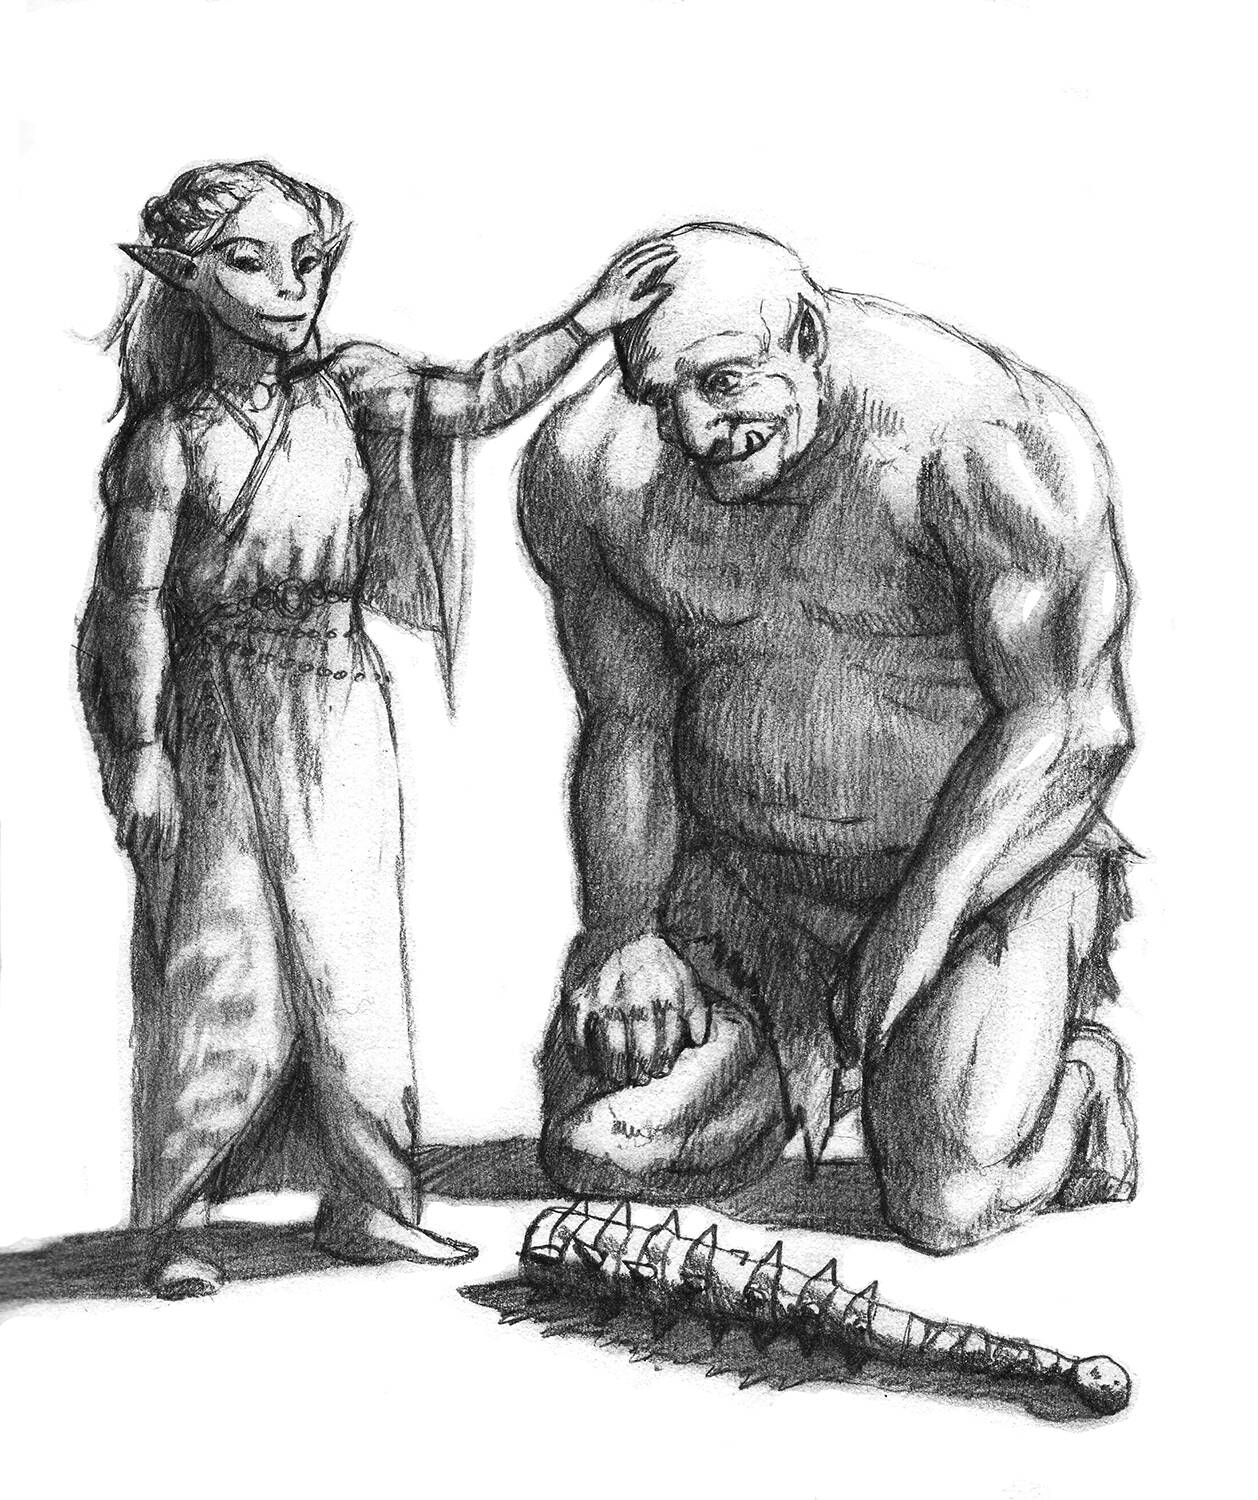
\includegraphics[width=.43\textwidth]{images/Roch_Hercka/elvish_enchanter.jpg}
	\end{wrapfigure}

}{}

The enchanter gives someone a particularly off-putting look and they immediately stops what is was doing, losing their train of thought. The target has trouble articulating what's wrong, but will remain confused for as long as the spell continues. The spell is sometimes initiated by eye contact, sometimes by song -- any number of social interactions can suffice for transferring the spell effects.

A resisted roll is made -- the enchanter uses their Intelligence + Deceit Skill while the target uses Wits + Vigilance. If the target loses the roll they immediately loses all remaining actions for the turn but can still defend them; the target's Initiative score instantly reduces to 0.

Each subsequent turn the target makes a resisted roll of\ Wits + Vigilance against the mage's Intelligence + Deceit. Failure indicates that they suffer an Initiative penalty equal to 2 plus the mage's Intelligence Bonus.

While the spell is in effect, the target suffers a penalty to all Mental Attributes equal to \arabic{spelllevel} plus the enchanter's Intelligence Bonus; so a mage with Intelligence +3 would inflict a -5 penalty. If the target attempted to cast spells, any rolls would suffer a -5 penalty and any spell-effects which relied on the Intelligence Attribute would suffer as well.

At the end of the scene, targets make one final resisted roll against the enchanter's Intelligence + Deceit (even if the enchanter is no longer present). Failure indicates that the target has forgotten the encounter entirely, including some moments before when the spell began.

If an \gls{npc} enchanter intends to cast this on a PC during a scene, the \gls{gm} is encouraged to simply make the resisted roll for the spell. If the player fails the roll then the \gls{gm} can infer what probably would have happened had the scene played out and skip to the next scene, telling the player that something important might have happened, but that they cannot remember any of it.

When this spell hits someone out of combat, perhaps during a conversation, targets tend to flap their mouths open and shut like a confused fish as they try to recapture their train of thought. The use of magic will is not obvious to those unfamiliar with such abilities.

\spell{Mind of Stone}{Continuous}{Empathy}
Enchanters of this level can also cast a greater version of Mind's Healing. The spell can cut the ill effects of any Enchantment spell and if cast as a casting spell the target becomes completely immune to unwanted Enchantment spells.

\spelllevel

The enchanter locks eyes or otherwise engages with the target and lulls them gently to sleep, forces them to repeat particular actions, or fills them with a dreadful fear. The target can reroll a failed resistance roll at the end of each scene.

\spell{Focus}{Continuous}{Empathy}
The target holds the last action performed and repeats it, again and again. If they were attacking, they will continue attacking until there are no targets left, and then go and look for some. If the target was attempting to mount a horse, they will chase it until they can no longer move.

The enchanter engages in a resisted roll of their Intelligence + Empathy versus the target's Wits + Vigilance. Targets can stop once their original action has become obviously impossible or is unmistakably complete.

\spell{Panic}{Continuous}{Deceit}
The enchanter and the target make a resisted roll; the caster adds their Intelligence Bonus and Deceit Skill while the target adds their Wits bonus and Combat Skill. If the target fails, they automatically run away in fear, as the enchanter dictates.

If the target would normally take a Morale check, the caster's Intelligence + Deceit are added to the \gls{tn} for as long as the spell is in effect. Targets completely unable to flee will continue to fight.

\spell{Rest}{Continuous}{Empathy}
Enchanters who want their target to fall asleep can make a resisted Intelligence + Empathy roll against the target's Wits + Vigilance. The target can spend 5 \gls{fp} to ignore the results of the spell. A successful spell means that the target has fallen asleep.

\spelllevel

\spell{Domination}{Continuous}{Deceit}
The target is given a simple command by the enchanter, consisting of no more words than \arabic{spelllevel} plus the enchanter's Intelligence + Deceit. If the target fails the resisted task of their Wits + Vigilance against the enchanter's Intelligence + Deceit then they must immediately obey any commands the enchanter gives them.

If the enchanter maintains the spell then the target can reroll at the beginning of each scene to break the spell again, otherwise it ends when the enchanter drops the spell.

	\begin{tcolorbox}[arc=1mm,tabularx={llp{.5\textwidth}}]
		Task Bonus & \gls{tn} & \\\hline

		Humiliation & +2 & Any action which would humiliate the target grants a +2 bonus to resist. \\

		Betrayal & +4 & Targets who would otherwise be weak-willed and at the mercy of the enchanter gain a +4 bonus to resist attacking their allies. This bonus can increase up to +6 to resist attacking loved ones such as family and close friends.\\

		Code Violation & Variable & Targets forced to act against their own code or god gain an additional bonus to act equal to the amount of \gls{xp} they would receive for completing the action. For example, those following the code of passion would gain 1\gls{xp} for trying a new type of food or drink, so they gain a +1 bonus to resist commands which inhibit their ability to act in this way. Those following Ohta, Goddess of War, gain 10\gls{xp} for bringing down a sufficiently large monster, so they would gain a +10 bonus to resist any enchantment which prohibits them from slaying such quarry. This can also be used against the target, with the enchanter gaining a bonus to affect someone with an order if it adheres to the target's code.\\

	\end{tcolorbox}

Giving a command can take some time, so in combat, Enchanters have to spend the usual 2 Initiative to speak in order to actually make a target do something, once the spell has been cast.

Some commands are easier to resist than others. Particularly repugnant commands allow the target to reroll to break the spell with a bonus.

\spell{Mental Illusion}{Continuous}{Varies}

The caster at this level can also create a mental illusion in the target's mind. The caster might look deeply into the target's eyes and force them to hear music which is not in fact there but persists despite all attempt to stop it. They might sing to all present about a dragon, and one particular listener will actually see, feel and smell that dragon.

In all cases a successful illusion will be complete, and the target will make every provision to interact realistically with the imaginary thing, be it a creature, an object or weather condition. It could even be something stranger, such as a box containing a spider's voice, or a statue of a sunrise which glows in unknown colours.

The caster and target make a resisted roll: the caster uses their Intelligence + some Skill relevant to the illusion being created. A caster making a dragon might use Ether Lore, while making an illusory cow would require Beast Ken. The target resists with their Wits and the same Skill as the caster.

The \gls{gm} should make this roll for players, in secret. The target gains a bonus to resist (or the caster takes a penalty) if the illusion is particularly unbelievable (such as a bizarre object or an unexplained dragon). Targets also gain a penalty to resist if they suspect that magic is being used to trick them, which often becomes obvious if lots of people around are insisting that rats are not in fact biting off their toes.

Such mental illusions can inflict up to 4 Fatigue Points plus the caster's Intelligence Bonus and multiple castings allow the Fatigue Points to stack up. These Fatigue Points are healed as normal. The player may be told that this is Damage, but the \gls{gm} should keep track of it separately to ensure that all the Damage is properly converted once the spell fails. Such Fatigue Points can kill a character in the usual manner, i.e. by giving the target a Fatigue Penalty beyond -5.

\spelllevel

\spell{Mental Bondage}{Continuous}{Deceit}
The enchanter locks down the target's every thought and turns everything they know to a desire to serve only the enchanter. They will follow any command to the best of their abilities, and if asked why will proclaim an unconditional love for or obedience to the caster.

The target makes a resisted task of their Wits + Vigilance against the enchanter's Intelligence + Deceit. Success (from the target's point of view) means that the target breaks the spell but failure (a successful roll on the part of the enchanter) means that the spell is fixed -- for as long as the caster wishes the target will serve them loyally. Immediate threats to the target's life, such as being told to jump off a cliff or being told to drink something by an enchanter who was previously trying to kill the target call for a reroll, but there is no automatic reroll at the beginning of each scene. This spell is subject to the same modifiers as the previous level.

Enchanters might use this to turn attacking ogres into a loyal group of warriors to use against other enemies, or simply to turn a favoured artist into a persistent plaything of the local court. This spell may be expensive in terms of \gls{mp} but over time the target may come to loyally serve the enchanter naturally, assimilating the spell into normal, everyday habits. Every month of service prompts a new roll -- success means that nothing happens while if the target fails they must serve the enchanter even after the spell has been cancelled, with full normal effects. Enchanters do not know when their spells have turned into long-term spells, but they can often guess by looking at just when the target has stopped trying to fight the spell.

If the enchanter ever dies, the target can reroll each scene to break the spell.

\spell{Tabula Rasa}{Continuous}{Deceit}

The target's memories can be filched -- either selectively or not. The caster specifies (through song, words, or a simple glance) which memories are to be removed. If a target loses access to a Skill due to this spell, they can no longer use it until the spell ends.

The caster uses their Intelligence + Deceit while the target resists with their Wits + Vigilance. Success means that the caster has free reign, not to rifle through the target's exact memories, but to specify that anything they wish is lost, up to and including all memories. The target always retains their first language.

\sphere{Fate}
\index{Magic!Fate}Fate deals with divine blessings and luck. At first the caster learns to ask questions of the gods, or to perhaps reach into an inner intuition about the world. Next up the mage learns to heal people's \gls{fp} and increase targets' average luck. Finally, priests can help bring people back from the edges of death.

\spelllevel

\spell{Curse}{Continuous \& Instant}{Deceit}
Additionally, casters can curse a target. The target loses $1D6$ \gls{fp} plus the caster's Intelligence Bonus. If the target has no \gls{fp} then this spell has no effect. The mage is allowed to know how many \gls{fp} the target has lost. The target cannot dodge in any way -- the caster simply rolls their Intelligence + Deceit against \gls{tn} 7.

If cast as a standing spell, the target's \gls{fp} are reduced by 1 plus the mage's Intelligence Bonus for as long as the spell endures.

\spell{Eyes of Fate}{Continuous}{Empathy}
The priest prays for guidance, gains a keen insight into the fate of others.

Once the spell is cast, the priest knows the current \gls{fp} of everyone within the normal spell range.

\spell{Intuition}{Instant}{Varies}
When players search for an item, or ask around town for someone's whereabouts, the \gls{gm} often won't tell them the \gls{tn}.  With this spell, the priest may demand to know the \gls{tn}.  The Skill used is the same as that being used in the task, so asking about a roll for Crafts means using the Crafts Skill for the spell.

\spell{Lending Hand}{Continuous}{Empathy}
The priest blesses a target with +1 to any Skill, so long as the priest has a higher level than the target in that Skill.

\spelllevel

\spell{Auguary}{Instant}{Academics}

The character requests guidance about the future and receives a cryptic message from their deity, from dreams, or simply the shape of nearby clouds.

Once cast, the \gls{gm} looks through the upcoming encounters and picks a description.  It could be random boxtext, a note about an upcoming character, or a metaphor involving upcoming events.  A good rule of thumb would be to give the caster information about closer encounters with a better Margin on the roll.  A roll reaching the basic \gls{tn} of 7 might give the priest information about something three encounters away, while a roll of 11 could tell the caster about the very next encounter.

Characters who continue to cast Auguary receive the same answer each time until they have run into the encounter, or somehow bypassed it.

Nobody in Fenestra ever says ``you cannot change your fate''.  Changing your fate is the entire point of this spell.  Besides, if the spell ever appears to go wrong, the local priests will explain that it actually predicted events correctly.  It was simply your knowledge of the spell that -- somehow or other -- altered what would otherwise have been a fine prediction.

\spell{Pious Favour}{Instant}{Academics}
The priest blesses the target with the favour of the gods. The target `heals' or regenerates $1D6$ \gls{fp} plus the priest's Intelligence Bonus. This cannot take the target above their maximum \gls{fp} score.

\enhancement{1}{Chosen}

The priest heals the target for an additional 2 \gls{fp}.  These \gls{fp} stack just like Damage, so $1D6+4$ \gls{fp} becomes $2D6$ \gls{fp}.

\spelllevel
\spell{Blessings}{Continuous}{Empathy}

The priest blesses a target, who then receives a +1 to any Skill.

\spell{Prayer of Gratitude}{Instant}{Academics}
The caster rolls during any scene in which someone spends at least 2 Story Points.  With a successful roll, one Story Point is returned to the character.

\spelllevel

\spell{God's Chosen}{Continuous}{Academics}

The target increases their maximum Fate Points by 10 and instantly heals a number of Fate Points equal to $2D6$ plus the caster's Intelligence Bonus. When the spell ends, the maximum FP return to normal. The spell does not increase the rate at which FP are regenerated.

\spelllevel

\spell{Divine Favour}{Instant}{Academics}

The priest spends 1 Story Point and gains an addtional 5 Story Points plus their Intelligence Bonus, which must be spent immediately.  This can be used on a summoning miraculous help, such as a crew of soldiers who have a debt to the priest, or a magical ally.\footnote{As usual \gls{gm} is free to veto any ideas, but the player is also allowed to continue pulling new ideas out.}

\spell{Resurrection}{Instant}{Medicine}

The priest summons the soul of a recently deceased person back to their body. If they are beyond -3 Hit Points, they must roll a Vitality Check again to stay alive, but this time with a +5 bonus. There is no roll for the caster -- the spell is automatic and the spell is instant, so the effects need not be maintained. If the spell is made into a standing spell then the effects count as being continuously cast.

The spell also heals the target of a number of HP equal to half the Margin. This cannot bring the target above 0 HP. For example, if a PC were at -7 HP they would normally make a Vitality Check at \gls{tn} 11. Adding in the Bonus would make the adjusted \gls{tn} 6. If the Vitality Check were a roll of 11 then the Margin would be 5 and the character would heal 3 HP, going up to -4 HP. This healing should be understood as a retroactive blessing from the gods, indicating that the Damage sustained was not nearly so bad as was once thought.

The spell must be cast within the same scene as the target lost their last HP.

If cast on a member of the undead, the target loses $2D6$ \gls{hp} plus the caster's Intelligence Bonus No roll is made, and no protection can be given from \gls{fp}, \gls{SP} or any other source.

\spell{Mana Lake}{Continuous}{Empathy}

The priest sanctifies and area, creating a mana lake.  The level of the mana lake is equal to the number of Story Points the priest spends.


\iftoggle{verbose}{

\begin{exampletext}

	It was some time before the group reconvened. They had to be confident no nura were waiting in the area. A clever search party might have left some people behind to wait and listen for movement, but the hobgoblins had left all their dwarvish cunning behind when they were transformed into nura.

`Whar the feck are we? Ah cannae see doon tae anywhere', Hugi muttered.

`Nor I', said Thenton, disappointed. `There is mist or cloud everywhere. We have come off course and had very little idea of our original course besides. We have lost all opportunity to ask friendly dwarves for help. By the time we get down safely we might have gotten farther off course and the village we were headed for on the other side may be well out of reach'. He sighed, and his warm breath mixed in with the surrounding clouds like drips of water on the ocean.

`It is time for the runes' stated Hugi.

	The \gls{gm} determines that the task's \gls{tn} is 6. Like all magic, rune casting uses the Intelligence Bonus. Hugi's Intelligence is +1, as his his Academics Skill, but his Fatigue penalty is -2. He rolls without bonus or penalty and gets a final score of 7: a pass. The runes inform him which direction to travel to catch their man. Finally, he marks off a single Mana Point for the cost of the spell.

'The runes say we gang doon thar', Hugi pointed into an apparently random path quickly being swallowed in mist. `Lemme gi' yous a blessin'. Gither roon'

Hugi intends to give his troops a blessing. No roll is involved, so he does not need to worry about the Fatigue Penalty. It is only when his player marks off the last 2 \gls{mp} that he realises that only one person can effectively receive the blessing. He rolls $1D6+1$ and heals Arneson for 4 FP, giving him 8 out of 11 FP.

\end{exampletext}
	}{}

\sphere{Force}\index{Force}

The mage can shape pure energy, pushing and pulling at the world with the power of their will alone. They can form shields, pick up weapons and grind targets into the ground as if with an invisible, giant, floating hand.

The force sphere does not come with discrete spells at each level. Instead, the mage gains access to all spells immediately. Each spell can be cast at any level the caster possesses, so a mage with the 3rd level of the force sphere could cast `Mage Armour' at level 1, 2 or 3 -- each with increasingly more expensive cost and a better shielding.

\spell{Mage Armour}{Continuous}{Academics}

The mage casts a shield of crackling energy around the target to protect from all harm, and most often mages target themselves.  The barrier can shatter if attacked but can take a serious beating before breaking. Each barrier counts as a having a number of \index{Shield Points}\gls{SP}, which are destroyed by Damage like \gls{fp}, but always before \gls{fp} are targeted. The target gains a number of \gls{SP} equal to the level of spell used times 3 plus their Intelligence bonus.

Those protected by the shield cannot attack others as the shield stops all attacks.  Casters are able to focus enough to use missile weapons and spells.\footnote{Allowing a target to use a missile weapon requies complete focus, and a Wits + Empathy roll.}

For example, Annabel the alchemist has the force sphere at level 3 and Intelligence +2. She's low on \gls{mp} so she casts it at level 2, gaining 8 \gls{SP}. On the very next Initiative Count she's hit for 10 Damage and loses all 8 \gls{SP} then 2 FP.

The spell must be maintained as a standing spell to function. Multiple castings do not stack -- only the highest casting it used. The shield can be placed on others if need be, not only the mage.

Armour does not block Damage going onto \gls{SP} -- the character simply subtracts \gls{SP} without any \gls{dr}. The Mage Armour is not affected by a Vitals Shot -- it protects all around, counting as Perfect armour, although not quite continuously enough to keep out water or gasses. Multiples of such spells do not stack -- only the highest is used.

\spell{Mage Sight}{Continuous}{Vigilance}

The mage can `feel' by delicately touching things with mental movement rather than actually seeing them. They can see in complete darkness whether underwater or on land.

The mage rolls Intelligence and Vigilance at \gls{tn} 6 plus the spell's level. The spell covers a progressively larger area depending upon the level used. No roll is required -- the spell is automatic and lasts until dispelled.

\vspace{.3cm}

\begin{tcolorbox}[arc=1mm,tabularx={ll}]

	Level & Radius of Sight \\\hline

	1 & 5 squares plus the caster's Wits. \\

	2 & 10 squares plus the caster's Force sphere rating plus Wits. \\

	3 & The entire \emph{area}. \\

	4 & 1 full area, up to 1 area away. \\

	5 & Five full sequential areas plus the caster's Wits. \\

\end{tcolorbox}

\noindent Mages able to perceive events multiple areas away make for legendary spies.

The mage's sight works a little like a floating, insubstantial eye which is unaffected by darkness or mist. It cannot go through walls and cannot see colour but can move at the speed of thought through a massive space and allows the mage a clear idea of the entire area. Smaller spells work as well as eyesight, while larger spells can be more difficult to use to track a full area -- most mages simply are not equipped to receive sense data from a full mile all at once.

Mages using Metamagic to increase the range of their spell can use this to sense things from afar. Someone using Metamagic to cast a level 5 Mage Sight spell would be able to see perhaps 7 areas at the same time, and cast spells with any one of them.

This spell allows people to perceive movement only, and not to hear what is happening in that location.

\spell{Dancing Swords}{Continuous}{Combat}

The force mage can make a weapon levitate with the power of their mind. It can float nearby to defend them and even float off to stab at enemies who will be hard pushed to counterattack the wielder when they're standing some distance away.

The caster rolls Intelligence + Combat to levitate the weapon. They gain an effective Strength Bonus for the purposes of wielding the weapon equal to the level of the force sphere being used minus one. This must be sufficient to lift the weapon without encumbrance, so a mage casting the first level of the force sphere would have an effective Strength Bonus of 0 and could wield a dagger. To wield an axe a mage would have to use the fourth level of the force sphere, gaining an effective Strength Bonus of +3.

While the weapon is next to the caster it can defend them just as any weapon. An axe would add +1 to the caster's Evasion Bonus while a long sword would add +3 to the caster's Evasion total. The weapon can add this defence to anyone nearby but only one person at a time.

To attack with the weapon, the mage spends the normal amount of Initiative for that weapon; e.g. 4 for a dagger and 6 for a shortsword. They roll with Intelligence + Combat and deals the normal amount of Damage given the effective Strength Bonus, so a fourth level force sphere spell could wield a dagger to deal $2D6$ Damage, or could wield an axe to deal $2D6+2$ Damage.

If the mage levitates multiple weapons (through multiple castings), each additional one adds +1 to their Strike score, adds +1 Damage and +1 to the Evasion Bonus. In this way the mage can add up to a maximum of +3 to each stat, meaning only the first four weapons can have an effect. Additional weapons can add Evasion Bonuses behind or to the side of the mage to ensure they do not lose any Evasion Bonus when attacked from behind but a fifth weapon cannot add additional Damage.

If someone wants to grab one of the floating weapons they must roll with their Strike Factor just as when making a grab against any character. The mage defends with their normal Evasion Factor and a successful grab means that the weapon has been arrested. The weapon gains a Weight Rating equal to the Weight of the character grabbing the weapon (which is equal to their maximum HP). At this point the weapon is too heavy to lift and the spell ends.

The levitated weapons do not add a Speed Bonus to the caster's Initiative -- they must use their Wits Bonus as usual.

The caster may not employ any special combat manoeuvres such as pushing people back or fighting in the Aggressive Stance. No Knacks concerned with Combat apply to the mage wielding this weapon.

\spell{Levitation}{Continuous}{Combat/ Craft}

This is a more generic version of `Dancing Swords' (above) where the mage can lift but not necessarily weaponize anything close by. The caster rolls their Intelligence and Craft Skill against a \gls{tn} of 7 plus the target's Weight Rating. The spell grants an effective Strength Bonus equal to the level in the force sphere being used. Any object with a Weight Rating of up to 4 points higher than this Strength score can be lifted into the air but the heavier something is the slower it will move.

If creatures are targeted for levitation, they have a Weight Rating equal to their HP and the mage rolls Intelligence + Combat to lift them. They can add their Evasion Factor to the spell's \gls{tn} in order to attempt to wriggle free of the telekinetic hold. Trying to wriggle free takes 4 Initiative points. Targets can be moved at a Speed rating equal to the level in Force.

Mages attempting to lift people into the air can move the target only at the rate of a standard action -- i.e. 3 squares per turn plus their effective Speed rating. The effective Speed rating is equal to the spell's level, but the spell can be encumbered just like lifting a normal person. So casting a spell at level 3 means an effective Strength and Speed rating of 3; if the target had Strength +1 they would have 7 HP and therefore a Weight Rating of 7. That's 4 points above the spell's rating so the Speed suffers a -4 encumbrance penalty, making the total movement 1 square every two \glspl{round}. The target could roll to be free every 4 Initiative steps, rolling against the spell's effective Strength Bonus.

While a target is being levitated, they are especially vulnerable to attack, and all attacks against them count as Unseen Attacks, gaining +4 to Strike and +2 to Damage.

\spell{Lock}{Continuous}{Craft}

The mage can erect a magical force field, similar to mage armour, over a doorway to make it more difficult to break through. The \gls{tn} to break through the door increases by an amount equal to double the level of the force sphere being employed plus the mage's Intelligence Bonus. For example, if a door were at \gls{tn} 8 to burst through, a mage with Intelligence +2 could cast the second level of the force sphere, raising the \gls{tn} to 14.

Mages can also create barriers of pure force to block passageways without a door, just as with mage armour. The blockade has a number of \gls{SP} equal to triple the level of force sphere being employed plus the mage's Intelligence Bonus and must be battered through with repeated blows to get through the portal.

\spell{Slow Fall}{Continuous \& Instant}{Athletics}

When people (or even items) are falling to their doom, force mages can slow the decent, limiting the Damage from such a fall. The total spell grants a resistance to any Damage incurred through falling equal to 4 points per level of the force sphere used plus the mage's Intelligence score. Therefore, a mage with Intelligence +2 using the third level of the force sphere would subtract 14 from any Damage incurred through falling.

If cast as an Instant spell, this ability subtracts from all falling Damage when needed. If cast as a Quick Spell, it can be cast as a Quick Action, outside the usual Initiative order.

\spell{Telekinetic Fist}{Continuous}{Combat}

The mage uses powerful telekinetic blasts to hold and crumple targets in close combat. Unarmed attacks using Telekinetic fist count as normal Damage instead of inflicting Fatigue Points. For the purposes of these attacks, the caster counts as having a Strength Bonus equal to the level of the force sphere being used. For example, someone employing the third level of the force sphere would count as having +3 Strength, and would inflict $1D6+3$ Damage with unarmed attacks.

\spell{Telekinetic Grasp}{Continuous}{Combat}

Force mages can wrestle with people from afar using telekinesis. One major advantage with this sort of wrestling is that the mage does not risk being hit back as they can cast the spell from afar. As per the Grappling rules, the mage first makes a roll to capture the target; they roll Intelligence and Combat while the target resists with their current Evasion Factor. Targets can literally feel the force of the mage's mind around them, often described as a hundred tiny, invisible hands or the feeling of an invisible wave. This force can be parried and pushed back like any normal weapon, so targets can use their full Evasion Factor, including bonuses from using a weapon.

If the spell is successful, it inflicts no Damage nor Fatigue Points, but the target counts as carrying an item with a Weight Rating equal to the level of the force sphere being used.

For example, a mage using force level 2, with Intelligence +1 and a Combat Skill of +1, could cast Telekinetic Grasp on a gnome. The gnome adds their Evasion Factor to the basic \gls{tn} of 7 and then the mage resists this with their Intelligence Bonus plus Combat Skill. If successful, the gnome would count as carrying an item with a Weight Rating of 2. Assuming this gnome has the usual Strength Bonus of -2, they would then receive a -4 penalty to their effective Speed Bonus. Their Initiative Score would suffer and they would accrue additional Fatigue Points each time they attempted to run or fight due to the added Weight Rating.

\spell{Telekinetic Retreat}{Continuous}{Athletics}

Mages can add their mental ability to move things to aid their movement. Any attempts to move, whether fleeing or just flitting around a room, gain a bonus equal to the level of the force sphere being employed plus their Intelligence Bonus. The mage can cast the spell on others and it will automatically push them onwards in whichever direction they are running.

\sphere{Illusion}\index{Illusion}

Illusions create a facsimile of sounds and sights out of pure magic. The thing created might look like a hat, a coin, a rat or even a dragon at higher levels. Illusions also create convincing sound -- loud echoes, the sound of nearby battle, perhaps even imitating an enemy commander's orders in battle. However, illusions are little more than coloured air and noise -- once touched they fade away. They are frightening and if properly used can defeat armies, but are not perfect weapons by any means.

Seeing through an illusion is always an opposed roll -- the illusionist adds their Intelligence Bonus while anyone seeing or hearing the illusion resists with Wits + Vigilance. The \gls{gm} should roll in secret if an illusion is present, and inform the players of the deceit if the players spot it. If someone has a reason to suspect that something is an illusion, they should receive a +2 bonus to resist it. The party also receive a bonus for multiple people who might spot the illusion, as per the standard Vigilance Skill rules.

Illusionists add different Skills to the roll, depending upon what they are making an illusion of. An illusion of a cart or sword might require the Craft Skill. An illusion of a monster might use the Academics Skill. Specialisations in the correct area are, as usual, a requirement if the caster wants to avoid the usual -1 penalty for lacking the appropriate specialisation.

For example, a gnome creates an illusion of a fleeing gnoll with a great bundle of treasure in his hand, hoping the PCs will chase after him immediately. His Intelligence is +2 and his Academics is at +1 though he has no appropriate specialisations, so the players are rolling at \gls{tn} 9. The \gls{gm} takes the party member with the highest Wits + Vigilance who has a score of +3 in total. The next highest score in the party is +1 but nobody else has anything. The total is +4 so the \gls{gm} rolls for them and obtains a total of 8 -- that's not enough. As they begin to run, one of the PCs remembers they heard about a gnomish illusionist and asks `Are we chasing an illusion?' - that puts that final score up to 10; the \gls{tn} is reached and the \gls{gm} informs the player that she sees that the gnoll's feet are not always touching the ground properly, so it must be an illusion.

The \gls{gm} should grant bonuses and penalties to illusions depending upon lighting conditions -- illusions inside a shadowy cottage seen from far away should receive an immense bonus, while far-fetched illusions on a sunny day seen up close might receive a penalty.

Illusionists typically create images of things they are familiar with. Unfamiliar objects, such as an illusionist trying to recreate a dragon while never having seen a dragon, suffer a -2 penalty to the roll, at minimum.

While most people are aware that illusion magic exists and so are suspicious of anything outlandish or out of the ordinary, those who have never heard about illusory magics suffer a -2 penalty to disbelieve.

If someone sees an illusion for what it is then the illusion remains, but of course will have less effect. However, while someone fully believes an illusion to be real, they can be psychosomatically damaged by it simply by believing that it's real. All illusions can inflict a total of 1 Fatigue Point per level of the illusion spell plus one per Intelligence Bonus of the caster. For example, a song mage might sing a griffin illusion into existence; all who are fooled by the illusion can be `attacked' by it, receiving up to 4 Fatigue Points. On later \glspl{round} the song causes no more Fatigue Points, even if it keeps playing, but the bard could then create the illusion of a sword using the first level of the illusion sphere. They could use the sword to attack as usual, but not parry blows. While attacking, they could inflict up to 2 Fatigue Points as people believe they have been wounded by the sword, but subsequent attacks would not increase the amount of Damage.

Illusions must be summoned within the normal range of spells, but once summoned they can travel away from the caster without worry -- so long as they are maintained as static spells, they endure, no matter how far away the caster might be.

\spelllevel

\spell{Illusion}{Continuous}{Varies}

The illusionist can make anything look like another of roughly the same size.  A fox can look like a dog, a copper coin can look golden, or a gnome can appear like a gnoll.

Illusionists can use this to hide by making themselves look like a bush, or slip unseen into a party by making themselves look like one of the other guests.

Copying a person requires the Empathy skill, while copying furniture would require the Crafts skill.

Anyone touching an illusion finds that it melts in their hands -- a simple handshake can shatter a basic illusion, and handling fake coins quickly dissipates the magic.

Illusionists cover both sound and appearance.  Illusions crafted for sound can change a nearby river to sound like howling wolves, or make someone's voice come out high-pitched.

Illusionists who speak another language can make someone else's speech sound like that language.  If you speak gnomish, your colleagues can be made to sound like they speak gnomish.  Another spell could make a number of gnomes sound like they're speaking in the common tongue.  \footnote{Of course at that point, everyone would understand each other, but have a hard time understanding themselves.}

Seeing through an illusion requires a Wits + Vigilance roll, with a \gls{tn} equal to 7 plus the caster's Intelligence and skill (whatever it happens to be).  Alternatively, when a player rolls for an illusion, the \gls{tn} is 7 plus an opponent's Wits + Vigilance.  Having multiple \glspl{tn} can mean some opponents are fooled and some are not.  Anyone specifically looking out for an illusion can gain a +2 Bonus on the roll, or a +4 if they have reason to suspect that the thing in front of them is an illusion.

Illusions require a caste's full focus in order to remain realistic.  A caster who make his friend look like an elf would have to pay attention to his friend to make sure the facial movements followed along.  Casters cannot engage in anything more than simple conversation or walking while maintaining illusions.

Illusions can only adjust something's size so much.  Something's weight rating can increase or decrease by a number equal to the spell level plus the caster's Intelligence.  A first level Illusion spell cast with Intelligence +1 could make an elf look like a gnoll, but could not make a gnome look like an ogre.  Similarly, a shortsword could be made to look like a simple dagger, but turning a chainmail suit into a small bird would extremely difficult.

\enhancement{1}{Independent}

Illusions can now be cast without any `base' -- they simply appear on their own.  Coins, dogs, dragons, or more, can be fashioned from nothing.  Independent illusions can continue acting in an intelligent manner without any intervention from the caster.   People's speech can be adjusted to another language long after the illusionist has left, or a rock made to look like a human soldier could continue moving and speaking 

\enhancement{1}{Large}

The illusion can now cover a large area; specifically it can cover a number of squares equal to the spell's level plus the caster's Wits Bonus.

Audio spells become deafening, and cover an entire area.

\enhancement{1}{Solid}

Solid illusions are not all that solid, but they can be touched without disipating.  They are also far more realistic, and increase the \gls{tn} to see through the illusion by 2.

These illusions have a Strength score equal to -5, plus the spell's level, plus the caster's Intelligence and skill.

Solid illusions become an extension of the caster, and any caster can cast a spell \textit{through} the illusion, as if the illusion were the caster.  This might be used to cast an Invocation spell through a dragon illusion, or could employ Force to help an illusory creature lift a sword.

Once even a single point of Damage has been dealt to the illusion, it vanishes.

\enhancement{2}{Massive}

Massive Illusions cover an entire area.  Powerful illusionists can make everyone in a castle's wing look like goblins, or make a filthy kitchen appear clean.

\enhancement{2}{Negative}

The illusionist finally learns to make less of something, rather than more.  A single person can be silenced, or made invisible (or both).

As usual, the illusion is still delicate, and if the person is struck or disturbed in any way, the illusion dissipates.  Combat rolls, for defence or attack, always break such spells unless they are also make \textit{Solid}.

\sphere{Invocation}\index{Invocation}

This is the first choice of spheres for a battle-mage. It is designed specifically to destroy targets with balls of lightning and fire. It also has more subtle uses as casters can extinguish flames, plunging people into darkness.

Armour functions as normal with Invocation, though like any other projectile bolts of fire can attain a Vitals Shot (see page \pageref{vitals}) and bypass armour entirely.

All Invocation spells are rolled as Projectiles, using the mage's Intelligence Bonus and their Projectiles Skill; casters must have a Projectiles specialisation in invocation or receive a -1 penalty to all spells. The basic \gls{tn} is 7 and the difficulty raises by +1 for every 5 squares away the opponent is, just as with normal missile weapons. As usual, opponents who are keeping edgy (see page \pageref{edgy}) can use their Speed to resist the attack, adding it to the \gls{tn}. Alternatively, if a player is keeping edgy, it is they who can attempt to dodge the incoming attack, rolling their Speed at \gls{tn} 7 plus the pyromancer's Intelligence and Projectiles Skill. Shields' Evasion Bonus can add to the roll to resist such spells.

Just like any other long-range spell, Lightning Bolts and other Invocation spells can succeed in Vitals Shot, bypassing armour, if they strike precisely enough (see page \pageref{vitals}). Blast-radius spells such as Fireball can inflict a Vitals Shot on up to 1 person, specified by the caster, but not more as the mage cannot make precise attacks against a group of people simultaneously.

If you are using miniatures, it will be easy to see how many people are caught in the blast radius of a spell. The caster can direct which squares are affected so long as they are all joined together; they may be squares forming a larger square, or spread out in a row. However, if your group is more a fan of the mind's eye theatre the assume that for every square in a spell's range has it affects 1 target.

\spelllevel

\spell{Lightning Bolt}{Instant}{Projectiles}

The mage throws out a ball of flaming, crackling light which strikes and burns the target. The Damage is $1D6$ plus the caster's Intelligence.

\subsubsection{Spell Enhancements}

\enhancement{1}{Inferno} The caster increases the spell's level by one and increases the spell's Damage by 2.  A mage with Intelligence +2, casting Lightning Bolt at third level would deal $2D6+2$ Damage.

\enhancement{1}{Fireball} The caster turns the lightning bolt into a raging fireball, which covers a number of squares equal to the spell's level plus the caster's Wits.

Anyone within 1 square's distance of the fireball takes 1 Damage plus the caster's Intelligence Bonus.

\enhancement{2}{Inner Furnace} The pyromancer finally learns how to summon fire upon a target without throwing it -- no ball of flame is thrown, fire simply appears, surrounding the target and instantly covers a target anywhere within normal range. It seeps into soft spots and gets into the chinks in armour, bypassing \gls{dr} entirely, including Perfect armour such as \gls{SP} from Mage Armour. The target cannot resist in any way.

\enhancement{2}{Eternal Flame} The fire cast does not go out unless plunged under water.  Each round it continues to burn, inflicting $1D6$ Damage plus the caster's Intelligence Bonus.

If the spell targeted an area with the Fireball enhancement, the area burns, rather than specific people or items inside.

If the spell does not have the Inner Furnce enhancement, it always targets people's outer layers; their swords, armour, clothing, but not the person themselves, unless that person was mostly naked.

\sphere{Metamagic}

\index{Metamagic}

Metamagic allows the \gls{miracleworker} to enhance their other magic spheres -- adding to their range, casting more spells in a \gls{round}, gaining more \gls{mp} to power them and eventually includes the ability to create magical items.

Casting a metamagic spell \emph{adds} to an existing spell's level.  A Fireball spell is 2nd level, so it would usually cost 2 \gls{mp} and an additional 2 Initiative, but if the first level of Metamagic enhances the spell, the cost would be 3 \gls{mp} and 3 Initiative.

Metamagic never increases the static cost of a spell.  If the caster makes an illusion, and casts it over many targets by using Metamagic, the spell can be maintained with the original cost of the illusion -- the additional Metamagic points do not have to be maintained.

\spelllevel

\spell{Counterspell}{Continuous}{Sphere Rating}

The caster binds another caster's magic, disrupting the flow of mana.  Any time the opposing caster attempts a spell, the \gls{tn} is increased by the caster's Intelligence plus the caster's rating in the appropriate sphere.  For example, if the target attempts to use Necromancy, but the caster has level 1 Necromancy and Intelligence +2, the target would suffer a -3 penalty.

Counterspell magic works even when the caster has a rating of 0 in the appropriate sphere, although only the caster's Intelligence Bonus has any effect.

\spell{Detect Mana}{Instant}{Empathy}

The mage casts the spell on any person or item and finds out how many \glsentrylongpl{mp} the target has, including any mana stones the target has.

\spell{Spell Breaking}{Instant}{Sphere Rating}

The caster can destroy an existing spell, whether that spell is a persistent effect, such as a polymorph, or a magical item.  The \gls{tn} is the highest Sphere level used plus the Intelligence Bonus of the \gls{miracleworker} who cast the original spell.

For instance, if a priest with Intelligence +1 and Aldaron +3 were to cast a spell enchanting an animal, the \gls{tn} would be ($7+3+1=1$) 10.  The caster would roll using Intelligence plus their rating in the Aldaron sphere.

\spell{Spell Throwing}{Instant}{None}

Throwing a spell means that the normal range boundaries can be ignored -- spells can be thrown anywhere. Of course, the target must usually be seen -- there's no use casting a flame bolt into the darkness of a forest and specifying the target as `any nearby enemies'.  However, the caster is always free to guess.

\spell{Mana Stones}{Continuous}{Academics}

Each Path of Magic has its own version of mana stones. Once an item (or creature) is designated as a mana stone, the spell is cast and the mage forfeits any number of \gls{mp} from their maximum. For each \gls{mp} forfeited, the mage can store 2 \gls{mp} in the stone. These stones always start life empty, but regenerate 2 \gls{mp} per scene until they reach their maximum. Anyone on the same Path of Magic can retrieve the mana from the stone by simply touching it. The spell is always permanent -- no additional mana must be kept aside so that the spell remains active. Retrieving the mana takes the normal amount of time to use an item -- 8 Initiative points

The mana in mana stones cannot be used to create more mana stones and mages cannot enter their own temporary \gls{mp} into the mana stone.

Mana stones form the basis of all magical items, and \glspl{miracleworker} can only use their traditional mana stones to create magical items.

\spelllevel

\spell{Pocket Spell}{Continuous}{Crafts}

The caster changes the basic nature of a mana stone so that it can contain one spell.  A single \gls{mp} is stripped from the mana stone, after which it can cast a single spell, just once, before becoming useless.

Some mages create scrolls which are destroyed once read.  Some priests of Laique enchant animals with a single spell, just to see how the animal will use it.  The only limitation is that the mana stone must have enough \gls{mp} to cast the spell once.

The pocket spell always produces a single effect and any continuous effects last until the end of the scene.  The mage can create an item which casts an illusion of a dragon, but never a scroll where the user determines the illusion cast.

These magical items are activated by a `command word'. Command words do not necessarily have to be actual words -- they could be entire phrases or gestures. Importantly, when activating an item people must spend the usual 8 Initiative points for using an item, because some concentration is always required.\footnote{Knacks cannot reduce this cost.} Magical items which cast a continuous spell always come with a second command word to stop them.

\enhancement{2}{Mirror Magic}

This metamagic enhancement allows \emph{any} spell be be doubled at the cost of raising it by 2 levels.  A fireball could turn into two fireballs.  An illusion could disguise two people instead of one.

In each case the spell must have different targets, because two copies targeting the same person, would just result in one spell.

\spelllevel

\spell{Magical Item}{Continuous}{Academics}

The mage takes a mana stone and allows it to cast a spell, forging a new magical item. A sword could be made which can summon blinding light, or a ruby could be infused with the power to teleport the caster to a nearby location.

To implant a basic spell the mage casts the Magical Item spell, expending \arabic{spelllevel} \gls{mp} as usual, which then lowers the maximum \gls{mp} of the item by 1. After this the item can cast just that spell with its own \gls{mp}. For example, imagine a painting which casts an illusion of the person in the painting walking out and speaking with people any time the command word is uttered. If the item had 6 \gls{mp} then it would reduce to 5 \gls{mp} and would spend 3 of that 5 \gls{mp} in order to cast the spell. These magical items regenerate \gls{mp} in the same way as above (usually, 2 \gls{mp} per scene). Magical items are still mana stones and continue to store \gls{mp} for use by people on that Path of Magic.

Such basic spells always take effect in exactly the same way and use the mage's stats for any rolls. A second level aldaron spell set to freeze water will always do just that, and can never cast a Sunray. An illusion-generating mask, making the wearer into a bush, will always turn that wearer into a bush, regardless of what the user may want the illusion to be of.

Magical items which do not have enough mana simply fail to cast. The one exception here is the Path of Song, wherein spell-songs which have too much mana drawn from them simply break.

\spelllevel

\spell{Greater Item}{Instant}{Academics}

The mage can now input any number of spells into an item, and each additional spell again only requires that 1 \gls{mp} be stripped from a mana stone.  Spells so imbued can be cast any way the caster wishes -- an illusion spell in an item can be used to cast any illusion, or a polymorph spell can be used to turn into any creature.

The spell lasts until a second command word is given to release the spell.

\spell{Spell Triggering}{Instant}{Academics}

The mage takes a magical item with spells implanted and changes the spells there so that it activates upon a condition, and does not require concentration or focus.

A sword might throw out a flamebolt spell when it strikes a target.  A ring could cast an illusion of anything the mage says.  A priest who worships V\'{e}r\"{e} could imbue a holy warrior with a spell which adds to the warrior's \gls{fp} any time they receive damage.-- any trigger is possible so long as the trigger is clearly visible to the item.

Additional spells may be placed on items which are there simply to act as a trigger.  A Fate spell might detect incoming danger and cast an illusion as a warning, or a Detect Mana spell could immeidately raise any nearby dead as ghouls if some new magical effect is in the area.

\enhancement{2}{Spell Forking}

\emph{Any} spell, whether Metamagic or otherwise, can now be cast at two levels higher, and gets a number of copies equal to the spell's level plus the mage's Wits.

As with the Mirror enhancement, above, each spell must select a different target.

\spell{Artefact}{Instant}{Academics}

This spell functions as per level 3's Magical Item spell except the magical items are not activated by focus and concentration. Instead, each implanted spell can activate once per scene when a condition is present. The artefact might activate to shoot a flame-bolt any time a human is within range, or a magical ring could transform the wearer into a bat (if possible). The item requires no Initiative expenditure to use and cannot be switched on and off at will.

Such items also come with their own cancellation conditions. Permanent spells such as raising the living dead cannot be cancelled, but a levitation spell from the Force Sphere might activate and deactivate with the speaking of a particular word, or a spell to turn the wearer of a cape invisible might cancel once they have killed someone.

In all cases the condition must be clearly present -- items do not have magical abilities to detect special conditions such as `when a hidden enemy is present' unless the item is given access to spells which can find that information out..

Those on the Path of Song can infuse spell-songs which activate on their own once sung in addition to other effect. The effects of the artefact song would then not require additional Initiative expenditure above just singing a song, perhaps to activate another spell.

\spelllevel

\spell{Improved Mana Stones}{Instant}{Academics}

The mage's mana stones now contain 3 \gls{mp} per point sacrificed from the mage's permanent maximum, so sacrificing 3 \gls{mp} would yield an item which can store 9 \gls{mp}. These stones regenerate 3 \gls{mp} per \gls{round}.

\sphere{Necromancy}\index{Necromancy}

Necromancers summon souls from distant, black realms and place them in appropriate bodies -- those of the once living and now dead. The corpses are sometimes filled with their old hosts, locking people into a state of permanent semi-death, or more often with ravenous and malicious spirits from foreign realms. Mages of this sphere begin by imitating the dead, becoming half dead themselves, which allows them to dissuade malicious spirits from attacking.

\spell{Properties of the Dead}{undead creatures have certain properties in common. Firstly}{imperceptibly feed from the souls of the living. This is not performed with the mouth by merely by being close to dying things and absorbing them before they can wander to the next realm. Undead eyes generally do not work, instead they `see' the souls of people shining outward. Inanimate objects such as books, or even fellow undead, are not so clearly seen; the undead can avoid bumping into these objects but have great trouble reading anything or working fine machinery. However, they can operate in complete darkness and even fight without penalty, using the light of living people's souls to see them. They can also see living beings from a great distance due to the soul-light they emit.}

Undead also feel no pain and suffer little from scrapes and bruises. As a result, they automatically have a \gls{dr} of 2 which is cumulative with armour. This counts as Complete armour, but not Perfect -- shots through their eyes or attacks which sever muscles still debilitate them.

The undead do not tire -- they take no Fatigue Points. They can walk or dig or fight endlessly, without tiring. They enjoy feeding on souls, but it is not required for them to continue moving. Each has an Aggression score of +2.

\spelllevel

\spell{Deathly}{Continuous}{Medicine}

The targed enters an eltered state of semi-death. They ignor all Fatigue Point penalties (but can still become suddenly unconscious due to too many Fatigue Points). They gain a natural \gls{dr} of 1 which is cumulative with armour -- their corpse-like body bleeds less and feels little pain, only bare sensations written in the mind as cold information. While this spell is active, no undead will be able to feed from them and most will therefore not wish to attack them. While this spell is active, the target suffers a -2 penalty to all Charisma checks, though this does not affect \gls{fp}.

This caster rolls Intelligence + Medicine at \gls{tn} 7 to activate this spell. It can never be cast on others. While the spell is in effect they suffer no ill effects from Fatigue Points but cannot heal them. Once the spell is over, the mage often comes crashing down, collapsing from the weight of the awful things they have done to their body while immune to Fatigue. The caster faces a real danger of death if ever they gain enough Fatigue Points to push them over a -5 penalty; they may not gain the penalty but must make a Vitals Check to avoid death and then make another roll each time they gain Fatigue.

\enhancement{2}{Gaze}

By adding an additional level to the process, the target can gain the special sight of the undead (in addition to their normal vision).  They can now see all living things, even in the darkness.  Addtionally, the Charisma penalty for the spell raises to -4, as they seem permanently distracted and unable to focus upon the same world that everyone else does.

\enhancement{3}{Lichdom}

The total \gls{dr} available to the target raises to 2, as it enters into a temporary state of undeath.  If the target dies while the spell is in effect the state of undeath becomes permanent, even once the spell has gone.

\spell{Death Touch}{Instant}{Medicine}

Even low level necromancers have the terrifying ability to pull someone's soul out with a simple spell.  The spell inflicts $1D6-2$ Damage directly to the target's \gls{hp}.  \Glsentrylongpl{fp} and \glsentrylongpl{sp} can be bypassed entirely.  The caster adds their Intelligence Bonus to the Damage.

\enhancement{1}{Instant}

By adding additional levels, the caster can add 1 \gls{hp} to the total Damage.


\spell{Command the Dead}{Continuous}{Academics}

The mage can also command any one undead creature to perform any simple action -- a basic phrase without caveats and no more than one verb. `Dig',\footnote{The undead are the worst workers due to their stupidity, cannot use weapons, and typically destroy their own hands before they dig very far.  They can be used for anything, but are not necessarily good for much.} `kill them all' or `wait here' are all appropriate commands. To execute the spell, the mage rolls with Intelligence and their Academics score at \gls{tn} 7 -- undead creatures resist with their Wits score, though most have a negative Wits score, which makes resistance difficult.

This spell replicates all five levels of the enchantment sphere with the mage selecting any effect they wish; however, the mage uses Academics instead of any other Skill because the undead may only be `understood' in some technical sense, and not truly empathised with.

\spell{Calling the Dead}{Instant}{Medicine}

The mage can create their own ghouls from easily accessible realms of malicious spirits. The spell is cast on a small corpse and the corpse is imbued with one such malicious spirit. It retains the Strength score (and therefore HP) it had in life. The corpse has Dexterity, Speed and Wits scores of -2 -- it can run, but not terribly quickly. The creature has neither intelligence nor Charisma scores. Most will attack all living things on sight.

The mage rolls their Intelligence + Medicine at \gls{tn} 7 to cast the spell. Any Medicine specialisations dealing with the affected species (e.g. `gnolls', or `humans'), or specialisations concerning death rituals can be used.

At this first level, the mage is limited to fairly small creatures.  The maximum \gls{hp} of the affected creature is equal to 4, plus the mage's Intelligence.  This allows the mage to summon cats, boars, and other animals back from the dead.  More gifted mages might even be able to raise a gnome or even an average human.

Once the spell has been cast, it need not be maintained -- once a soul has inhabited a body it remains there like the permanent resident of a house.

\enhancement{1}{Greater}

With an extra level, the mage can summon the souls of the dead into large creatures.  The maximum \gls{hp} of the target equal to the spell's level times 4.  A mage with Intelligence +2 could cast Calling the Dead at second level to raise a target with up to 10 \gls{hp}, or at third level for up to 14 \gls{hp}.

\enhancement{1}{Clever}

While the easiest spirits to summon are mindless creatures, more advanced mages can summon smarter creatures.  The creature's basic stats are now Intelligence -2, Wits -2 and Charisma -5.  The mage's Intelligence Bonus, plus each use of this enhancement adds 1 Attribute to the creature's Intelligence and Wits, and 2 levels of any Skill.  Such creatures have a basic mana pool equal to double their Intelligence Bonus.  

For example, a mage with Intelligence +3, using one Clever enhancement, would summon a creature with Intelligence +2, Wits +2, and 4 basic \gls{mp} (6 \gls{mp} in total).

The creatures begin with Intelligence -2, Wits equal to -2 plus $1D6$, and Charisma -5.  For each level of the spell, the mage can add 2 Attribute levels plus their Intelligence Bonus.  An Attribute point can be sacrificed in return for 2 levels in any Skill, or two Attribute points can be sacrified in return for a level in a sphere.

The \gls{tn} is 7 plus one per spell level.  For every margin, the caster can decide where one of the target's Skill points are placed.  The \gls{gm} decides places the rest of the creature's points.

\begin{exampletext}

	When he was younger, Hugi witnesses his uncle torn apart by a terrible spirit.  His uncle thought to contain it in a small creature, so he summoned the all powerful creature into the body of a little gnome.

	Hugi's uncle, the runecaster, has Intelligence +2, and applies the enhancement twice.  The resulting creature would have Intelligence and Wits at +2, and 8 levels of Skills.  The runecaster rolls a 10, which barely passes the \gls{tn} of 9.  He assigns two of the Skill points to Academics so that he can ask the spirit the question he wants to know.

	The \gls{gm} decides to assign 3 Skill points to Vigilance, 1 to Tactics, and another to Necromancy.

	The result was an uncontainable spirit which cast a death touch spell upon the old runecaster, killing him instantly.

	Hugi decided never to entertain learning necromantic rune magic after that day.

\end{exampletext}


\sphere{Polymorph}\index{Polymorph}

\begin{wrapfigure}{R}{.5\linewidth}

	\begin{tcolorbox}[arc=1mm,tabularx={lcc}]

	Animal & Min Str. & Max Str. \\\hline

	Auroch & 0 & +5 \\

	Badger & -4 & -2 \\

	Basilisk & +5 & +8 \\

	Bear & +4 & +6 \\

	Beaver & -5 & -4 \\

	Bird/ Bat & -5 & -5 \\

	Cat & -5 & -5 \\

	Deer & 0 & +2 \\

	Donkey & 0 & +4 \\

	Frog & -5 & -5 \\

	Goat & -1 & +2 \\

	Griffin & -1 & +2 \\

	Horse & +1 & +4 \\

	Large Cat & +1 & +3 \\

	Pig & 0 & +3 \\

	Rat & -5 & -5 \\

	Wolf & -2 & +1 \\
\end{tcolorbox}
\end{wrapfigure}

The Polymorph sphere of magic allows the mage to grasp at different strands in the tree of life, and move themselves or others along different paths.  Nearby forms include other races, such as elves turning into men, and later shapeshifters learn to turn into bears, hawks or other animals.  Larger men find it easier to turn into large animals such as griffins, while smaller, lighter people find it easier to take on the form of birds.  Master shapeshifters learn to go beyond the great tree of life and turn into arbitrary forms of their chosing, including living fire, or a gust of wind.

Throughout all these forms people maintain a universal `face' -- a kind of likeness which they simply cannot get rid of. Many conjecture that the face is a facet of one's soul showing in the world. A ginger person transformed into a cat would become a ginger cat. A skinny person with short hair who transforms into a sheep will become a skinny, short-haired sheep. Spotting someone who has been transformed requires a Wits + Empathy roll, with a \gls{tn} of 8 plus the level of the polymorph sphere being employed; e.g. if an elf used the first level to transform into a gnome the \gls{tn} would be 9, but if the elf used the fifth level to transform into a magma elemental, the \gls{tn} would be 14.

Unwilling targets who are to be transformed with Polymorph can spend 5 FP in order to retroactively stipulate that the spell fails.  The undead are completely immunte to the Polymorph sphere.

As polymorph changes people's form it also changes Strength and therefore HP maximums. All HP lost to Damage remain as lost HP after transformation but might not have any effect. If a player's maximum HP is lowered to the point where they are no longer wounded then all wounds simply vanish, though they are still tracked and reappear once the creature has transformed. If someone's maximum HP increases, once again they count as having lost the same number of HP, with no HP being gained or lost through the transformation process. All Fatigue stays where it is and no Fatigue Points which previously gave no penalty move to giving the character a penalty.

The new form granted by a polymorph spell always feels a little strange, so anyone who transforms suffers a -1 penalty to Dexterity until they get used to the new form.\footnote{Any amount of downtime is a reasonable amount of time.}

Nobody is terribly comfortable holding another creature's form.  Like a newborn lamb, such transformations make people clumsy.

\begin{exampletext}

	Meldon the elf has 5 HP. He takes 3 HP Damage and already has 3 Fatigue Points leaving him with a -1 penalty to all actions. He then transforms himself into a bird, lowering to 2 HP. He now has zero Damage but retains his -1 penalty due to Fatigue. After flying away to safety he rests for a while and heals all his Fatigue Points, but when he turns back into an elf all his old wound reappear as his HP increases to the point where they can affect him.

\end{exampletext}

\spelllevel

\spell{Polymorph}{Continuous}{Medicine}

\iftoggle{verbose}{
	\begin{wrapfigure}{R}{.43\textwidth}
		\includegraphics[width=.43\textwidth]{images/Roch_Hercka/polymorph.jpg}
\end{wrapfigure}
}{}

The basic polymorph spell allows someone to turn into another race, so long as the racial difference in Strength is not greater than the spell's level.  When cast at first level, gnolls can turn into humans, humans can turn into dwarves, dwarves can turn into elves, and elves can turn into gnomes.  Once the change has applied, the original racial Bonuses are discarded, and the new racial bonuses applied.  Gnomes who turn into elves gain +1 Strength and +1 Speed, and dwarves who turn into gnolls gain +1 Strength, +1 Speed, but -1 Dexterity.

Various enhancements allow the spell to be cast at a higher level, meaning a skilled Polymorphing gnome could eventually learn to turn into a gnoll.

Changing one's own form is \gls{tn} 7, while changing another's is \gls{tn} 10.

Polymorphing into another race does not grant any of its racial abilities.  Changing one's shape to look like an elf will not grant cold-immunity, and polymorphing into a human will not allow one walk long distances without fatigue.

\spell{Animal Transformation}{Continuous}{Beast Ken}

This spell allows the mage to transform one animal into another.  An animal is defined as any creature without an Intelligence Bonus.  As before, the mage can increase or decrease the target's Strength Bonus by the spell level.

The \gls{tn} for such a transformation is always 12, as understanding how animals function is a serious challenge to those used to walking on two legs.

Such animal transformations are in shape alone, and do not grant any abilities.  Polymorphing into a bird will not let one fly, and taking the shape of a bear will leave a weakened facsimile of the bear's strong teeth and hide.

\enhancement{1}{Bolstered}

\iftoggle{verbose}{
While basic shapeshifters base their range on the polymorph spell's level, a \textit{Bolstered} spell allows the caster to use a number of points equal to the spell's level plus their Intelligence Bonus.  If a shapeshifter cast this spell at the second level, with Intelligence +1, they could lower an animal's Strength Bonus by 3, or could turn a human into a gnome, since that requires a Strength adjustment of 3.

Those with the \textit{Realistic} enhancement also gain a number of \textit{Form Points} equal to the spell level plus the caster's Intelligence Bonus, instead of simply gaining points equal to the Spell's level.}{

The caster uses the spell level plus their Intelligence Bonus to determine all facets of the spell's potence, rather than just the spell's level.

}

\enhancement{1}{Empathetic}

Advanced shapeshifters can extend a little mana into their understanding of alternate forms, and discard the usual \gls{tn} restrictions.  All \glspl{tn} become 7, and the target no longer suffers a Dexterity penalty for transforming.

\enhancement{1}{Realistic}

The \textit{Realistic} enhancement allows mages to take on creatures' natural abilities with a number of \textit{Form Points} equal to the spell's level.  When transforming a target into an animal, the form of a bird can allow the target to fly, the form of a bear includes teeth, claws and a thick hide.

The Form Points can each be spent on one of the following:

\begin{itemize}

	\item{Claws \& Teeth: +1 Damage}
	\item{Flight: The creature has wings, and can use them properly.}
	\item{Thick Hide: The animal's thick skin grants \gls{dr} 2.}
	\item{Underwater Breath}
\end{itemize}

When the target is to transform into an animal, all unused points are applied to the target's Speed Bonus.  Someone transforming into a bird with 3 Form Points could use one to gain realistic flight, and then +2 Speed.

When transforming into another race, the target merely loses their racial ability, and gains any racial abilities of the target which are concerned with the body.  For example, elves who transform into dwarves lose their immunity from natural cold, but gain the dwarvish ability to consume strong drink.

\enhancement{1}{Trans Species}

The polymorpher can now cross the species boundary, making themself or another transform entirely into an animal.

Alternatively, the polymorpher can turn an animal into a person.  This won't yeild any fantastic results, as animals don't suddenly become intelligent once turned into a gnome or dwarf, but it is possible.  Such creatures start with Intelligence -5 and Charisma 0.\footnote{The \glsentrytext{gm} is encouraged to change the basic Charisma for various animals, as cats obviously start with +4.}

This spell is cast at \gls{tn} 12, as it either targets an animal, or makes a person into one.  It uses the Skill associated with the creature the target will become, so turning a wolf into a man uses Medicine, while turning a man into a wolf requires Beast Ken.

\spelllevel

\spell{Freeform}{Continuous}{Ether Lore}

The shapeshifter can throw off the limits of existing and known creatures, and turn into flamming bulls, acidic clouds, or anything else they might imagine.  The basic \gls{tn} for the spell is 14 as the alternative forms are alien even to those who are capable of adoptin them, but as usual the \gls{tn} can be reduced by other enhancements.

As with the \textit{Realistic} enhancement, the caster gains a number of Form Points equal to the spell's level.  The caster can spend \textit{2} form points to purchase any of the following:

\begin{itemize}

	\item{Massive Claws \& Teeth: +2 Damage.}
	\item{Impenetrable Hide: +4 \gls{dr}.}
	\item{Etherial Form: The caster turns into a thick smoke or mist, becoming immune to almost all physical damage.}
	\item{Fiery Form: The caster's body is composed mostly of acid, fire, or some other dangerous substance.  }

\end{itemize}

\chapter{The Paths of Magic}

\label{magic_paths}\index{Magic!Paths of Magic}There are various roads to learning magic -- each allows the mage to invoke different spheres and has a different flavour of magic. Any character with the appropriate requirements can learn to cast magic. Each school of magic has its own flavour but different people casting spells from the same spheres of magic will end up with exactly the same results, mechanically. A priest of war may shout a torrent of aurochs into existence where an alchemist uses precise gestures to summon the essential form of an auroch but both are just using the second level of the conjuration sphere.

People can pick up different Paths of Magic by simply fulfilling different requirements. If someone has access to one sphere of magic through multiple Paths and has bought access to the sphere, then learning the same sphere through the different Path simply requires some \gls{downtime} and study but carries no \gls{xp} cost. If a blood sorcerer were to learn the aldaron sphere as a natural knack and later decided to become an adherent of the goddess Laiqu\"{e}, she could channel the magic through divine means or through her innate abilities. All that is needed is a little time to pick up an understanding of how this same magic works through a different lens.

Three of the schools of magic require an Academics Skill slot -- i.e. the character must have a specialisation in just that type of magical background in order to cast such spells. Characters taking on multiple paths of magic cannot use one level's slots to gain two paths. For example, an alchemist would normally learn the Academics Skill at level 1 and take a specialisation in Alchemy. They would then have one slot left for an Academic specialisation but they could not use it to learn Rune magic or Theology because these fields are too different. The mage could only pick up rune magic with a new level of the Academics Skill, and thereafter could only add Divine magic by taking the Academics Skill at level 3 in order to acquire a Theology specialisation.

\section{The Path of Alchemy}\index{Alchemy}

\textbf{Spheres}: Conjuration, Invocation, Force, Illusion, Metamagic

%\iftoggle{verbose}{ 
%\begin{wrapfigure}[10]{R}{.2\textwidth}
%\includegraphics[width=.3\textwidth]{images/Roch_Hercka/conjuration_left.jpg}
%\end{wrapfigure}
%}{}

\noindent The alchemist learns magic through rote repetition and formulae which are usually be invoked through precise hand-gestures and mystical words which are attuned to the background harmonics of the universe.  Alchemy was invented by the gnomes but has since become popular with various upper-class humans. This is the typical magic of a standard town wizard. Alchemy requires one slot of Academics in order to be learnt.

Spells summoned by the Path of Alchemy are accompanied by magical sparks and sometimes loud bangs. Their mana stones are always based on precious minerals or rocks such as rubies, sapphire or even diamonds. 

\subsection{Special Considerations}

Without the ability to move one's hands and use one's voice, alchemy spells take a -2 penalty to any task roll or a -4 penalty if the mage can neither move nor use their voice.

Alchemists cannot naturally intuit how the next level of any sphere works. Instead they must pick up levels slowly and through intense study. They only receive new levels during \gls{downtime}, and must pass an Intelligence + Academics roll at \gls{tn} 12. Proper studying material will add a +1 to +3 bonus to this roll. Each month of \gls{downtime} might grant one roll to learn a level of some sphere.

\subsection{Mana Stone}

Alchemical mana stones are always precious items, such as gold, rubies, or diamonds.  A mana stone costs 10 gp per \gls{mp} which can be stored inside it, so a mana stone storing 3 \gls{mp} would cost 30 gp. The exact item might be a simply ruby which stores mana, a diamond-headed wand of ivory which blasts out fireballs or a sword with jewels on the handle which surrounds the warrior with moving illusions of their. Alchemical mana stones with a spell always activate those spells with a command word.

\section{The Path of Blood}

\textbf{Spheres}: Aldaron, Enchantment, Force, Invocation, Polymorph

\noindent Certain races, such as elves and dragons, are naturally magical and can learn forms of innate magic. Some humans with a touch of elven (or even draconic) blood have been known to walk the Path of Blood.

Blood magic spells cast quickly appear in a flurry of inky darkness, meanwhile the caster's eyes glow red and lightning flashes around their head.

Blood sorcerers need only use movements to cast their spells. Without the ability to move freely they suffer a -2 penalty to casting spells.

\subsection{Special Considerations}

Most elves look down upon people who learn magic through rote facts and dusty tomes, seeing their innate connection to the magic of the world as a higher and purer form of magical ability.

Blood sorcerers are barred from ritual castings -- spending all day trying to cast a spell will not help in the slightest. They cannot cast subtle spells, so enchantment effects will always be at least a little noticeable to those watching out for them, at least at the time of casting.

Blood magic casters who learn metamagic through another path of magic cannot use metamagic spells to modify spheres they only have through blood magic. For example if an elf learnt how to cast metamagic through the path of song, they couldn't use that metamagic sphere to modify their invocation spells if they only learnt invocation through the path of blood.

\section{The Path of Devotion}

\textbf{Spheres}: Aldaron, Fate, Metamagic and two from the deity's schools of choice.

\noindent The character is devoted to a god and studies with priests in how to unlock the magic of the deity. The character's god will determine their additional spheres of magic and their appearance.

One slot of Academics is required to be able to sufficiently understand the precepts of the deity and the elaborate prayers. Specifically, characters must specialise in Theology. Devoting oneself to multiple deities is possible, so long as those deities are not antagonistic to each other, however, each deity requires an additional Theology specialisation. The appearance of spells and the form of mana stones varies depending upon deity.

This path is most commonly taken by humans and the occasional gnoll. Gnomes don't acknowledge gods, elves think they are gods and dwarves tend to view their own rune magic as divine in a very general sense.

The path of devotion requires casters to both use their voice and to move their hands, as per Alchemy. Failure to do either one results in a -2 penalty. So using one's hands to wield a weapon while being underwater would give a -4 penalty to any spells cast.

\section{The Path of Runes}

\iftoggle{verbose}{
	\begin{wrapfigure}{R}{.4\textwidth}
		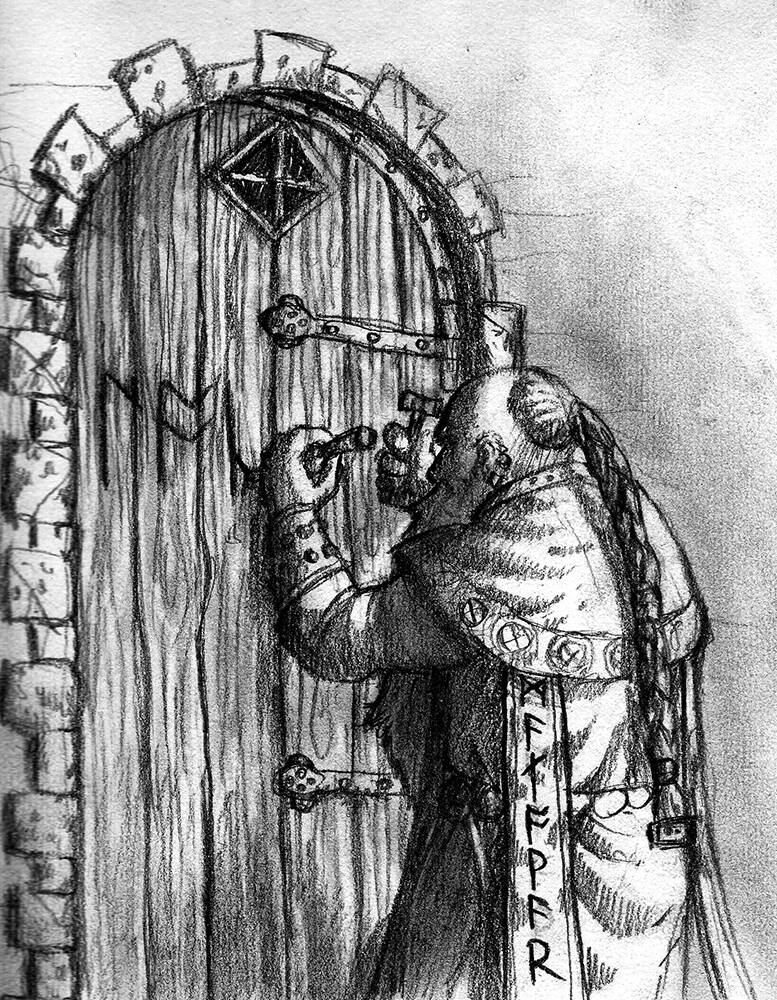
\includegraphics[width=.4\textwidth]{images/Roch_Hercka/dwarvish_runes.jpg}
	\end{wrapfigure}

}{}

\index{Runes}\textbf{Spheres}: Conjuration, Fate, Force, Metamagic, Necromancy

\noindent Dwarves are skilled in the art of summoning magics through carving elaborate runes. Typically they are chiselled, but it is possible to simply `paint a spell' onto a surface.

When spells are summoned, the runes glow -- whether carved or painted -- then giant, ghostly runes can be seen dancing around the source of the spell. Runecrafters summoning illusions might have their illusions appear with a flurry of glowing symbols of trickery -- each sphere of magic and indeed each spell has its own special runes.

Runecasters must devote a single Academics slot to learning how to properly inscribe runes. Their mana stones are always precious metals inscribed with runes such as armour with platinum runes or swords with golden runic inlays. Those mana stones which have an imprinted spell can be activated by either a command word or a condition.

\subsection{Special Considerations}

Runecasters cannot cast spells in the heat of combat -- inscribing runes just takes far too long for Quick Spells. They always use Ritual Spells for the highest level of any Sphere, and can use normal casting after that.

However, in return for this deficite, runecasters can learn their craft far more easily. Each level of a sphere they purchase costs 5 \gls{xp} less than it normally would. While buying Fate 2 would normally cost 10 for the first level and 15 for the second, runecasters merely need to spend 5 \gls{xp} for the first level and 10 for the second. If they ever want to use those same sphere through a different path of magic, they must spend 5 \gls{xp} to `repurchase' each level. For example, someone who could cast both alchemical and runic magic might purchase Conjuration at the second level for a total of 15 \gls{xp}. They could only use it for runic magics, but later they could spend 5 \gls{xp} to be able to cast the first level with either the alchemy path or the runecasting path.

Runes can never be cast in a subtle way. All castings will be entirely obvious. Ritual castings are a particularly long affair, often taking an entire day's work and always require runes to be dented or impressed into something rather than just written out.

\subsection{Mana Stones}

Rune casters mana stones are, of course, runic carvings, and can never be painted onto anything.

\section{The Path of Song}

\label{song}\textbf{Spheres}: Aldaron, Enchantment, Fate, Illusion, Metamagic

\noindent The character has learnt the magic of song. They can sing illusions into existence, inspire people with great tales and enchant people with a lute. Any instrument, song or performance suffices for casting a spell so long as it is appropriate -- a flute is not usually a good way to magically make people scared.

Song spells appear with a flash of colour -- generally on a cinematically appropriate note. They require some noise to activate so they are difficult to hide, but people will not always make the connection between the start of a spell and the strumming of a lyre.

In order to learn the Path of Song, the mage must have the second level of the Performance Skill. 

\subsection{Special Considerations}

Just as with rune magic, song magic can never be cast in an instant.  Quick spells are entirely barred, as a song takes time to be invoked with magic.  And as with rune magic, those on this Path need to spend 5 less \gls{xp} each time they buy a level of some magic sphere.

\subsection{Mana Stones}

The mana stones of the Path of Song are actual songs. The bard composes a song especially for the purpose; when anyone -- anywhere in the world -- plays the song on the correct instrument the mana can be regained. Such songs can also become vessels for spells, becoming magical items which activate once played.

If anyone ever pulls mana from the song (either for a spell casting or because they are low on mana) while the song-spell is empty, it is destroyed forever. The song will be difficult for anyone to remember and will no longer store any mana until someone remakes the spell.

Legends speak of an ancient and secretive group of song-mages composed of bards, dryads and stranger creatures who have spy networks which can transport information far overland to distant areas or even across planes of existence. They swap spell-songs, where one party can constantly check if the song still exists, and when the other party wants to send a message the spell-song is broken to indicate that a mission has begun, or perhaps that someone important is dead and a meeting must be made.

Rare and powerful spell-songs are swapped as currency among bards -- spells which can protect the singer or enchant a crowd.

\chapter{Knacks}\label{knacks}

Characters can individuate themselves by learning various Knacks -- special talents for combat manoeuvres, magic, skills or other abilities. Most people can pick up a couple of knacks but further Knacks become progressively more unintuitive.

\section{Combat Knacks}

\subsection{Adrenaline Surge}

The player can declare that super-human effort is being thrown into an actoin, and gain +1 Strength for that one task.  This can increase damage, but cannot increase Initiative after a \gls{round} has begun.

Adrenaline surge can be used once each scene for each knack the character has, and no more than once a \gls{round}.

\subsubsection{Back to the Wall}

You are particularly difficult to flank. So long as you are not surrounded on all four sides you receive no penalty for being Flanked.

\subsubsection{Brawler}

The character receives +2 to Strike when making unarmed attacks or grappling.

\subsubsection{Charge}
If you spend a \gls{round} moving at your maximum speed in order to engage with the enemy, you can replace your Strength bonus with your Speed Bonus for the purposes of calculating Damage, or add +1 Damage per knack you have, as you prefer, for the first attack of the \gls{round}.

For example, a character with Speed +3 and Strength -1 could charge into the enemy and the first attack would count as having a Strength Bonus of +3 due to the character's momentum being pushed behind that initial sword swing. This Strength Bonus only counts for the purposes of Damage and cannot increase the character's Initiative once combat has begun.

\subsubsection{Cutting Swing}
The character can cut through more than one opponent with a heavy weapon, or slice open multiple skulls with a single arc of metal.  Any time the character reduces an opponent below 1 HP, they can immediately make another attack at no Initiative cost against anyone in range of the weapon; if that attack reduces the opponent below 1 HP then further attacks can be made until no further enemies are within range or the character fails to fell an enemy.

\subsubsection{Disarm}
With a flick of your sword into an opponent's wrist or by trapping the hilt you can throw an opponent's sword away. This manoeuvre takes the normal amount of Initiative for using your weapon. You and your opponent make a Resisted Dexterity + Combat Action, \gls{tn} 7. If the disarm attempt is successful, the weapon is thrown 1D3 squares in a random direction.

\subsubsection{Dodger}
The character is an expert at dodging long-ranged attacks. They need to spend only 1 Initiative point in order to Keep Edgy (see page \pageref{edgy}) and can thereafter dodge all incoming missile attacks with their Speed +2. If this knack is taken multiple times, it adds +1 to the roll each time.

This Knack grants immunity to all Unseen Attacks from Ranged weapons, such as bows or throwing knives, just as long as the user is Keeping Edgy.

This knack is automatically granted by using a medium sized shield, so anyone who both has the Knack and a shield could spend 1 Initiative point at the start of the \gls{round} to be able to dodge all incoming missile attacks. If their Speed were +1, they would gain a +4 bonus to dodging, or anyone attacking them would raise the \gls{tn} to hit this character by 4.

\subsubsection{Expert Flanker}

The character can irritate and distract multiple people at the same time. Each Knack they have allows them to flank an additional opponent and each of those opponents has their Evasion factor lowered by 1 for each Knack the character has. This Knack cancels all effects of the Knack: Back to the Wall for anyone near the character.

\subsubsection{Finishing Blow}

Any attack the character makes of 12 Damage or more gains a number of additional Damage equal to the number of Knacks you have, including Magical attacks.

Purchasing this Knack multiple times only adds +1 to the additional Damage dealt. Many weapons, such as warhammers, come with this Knack in-built, so anyone with the Knack: Finishing Blow, who also wields a warhammer, would trigger +2 Damage any time sie dealt 12 or more Damage, or more if sie had further Knacks. Other Knacks from weapons do not count towards the total.

\subsubsection{First Strike}
The character is well practised at getting the first hit in. They receive +2 Initiative on the first \gls{round} of combat.

This Knack can be taken any number of times, with all secondary uses granting an additional +1 Initiative. For example, while using a spear (which has the Knack: First Strike, in-built), and the Knack, a character would gain +3 Initiative on the first \gls{round} if attacking with the spear.

\subsubsection{Flashing Blades}
The character is an expert with light weapons, i.e. any weapon with a Weight of -2 or less costs 1 less Initiative to wield. Attacking with a dagger would cost 3 Initiative rather than the usual 4.  This Knack cannot be purchased twice.

\subsubsection{Fox Hop}
The character is particularly good at defending themself by jumping about. They receive a bonus to Defence equal to half the number of Knacks they have, rounded up. This bonus does not stack with weapon bonuses.

When using the Aggressive Stance, this bonus goes into the Strike Factor instead of the Evasion Factor, as per usual.

\subsubsection{Furious Blows}
You can wield large weapons exceptionally fast. Medium weapons (those with a Weight Rating of -1 to 4) cost 1 less Initiative to make an attack with just so long as you have no Encumbrance penalty to wielding it. Using this Knack, an attack with a longsword would cost only 5 Initiative. Buying this Knack multiple times has no effect.

\subsubsection{Furious Rage}
You gain +1 to Strike when using the Aggressive Stance.

\subsubsection{Guardian}
The character receives a +2 bonus to their Evasion score for the purposes of defending people and can defend multiple people at once they pay only 1 Initiative for each person they wish to defend. Those people must be close behind them, as usual. When the character is defending themself they use their normal Evasion Bonus.

\subsubsection{Last Stand}
Any time the character loses their last FP they immediately gain +5 Initiative points plus one per Knack the character has. The Initiative Count goes back up to the highest Initiative to let you act (presumably) alone.

Characters also gain a number of \gls{mp} equal to the number of Knacks they have.

\subsubsection{Mighty Draw}
You can draw back a hunting bow in a single \gls{round}, paying only 8 Initiative for the action, minus one per Knack you have. For example, someone with 4 Knacks would pay only 4 Initiative for the attack.

\subsubsection{Perfect Sneak Attack}
Any Sneak Attacks you complete inflict an additional +1 Damage for each Knack you have. Normally, Sneak Attacks inflict +2 Damage, so someone with 3 Knacks would inflict +5 Damage.

\subsubsection{Precise Strike}
You require 1 less to achieve a Vitals Shot. For example, when targeting an opponent with a Evasion score of +2 and Partial armour, they would normally require a score of 9 to hit and a score of 12 to make a Vitals Shot which ignores all armour. With this Knack they still require a score of 9 to hit but only a score of 11 to make a Vitals Shot. People with this Knack can also bypass Perfect armour by rolling 6 points above the target's \gls{tn}.

Multiple purchases of this Knack allow you to bypass armour at an increasingly low \gls{tn}.

\subsubsection{Quick Draw}
You can pull back and shoot a short bow by paying only 3 Initiative. If you have the Knack: Snap Shot, you can pay only 3 additional Initiative to aim.

\subsubsection{Snap Shot}
You pay 0 Initiative to reload an arrow onto your bow, as opposed to the regular Initiative cost of 2. Additionally you can make an Unseen Attack with a bow by paying an additional 4 Initiative instead of spending a \gls{round} aiming.

\subsubsection{Solid Defence}
The character can hold their actions, persistently defending themself rather than attacking. They gain +2 to their Evasion Factor during this time. At any time they can give up the protection just as if they had held their action normally; this allows their to act at 1 higher Initiative than the current Initiative Count.

\subsubsection{Stunning Strike}\label{stunningstrike}
You can declare that you are attempting to stun opponents. You then take a -1 penalty to Strike but if you successfully hit an opponent, all Damage dealt reduces their current Initiative. Multiple uses of this Knack add 1 each to the Initiative loss.

For example, if someone were using a cudgel (which comes with the in-built Knack: Stunning Strike), and also had the Knack, then they smacked someone for 4 Damage, the opponent would immediately lose 5 from their current Initiative Score, even if all of the Damage was mitigated by \gls{dr} and FP.

\subsubsection{Voice of Wrath}
Your battle cries and demeanour are particularly fearsome. Enemies receive a -2 penalty when taking Morale Checks where you are their enemy.

\subsubsection{Ultimate Coward}
You receive a +2 bonus to fleeing from opponents.

\subsubsection{Unstoppable}
The character does not fall incapacitated when falling below 1 HP they makes the usual Vitality Check and if they survive they continue to act until the end of combat, though they also has to take the usual penalty: -1 per Damage beyond 0 HP, in addition to any Fatigue Point penalties. Once combat ends, they fall unconscious. Each time they suffer further Damage a new Vitality Check is made.

Additionally, the character receives a bonus to all Vitality Checks equal to half the number of Knacks they have, rounded up.

Finally, the character gain +1 HP.

\subsubsection{Weapon Shatter}
You are particularly adept at targeting weapons' weakpoints. When using any weapon with a Damage bonus of +2 or greater you can make an attack against an opponent's weapon instead of the opponent. The \gls{tn} is the same as hitting the opponent +2. The attack must cause at least 6 Damage. If successful, blade weapons shatter and count as daggers, giving nothing more than +1 Damage. All other weapons which are successfully destroyed are simply gone, providing no bonuses at all. Certain good quality weapons are immune to this effect.

\section{Spellcasting Knacks}
\subsubsection{Blood Caster}
The caster's magic is fuelled by hatred and tenacity. If the character has 0 FP and loses a single HP then they gain +2 to their effective Intelligence Bonus. If they lose half their HP then they gain an additional bonus equal to the number of Knacks they have. For example, a caster might lose 2 HP then gain an effective +2 bonus to casting Firebolt spells and a +2 bonus to the Damage inflicted by such spells. When they are later struck again and goes down to 1 HP then (since they have 2 Knacks) they gain a +4 bonus to such spells and a +4 bonus to Damage.

This Knack can only be used when there is a legitimate grievance. The mage does not gain the bonus when they have harmed themself. It lasts only until the end of the scene and can reactivate only once the mage has lost further HP.

The Knack might also be used when a member of the party has died, or when someone the character has spent Story Points on has been killed.\footnote{See page \pageref{stories} for Story Points.}

\subsubsection{Combat Casting}
The mage suffers only a -1 penalty rather than the usual -2 when casting a spell using only one hand. Alchemists and divine casters unable to use their voice and hands suffer a -3 penalty rather than the usual -4. Polymorphed creatures still suffer a full -2 penalty to all spell-casting in addition to any other penalties.

\subsubsection{Consume Soul}
The caster can suck the soul from dying humanoids. While something within their normal spell range is dying, they can make a resisted roll against the target where both use their Intelligence Bonuses -- the target receives a penalty for being below 0 HP as usual and the mage receives the normal range penalties for ranged weapons. If the mage is successful they gain back 1 \gls{mp} + the target's Intelligence bonus (to a minimum of 1). This action requires 8 Initiative points and can only be performed when the character is prepared to cast spells that \gls{round}.

This Knack may only be bought at character creation or immediately after the caster is required to take a Vitality Check to avoid death. It may not be taken while following Laiqu\"{e}, Alass\"{e} or V\'{e}r\"{e}.

\subsubsection{Extreme Focus}
The spell caster can focus on a spell to the exclusion of all else. During this time they automatically fail any checks to notice things. All ritual spells cast with this focus grant a bonus to the caster's Intelligence score for the purpose of casting spells equal to half the number of Knacks the character has (rounded up).

\subsubsection{Quick Spell}
The character is particularly adept at casting spells quickly, and therefore in Combat. Spells cost 2 + their level in Initiative, so a 4th level spell would cost 6 rather than the usual 7 Initiative.

\section{Other Knacks}

\subsubsection{Chosen Enemy}
The character has a burning hatred for a particular race of creature. The character gains a -2 penalty when interacting socially with such creatures and a +1 when performing actions such as tracking them, attacking them or intimidating them.

For each Knack the player has, they may select a new chosen enemy, so those with a total of 3 Knacks may select 3 chosen enemies. Those enemies may be chosen at any time, including long after a new Knack as been bought.

Possible enemies include: Forest Creatures, Behemoths, any humanoid race (e.g. Dwarves, Humans, et c.), Nura Beats, Nura Humanoids, Underground Creatures and Undead.

\subsubsection{Fast Healer}
You regenerate unusually fast. Any scene which you end with a rest allows you to heal 2 additional Fatigue Points and 2MP.

\subsubsection{Hardened}
The character is particularly tough and gains +2 HP and immunity to the Knack: Stunning Strike.

\subsubsection{Specialist}
The character specialises in some non-combat Skill, becoming exceptionally good at one particular action. They select a paring of some Attribute + Skill to gain a +2 bonus whenever the two are used. For instance, when using Charisma + Performance to sing a song they could gain the bonus, though when writing one with Intelligence + Performance the Knack would have no effect.

This Knack can be bought any number of times but only once for a particular Attribute + Skill pairing. It can add to rolls to cast spells, but not combat rolls, including ranged combat.

\chapter{Stories}\label{stories}
\index{Stories}Players `write' most of their backstory during play rather than before it. Instead of defining where they come from and what advantages this might bring then using those elements later, during play players have a limited store of `stories' where they retroactively decide upon a piece of the character's history which is currently useful to them. Imagine the players have entered a village -- they really need a weapons smith but that's a rare specialist for a small village. The \gls{gm} informs them there is none, but one player objects. She says `I think I actually know someone in this area' and then spends one Story point from her limited pool of 5. The \gls{gm} decides not to veto the action and the village now has a very competent weapon smith, very willing to help her character out. The character then tells the rest of the party how she and the blacksmith met.

Later the characters are caught in a tight spot in a dangerous town -- the thieves' guild is after them, so one player decides he has a friend in the local temple willing to give them a blessing; this isn't just any friend but a high-ranking priest famous for being able to perform miracles and give potent blessings that will protect anyone from harm. The player spends the requisite points and it is done -- the new priest is created as a character for town.

As sessions roll on, each character in the game inevitably gains a longer backstory until everyone in the group knows exactly where their companions have come from.  Of course, players also have the option of keeping quiet about their history -- playing a mysterious character is really just a matter of holding back the Story Points until the appropriate juncture for a grand opening.

The \gls{gm} is, of course, free to veto any Story suggestions without explanation in order to maintain the integrity of the plot or stop cumbersome play issues. Players begin each with 5 Story points and spend them at any point during the game. The encounters must take place in a rational manner -- players might find the perfect sellsword in a town, but if they're in a dungeon, fighting a hall of ghouls, there's little reason for a random sellsword to be present and looking for a job -- this is not an ability to magically summon useful tradesmen with a flash of smoke and plot. As a result almost all stories will have to be told in populated areas such as towns and villages.

All stories should be noted down on the back of the character sheet, including any stats from companionss, just in case they enter during a later adventure.

\subsection{Downtime}
Story points can be awarded by the \gls{gm} during \gls{downtime} -- generally a short downtime will grant 1 or 2 Story Points while a longer downtime will grant 2 to 3 Story Points.

Some characters may save up their Story Points at this juncture just to buy something expensive later.  Alternatively, characters can use those points to explain what they were doing during the \gls{downtime}.  Perhaps the group earn fabulous wealth and split up for some years, then upon returning one of them has learned dwarvish, while another joined the military and gained friends willing to help out on some new quest.

\section{Sample Stories}

The following is a suggested list of Stories the players can tell and their costs. The players are strongly encouraged to suggest more to the \gls{gm} who will either veto them or give them an appropriate cost.

\story{1}{I know a guy who'd be perfect}
You know someone in town who has just the skills you are all looking for. They might be a farmer, willing to put you and the group up for the night, or someone who knows all the local rumours. If they have some special Skill, such as a weapon smith with a workshop, then they will have a total bonus of +5 to such tasks derived from some combination of Attribute and Skill bonus.

The character in question cannot have any martial or magical Skills.

\story{1}{Perhaps we can make a detour}
You know of a sacred location nearby, perhaps a church, or a shrine or just a sacred cavern where the land is teeming with magic. In this sacred area, anyone stepping into it receives 1 \gls{mp} per \gls{round}. If the spot is guarded by a spirit then this spirit or other creature then sie is friendly to you. The place will not necessarily help you hide or defend yourself unless you are also spending Story points to make it a place to rest.

Those following the Code of Experience gain no \gls{xp} for finding this location.

\story{1}{Oh! Don't I know him}
You recognise a friendly character from some previous Story you have told. The \gls{gm} will explain why they are in town but you are free to offer suggestions. Said characters won't necessarily be as useful as they would be if they were brought into the adventure for the first time with Story points and may only help for a scene, but they should be somehow useful. This may include a trader who was previously known to have valuable information about some situation, or a mage the characters had previously met who could cast a useful spell or two.

\story{1}{I think I heard something about this}
When the \gls{gm} asks you to make a check to gain knowledge, you can spend a Story Point and mention how you know this one particular fact about this topic. You gain a +6 bonus to a single knowledge check. This does not count again for the same domain of expertise -- it is only a bonus to knowing one, single fact about the subject.

A failed roll indicates that while you have a lot of history intertwined with this problem, you are still wrong.

\story{1}{My uncle taught me something about this}
You have a surprising Skill or Knack which will comes in useful. As you tell this story, you can buy a Skill level so long as you have the requisite \gls{xp}. This cannot be a Skill which you have clearly lacked in the past, e.g. if your character has so far been illiterate then you cannot suddenly learn a level of Academics. However, if you have never wanted for Craft ability then you could declare that you have always known how to forge iron, or that you have a Seafaring Skill.

\story{1}{Fun fact about the elvish first person plural}
You have spent a significant amount of time in another culture. You know their language and enough of their background to transfer over basic Skill knowledge. If you have the Performance Skill and are familiar with elvish culture then you also know some Elvish songs. If you are familiar with gnoll culture and have the Empathy Skill then you know a range of details about gnoll etiquette and lineage.

\story{1}{It'll be just like the old days, remember that time}
At the point a new character joins the group you can select one other player and have a shared background with them (or with another, if your character is new). You describe how you previously met and possibly adventured together. From then on, you can split the cost of stories, so if the group wants to find a safe space to rest then instead of one character spending 2 Story points you could each spend 1. Each of you can use characters from the other's background, because all your Stories have the option of being shared stories. If you are both of noble heritage, any money you get must be divided between you. If you are both friends with a skilled armourer, they will only be able to repair one piece of armour at a time.\footnote{This Story is transitive and symmetrical, so if player A shares a background with player B and player B shares a background with player C then player C also shares a background with player A.}

\story{2}{I can talk to a guy who might be interested}
You know a low-down thug, cutthroat, soldier, or sellsword who'd just love to join you for this one adventure for cheap or for a simple favour. They're a typical example of the race with an additional +1 to an Attribute and a +2 Combat bonus or Projectile bonus. Your contact also has 1 Skill at level 2 and one piece of armour, one weapon and one other piece of equipment. Each piece of equipment can be worth no more than 10 \gls{sp}.

For example, your friend might be a human fighter with Strength +2, Speed 0, Dexterity 0, Intelligence 0, Wits -1, Charism 0, with the Skills of Combat +2 and Stealth +2. Their equipment might be Complete leather armour, a poleaxe and rations.

The Story told might be one of once serving in a militia, or on the high seas. Perhaps you are a member of a thieves' guild and know another who'd be willing to help you out. Perhaps you simply have a family member who was once a sellsword.

\story{2}{We'll get a warm welcome here}
The players are in the character's home town or somewhere they're famous. Everyone will receive them well and the character whose town it is should receive any normal information for the area. The character can call upon the aid of up to three specialists as per `I know a guy...', above. If you are a human, you know the local language (an unusual occurrence since almost every human area has its own language).

\story{2}{I know a place we can rest}
You know of a secluded and secret location where you will be safe. Perhaps there is a safe spot in a tavern you know -- a secret room in the basement, or maybe just an abandoned and deep cavern in the hills that nobody knows about.

If your safe space is ever invaded due to events outside your control, you receive both Story points back if it is within the same session or 1 Story point back if it during a later session where the same place is used again.

\story{2}{Fancy seeing you here}
You can add two to the cost of any other Story and tell it at an inappropriate juncture. Your characters might be locked in a dungeon and happen upon a weapon smith in the next cell, with his confiscated weapons lying in a nearby pile outside his cell. They might find a place they can rest in secret inside the terrifying dwarvish city turned into an undead haunting ground. Or perhaps while on the run from bandits they find a helpful soldier hoping to be hired.

\story{3}{Ah! This is near the spot we buried the treasure}
You have access to large funds now that you have returned to this area. Perhaps you and companions, once buried treasure close by. Perhaps a local bank simply has your money, or a rich man owes it to you. The total amount obtained is $2D6 \times 10$ gold pieces.\footnote{Those following the Code of Acquisition gain no XP for gaining gold through Story Points.}

\story{4}{There is a man whom they call}
Your miraculous ally is a mage, or priest or some other \gls{miracleworker}. They will not enter combat with you but will agree to employ whatever magics you wish. Their Attributes will be each 0 plus the racial modifiers, except for Intelligence, which will always be +2 precisely. They will have 1 Skill at level 2 and another at level 1. Their Mana points will be 6 in total, after the Intelligence modifier. One magical sphere will be at level 4, another at 2 and another at 1. This mage walks only a single Path of magic.

\story{4}{My boys should still be around here}
You know some militia, famous for fighting together. You might remember your old war buddies who'd come out on any mission for you, or know of a rag-tag bunch of horrible cut-throats who'd be willing to do any job for a \gls{sp} and a dram. The total number of people available is equal to 3 + your Charisma Bonus.

The Traits of each fighter are identical to those in the `I can talk to a guy who might be interested {\dots}'.

\story{5}{Do you know who I am!?  Because I happen to be}
You are the child of minor nobility -- perhaps a knight errant or son of a Town Master. You can collect $2D6 \times 5$ gold pieces from your homeland -- and if you pass a Charisma + Empathy task (\gls{tn} 10) you can double it due to asking your parents extra kindly. If, on the other hand, the money is yours then you can start with it by taking this Story when you begin play but cannot ever double your money by asking parents for more. You have access to a minor keep -- either your own or a parent's -- and can demand the services of any skilled tradesman in the land except for magical talents. You do not have special military access but can buy their swords for the usual rate.

\story{7}{My father will give us a royal welcome when we get to}
You are revealed to be the child of royalty or some other type of nobility, and you are returning to your kingdom. You can request almost anything from the royal family, within reason, including $3D6 \times 10$ gold pieces (double with a successful Charisma + Empathy task, \gls{tn} 8). While with your family, you can use up to 6 story points each adventure. With these you can purchase men at arms, demand the help of tradesmen or any other story except for learning a language.

Since this Story costs 7 Story points, no player should expect to use it until there has been some downtime -- if the character starts out claiming to be a prince then it will be a long time before the story recognises this claim.

\section{Combining Stories}

Whether telling one story each adventure or letting everyone know all about your character's backstory all at once, players are encouraged to think about weaving their stories together. You may have told us that you learnt gnomish when staying with the gnomes. Now that you need a blacksmith in this village, why not specify that he's a gnome whom you once knew? \ And if you need a sellsword to join your group later, how about specifying that you once fought with him to defend the gnomes?

Alternatively, if you are taking out all your stories at once, you might want to declare that you know a mage who lives in a place you can access through a nearby secret portal. You instantly adopt a safe space and a helpful magical ally, then start expounding upon the days when the alchemist was proudly telling you about his impregnable home.

\iftoggle{verbose}{
\section{The Call to Adventure}
Groups of adventurers form for any number of reasons, and your \gls{gm} may already have a solid plan in place.  However, let's jump through a few ideas just in case you need a hand gettings started.

\subsection{The Night Guard}
Fenestra doesn't have many wars or diseases, but it never becomes overpopulated.  The reason is simple: monsters.  There are giant arachnids in the forests, bassilisks which belch poison and steal cattle, and the occasional dragon.  If someone can't find a useful way to employ themselves, someone's waiting for them to join the Night Guard.

The majority if the night guard have the dangerous, boring, and thankless jobs such as guarding cattle, patrolling for nura, and occasionally clearing an area where suspected monsters guard territory.  A few go onto more dangerous jobs such as hunting nura, tracking down criminal gangs, or espionage.

Some rare few have been known to strike deals with dragons to leave an area, or assassinate rogue alchemists who are powerful enough to keep themselves free from the reaches of any magical guild.

In general, the more dangerous the job, the higher the pay, so most of the Night Guard try not to do too well at their job.  They train in archery well, take a paycut in return for having more members in their group, and make sure nobody volunteers them for anything interesting.  Of course, a lot of the jobs one takes depends more upon a captain of the Guard than the grunts.

\subsection{Defending the Fatherland}
Your homeland is in grave danger as nura surround it and grow more numerous every day.  The local lord has given you strict instructions that you cannot leave, but you feel sure that the only path is to get help from another group.

Once each member of the group has expended three Story Points, an oppening comes to travel to a nearby ally, and beg for an army to save your homeland.

The characters may all be gnomes, defending against encroaching nura who have come through a portal, while the elders constantly argue that if only \emph{somehow} someone could get down there and destroy the portal, everyone would be safe.  But that ``somehow'' never comes, and the monsters are coming up faster and faster.  Rumours abound of distant elves who might help, but they have their own problems.

Alternatively, the party may be elves, constantly assaulted by increasing undead assaults, spurned on by an increasingly powerful and paranoid necromancer.  Nobody wants to contact the local dwarves to ask a favour, but once the greatest of the local bards die, everyone knows that the party is over.

\subsection{The Magical Guild}
The characters are all alchemists in the service of the Alchemist's Guild.  The first part of the campaign involves high-school rivalries against other Clans in the guild such as stealing their homework, or vying for romantic attention.  Soon after, the characters begin proper guild missions, venturing out into the strange areas of the world where normal people will not tread.

\vspace{.2cm}
\begin{tcolorbox}[arc=1mm,tabularx={llp{.5\textwidth}}]
	Clan Alisa & Force & Stonemasons who eventually rose to magic workers. \\
	Clan Kisha & Conjuration & The priesthood of Laiqu\"{e} who abandoned their god to study alchemy. \\
	Clan Stein & Invocation & A military clan who maintain ties with the College Outpost at the Coast. \\
	Clan Ventress & Illusion & An old family who lived in Eastlake since before the College. \\
\end{tcolorbox}
}{}

\vspace{.2cm}

\iftoggle{verbose}{

	\hrulefill

	{\itshape ``Do you think the village on the other side of the mountain is safe to visit?'', asked Thenton with raised eyebrows.

His companions did not really want to hear that question, but they had.  It was impossible to tell from this distance if the nura had settled there already.

``Ah dinnae ken, laddie''

Hugi is resolved to just enter the next area, stoically, but his player is no stoic. It is decided that now is the time to expand Hugi's backstory. He wants a place to rest, he wants more of an idea of what is happening here. He decides to spend a Story point to specify that a single dwarven outpost has a single person still there.

``Why is just one person in an outpost?'', the \gls{gm} asks.

``Well, it's my cousin. She was inside at the time. When the scouts returned from watching the side of the mountain, they all got eaten by nura. Only after that she managed to escape, helped by the men-dwarves. So she's alone in the outpost''

``So this is a safe space story?'', the \gls{gm} asks.

``No. No I just want to spend one Story point and get someone with a normal place to stay, and knows a little about what's going on, and maybe some knowledge of Medicine''.

Hugi's player marks off a single Story Point and starts telling his story.

``There's an outpost over there'', Hugi remarked. ``It looks mostly like the mountain but you can see a little dark bit that's too straight-cut. They're little windows.''\newline

Entering the building, Hugi found his cousin, Magda. Thenton expected them to hug after the ordeal, but Hugi just bowed low. Apparently he was proud of the honour of gathering news from her on account of their shared blood.

As luck would have it, she was a proficient medic, and helped patch Hugi back up, safely removing the arrow. Her story was unexpected though.

``They didnae come up from caverns below but fae above. We didnae un'erstan' at first, but it was in the music. As new hobgoblins took up arms, they wouldnae all attack, but only sing. There's evil in them songs, and the dwarves all around started the painful transformation into nura. They didnae immediately change, but the other dwarves couldnae be held back and they started in at the newly changed companions, hacking them apart. With their mind rattled an' fearin' fer their skins, they started attackin' back, and the original hobgoblins behind them at least new not tae provoke.

``It wasnae long afore everyone was changin' an' nothin' could be done. Some brave ones helped the wimen awa' fae the depths with a side-tunnel. The rest were got, but ah got oot alaen. I dinae think thar's anyone doon thar any more.''
}}{}

\clearpage\chapter[Gods \& Codes]{Gods \& Codes}
\label{gods_codes}\index{Gods}\index{Codes}Players can receive small amounts of additional \gls{xp} for following their beliefs. While anyone is free to give offerings to any of the gods, most people have a primary god they worship, suggested by their birth but decided in adulthood based on shared values. Others follow no god but have a code of some type, guiding their actions. These codes are not formal beliefs, written as law and discussed at meetings but rather a set of aspirations which some have.

The \gls{gm} decides how much \gls{xp} to give out for any given task -- each path has a number of suggestions but the list should be understood as open-ended and entirely at the whim of the \gls{gm}.

Some codes give a reward for donating or gaining gold.  Only the highest reward counts, so someone cannot gain 1\gls{xp} for donating a gold piece to a temple, and then gain 10 more for donating 100GP -- the highest sum takes precedence.

\section{Gods}
Each god has a holy day marking its favourite time of year. During the holy day, anyone can earn \gls{xp} by following the edicts of the god, even those who follow others. The day of Ohta is a day to remember war and settle disputes by fist or steel, the day of Alass\"{e} is one of joy, to be celebrated with pranks and presents.

The gods are most popular with humans and gnolls. Most dwarven settlements have a temple of some kind but it is not something all dwarves take much interest in except during odd times when they want to pay for a blessing. Gnomes' interactions with the gods mainly consists in chronicling legends about them and debating the nature of divinity, but not actively worshipping them. Elves, it is said, do not have the humility to worship anything.

The gods presented here are the most important -- they are the ones featured in the larger tales and who have the most prominent holy days. There are, however, many more. Each region or individual tribe has its own little god. Players are encouraged to create their own.

The calendar of Fenestra is a strange one. The four seasons are different from ours and they change each year -- some years have cold seasons, others have stormy seasons where volcanoes explode and lightning is a regular occurrence. There are three different types of these four-season `cycles', then the calendar repeats.

\subsection[Alass\"{e} -- Goddess of Joy]{Alass\"{e} -- Goddess of Joy}
\index{Gods!Alass\"{e}}(`alAS-seh')
The goddess of joy delights in pranks and fun of all kinds. Her holy day is in the third season of the first cycle -- a cold time when people are in need of cheering up from the cold winds, when her followers stuff snow down people's back or balance ice-plates on the tops of doors to watch them fall on friends' heads. An eclipse marks the actual day every three cycles.

Her temples are always full of home-brewed beer served by attractive men and women. Often such temples replace regular taverns.

\begin{xpchart}{Alass\"{e}}

	1 & Playing a prank \\

	1 & Donating at least 1 gp to the church. \\

	1 & Drinking and eating to excess. \\

	1 & Giving food or shelter to the needy. \\

	3 & Winning a drinking competition. \\

	3 & Lifting the spirits of the downtrodden. \\

	3 & Creating a funny song. Requires at least a full night and an Intelligence + Performance action, \gls{tn} 10. \\

	3 & Playing a prank set up last session. \\

	5 & Hosting a feast for a village. \\

	5 & Creating a new type of alcohol. \\

	5 & Saving someone's life. \\

	10 & Playing a prank set up two sessions ago. \\

	10 & Saving a village or larger populated area from destruction. \\

		\end{xpchart}

Priests of Alass\"{e} have access to the illusion and polymorph spheres. Their spells appear with a flash of rainbow colours, often accompanied by light, strange sounds similar to a harpsichord. Their mana stones can be anything which is a simulacrum of anything else -- a toy dagger, a doll, a statue or a painting are all possible mana stones. Their mana stone spells are activated by a command word.

\subsection[C\'{a}l\"{e}]{C\'{a}l\"{e} -- God of Illumination}\index{Gods!C\'{a}l\"{e}}(`Kaah-leh')

The god of light is popular among all the land, especially with scholars, as he is a god of knowledge. His holy day is during a warm season -- the first part of the second cycle -- when the most light shines on all the world. During this day, a great black eye can be seen travelling across the Ainumar -- the nearby celestial orb where it is said the gods live. His followers are devoted to uncovering secrets and preserving all knowledge. His temples often take the form of libraries and his services are often readings of important books from non-religious sources as well as holy works concerning other gods.

Followers of the god of light have access to the illusion and force spheres. His mana stones always contain the writings of famous works -- usually from the Holy Book of Light but potentially from any learned source. The item in question must be at least as large as a sheet of paper -- commonly a book, potentially an armoured breast-plate but never a sword or rock. His spells appear in a warm glow of light, illuminating an area with a glow the strength of a few candles brighter than the ambient lighting. The mana stones of C\'{a}l\"{e} are always activated by a command word.

\begin{xpchart}{C\'{a}l\"{e}}
	1 & Donating at least 1 gp to the temple. \\

	1 & Learning a new secret. \\

	1 & Gaining a new level in Academics or any sphere in the Path of Alchemy. \\

	1 & Crafting a new magical item. \\

	1 & Overcoming a tricky situation. \\

	3 & Solving a complicated puzzle. \\

	5 & Donating at least 10 gp to the temple. \\

	5 & Uncovering a conspiracy. \\

	10 & Solving a legendary puzzle. \\

	10 & Donating at least 100 gp to the temple. \\

	10 & Writing an informative book on some topic. Intelligence + Academics is rolled at \gls{tn} 12 during downtime. \\

	10 & Converting someone to the god. \\

	15 & Finding and preserving important knowledge that would otherwise have been destroyed forever. \\

\end{xpchart}


\index{Gods!Laiqu\"{e}}\subsection[Laiqu\"{e} -- Goddess of the Forest]{Laiqu\"{e} -- Goddess of the Forest}(`Lie-queh')

	\begin{xpchart}{Laiqu\"{e}}

	1 & Donating at least 1 gp to the temple. \\

	1 & Finishing a battle with 0 FP. \\

		1 & Hunting one's own food and dedicating it to Laiqu\"{e}. \\

	1 & Gaining a new level in the Survival Skill. \\

		3 & Building a shrine -- requires 3 days work and an Intelligence + Crafts action, \gls{tn} 8. \\

	3 & Donating all of one's money to the temple. \\

	3 & Freeing a creature from captivity. \\

	3 & Destroying an `unnatural' creature such as an undead thing or a nura which has wandered above-ground. \\

	5 & Finding a new type of creature. \\

		10 & Composing a song to Laiqu\"{e} -- requires an Intelligence + Performance action, \gls{tn} 10. \\

	10 & Converting someone to the god. \\

	10 & Establishing a new temple. \\

	15 & Saving some miles of land from being despoiled. \\

\end{xpchart}

Laiqu\"{e} is the mother of all the growing green plants and all the animals. Farmers worship her as they know their products ultimately stem from the forest and her holy day is a feast-day during the warm first season of the third cycle. She has few temples but many followers. Those temples are usually arranged around some particularly striking tree, often magically altered to appear fantastically beautiful or just warped. Farmers are fond of putting up a little shrine to her with no more than a few rocks and a unique tree, and sometimes with a bird feeder. Her followers are numerous -- they meet during feast days, especially Laiqu\"{e}'s own day of feasting. On other days, they simply travel, and expect Laiqu\"{e}'s blessings and the good will of the people around them to provide food for them, occasionally giving out her blessings if they have been initiated into the secrets of her divine powers.

Those casting spells on her Path of Divinity find things appearing in a wave of mist while flowers bloom nearby. They are granted access to the polymorph and conjuration spheres. The mana stones of her followers are always animals or plants. If the animal in question has access to a spell, the animal as well as the priest always has the ability to cast spells. Her followers commonly have large dog companions which are able to give blessings or summon other dogs for help with the conjuration sphere. Plants with a spell are always activated by a command word. Animals with a spell implanted always activate the spell at their own behest and rarely at the right time; cats have been known to use implanted spells to hunt prey while a dog which feels threatened might reflexively summon aid with a conjuration spell.

\subsection[Ohta -- Goddess of Battle]{Ohta -- Goddess of Battle}
\index{Gods!Ohta}(`och-tah', with a `ch' as in `loch')

Qualm\"{e}'s big sister, Ohta, is a mighty warrior. To be worthy of her, people must train well and be fast in battle. Her temples are few and are often no more than small rooms within a larger barracks, but her priests travel on almost every martial campaign -- even those who follow other gods usually object to going into battle without the blessings of a cleric of Ohta.

Ohta's feast day ends the fourth and last season of the third and last cycle. On this day, if no battles are present, entire towns sometimes gather together to voice their frustrations, calling each other out to one-on-one fights. There is no reprisal for the result of these fights -- they stand alone, and no redress can be made in a socially acceptable way until Ohta's next holy day, three cycles later.

\begin{xpchart}{Ohta}

	1 & Donating at least 1 gp to the temple. \\

	1 & Finding an interesting battle trophy. \\

	1 & Gaining a new level of the Combat Skill. \\

	1 & Surviving a skirmish while outnumbered. \\

	1 & Going first in the party when entering a dangerous situation. \\

	3 & Answering a one on one challenge. \\

	3 & Killing three opponents single handedly in one battle. \\

	3 & Killing a more dangerous opponent than ever before (danger is measured in \gls{xp}). \\

	3 & Surviving a large scale battle while outnumbered. \\

	5 & Donating at least 10 gp to the temple. \\

	5 & Killing five or more opponents single handedly in battle. \\

	5 & Killing a dangerous opponent (16+ \gls{xp}) single handedly. \\

	10 & Killing a dangerous opponent (10+ \gls{xp}) without wearing armour (either mundane or magical). \\

	10 & Donating at least 100 gp to the temple. \\

	10 & Defeating a previously victorious opponent. \\

	15 & Starting a war. \\

\end{xpchart}

Clerics of Ohta have access to the invocation and conjuration spheres. They enjoy summoning weapons, hordes of helpers and raining down divine wrath in the form of fire and lightning upon their opponents. Their spells are accompanied by loud, terrifying noises which can be heard for up to a mile around and shining, silvery flashes from where fire, wild dogs, bears or attacking swarms of bats might appear. Their mana stones are weapons, armour or hunting trophies. Weapons can only store 2 MP per point of Damage they inflict and spells in these mana stones are always activated by a condition. Armour is the same but can only ever store 2 MP. Hunting trophies can hold up to 1 MP per HP of the beast killed.

\subsection[Qualm\"{e} -- God of the Grave]{Qualm\"{e} -- God of the Grave}
\index{Gods!Qualm\"{e}}(`Qual-meh')

Ohta's less popular little brother rules over death and the suffering which precedes it. He teaches us to remember our own dead fondly and to desecrate the graves of our enemies so that they can be forgotten. His feast day is during the great storms of the first season of the first cycle. Volcanoes often explode to mark this occasion. His temples are few and far between -- a couple of large cities with important people buried, the occasional gnoll hut where a mad shaman of death collects skulls and speaks strange promises about a coming war or a deep, dwarven catacomb where the honoured dead of many a dwarf want to gain the promise of being lead to the halls of the honoured dead.

\begin{xpchart}{Qualm\"{e}}

	1 & Donating at least 1 gp to the temple. \\

	1 & Desecrating the bodies of an enemy. \\

	1 & Gaining a new level in the necromancy sphere. \\

	1 & Giving someone blessings upon their death bed. \\

	3 & Performing an outlandish burriel, with sacrifices and words appropriate for the deceased. \\

	3 & Erecting a shrine to the dead. Requires an Int + Craft action, \gls{tn} 9, at at least 10 gp. \\

	3 & Summoning the spirit of a famous person. \\

	3 & Gaining a large body-part from a famous person, now deceased. \\

	5 & Donating at least 10 gp to the temple. \\

	5 & Falling below 0 HP. \\

	10 & Building or funding a mausoleum. Takes a year and requires at least 100 gp. \\

	10 & Converting someone to the god. \\

	10 & Falling below -3 HP. \\

	15 & Falling below -5 HP \\
\end{xpchart}

Clerics of Qualm\"{e} have access to the necromancy and invocation spheres. Many burn their enemies to death and then raise the blackened corpses from the grave. Their spells arise in a pool of inky blackness and are accompanied by the foul smell of old, rotting meat. Their mana stones are always made from the glorious dead.  Mana stone can hold half the FP of the original target (rounded down).  The hand of a man who had 6 FP could store up to 3 MP.  \gls{xp} can also be used as a basis for establishing a glorious target -- any significant chunk of a corpse can hold one third of its \gls{xp} cost in mana, so a dragon worth 22 \gls{xp} could hold up to 7 MP.

Spells implanted in those mana stones are always activated by a command word.

\subsection[V\'{e}re -- God of Justice]{V\'{e}re -- God of Justice}
\index{Gods!V\'{e}re}(`vEH-reh')

Warden to all oaths, lord of a hundred holy warriors, leader of armies, the giver of vengeance and punishments -- V�re is a popular god. He is invoked during wedding vows and business deals. His followers are found among the politically influential and can be some of the most zealous of religious followers. He values obeying the law, making fair deals, being a good host and supporting the poor.

His holy day is during the second season of the second cycle. It is considered extremely good faith to make an oath on this day, and mortally bad luck to break such an oath.

Followers of V�re who break any deal cannot gain \gls{xp} until they atone for the crime.

\begin{xpchart}{V\'{e}re}

	1 & Donating at least 1 gp to the temple. \\

	1 & Enforcing a law. \\

	1 & Feeding the poor. \\

	1 & Hosting guests. \\

	1 & Punishing law breakers. \\

	1 & Returning someone's valuables to them. \\

	3 & Enforcing a major law or imposing the law on a group. \\

	3 & Donating at least 10 gp to the temple. \\

	3 & Making an oath to begin upon a major quest. \\

	5 & Creating a peace treaty between factions in danger of fighting. \\

	5 & Creating a peace treaty between warring factions. \\

	10 & Donating at least 100 gp to the temple. \\

	10 & Converting someone to the god. \\

	15 & Deposing a tyrant. \\

\end{xpchart}

V�re's clerics can access the enchantment and force spheres. They use enchantment to gain followers, dazzling them with the glory of the purity and strength of their god while force is used to protect the innocent and faithful. Their spells appear in a shimmer of gold. V�re's mana stones are always people who are followers of V�re. Those believers alone can activate any spells which are stored inside them. Priests of V�re often gift their followers with single-use magical powers, such as the ability to call upon a blessing or the ability to protect themselves with armour. If the people who are being used as mana stones are given spells then they can activate those spells at will with a short prayer at an Initiative cost of 8.

\section{Codes}
\index{Codes}Those without a dedicated deity often dedicate themselves to some informal code instead. The codes might be thought of as attitudes or philosophies for life. Followers of similar codes may well get along together but they will not recognise each other as members of a similar organisation. Those with a code as their primary motivator may also sacrifice to gods or even occasionally worship and donate to temples, but their ultimate aims lie with themselves. It is said those who do not fully dedicate themselves to any god must wander the afterlife without aid or guidance -- such spirits always provide the most bizarre and contradictory accounts of death and can prove difficult to summon.

\subsection{The Code of Acquisition}\index{Acquisition, Code}
The goal of life is acquisition. We all want things, therefore people who get more things are doing better. Those on the code of acquisition are often those who can acquire more money -- townmaster, dwarves in love with gold or gnomes who have dedicated their lives to finding the best rubies.

Those following the Code of Acquisition who lose their gold cannot earn \gls{xp} for gaining wealth until a similar amount has been regained.

\begin{xpchart}{the Code of Acquisition}

	1 & Buying an expensive item -- worth 1 gp or more. \\

	1 & Being greeted deferentially by a stranger. \\

	1 & Finding out you are the richest person in a settlement. \\

	3 & Buying a very expensive item -- at least 10 gp in value. \\

	3 & Acquiring new currency -- at least 10\% of the current total in value. \\

	3 & Hiring a new servant. \\

	5 & Acquiring a lot of new gold -- at least 50\% of the current total. \\

	5 & Starting a successful new business. \\

	5 & Gaining a new title such as a guild master or townmaster. \\

	5 & Buying an extremely expensive item -- at least 50 gp in value. \\

	10 & Marrying into a prestigious family. \\

	10 & Acquiring a horde of new wealth -- at least 100\% of the character's current total. \\

	10 & Buying an expensive new home -- at least 200 gp in value. \\

	15 & Acquiring grand, new riches -- at least 200\% of the character's current total and at least 100gp. \\

\end{xpchart}

\subsection{The Code of the Tribe}\index{Tribe, Code}
What's important is you and yours. Your children, the memory of your grandparents, the honour of the tribe. Your children will be your legacy, while you must die your legacy can live on forever. If you want to do well in this world, you have to put you and yours first. This path is popular among gnolls, humans and dwarves, who can become very family-focussed. Exactly who counts as being `in the tribe' does not have to be limited to blood relatives, however -- it's an intuitive thing. You know your own.

Travelling companions do not automatically count as members of your tribe, but they may come to in time. Exactly what counts as a `tribe' is mostly in the hands of a player, though the bonds should never be made lightly.

\begin{xpchart}{the Code of the Tribe}

	1 & Helping out a member of the tribe. \\

	1 & Greeting a member of the tribe during a long time away. \\

	1 & Welcoming a friend into the tribe. \\

	1 & Testing a potential new member of the tribe. \\

	1 & Defending your tribe's honour. \\

	3 & Spreading the honourable name of the tribe to outsiders. \\

	3 & Entering battle simply for the sake of the tribe. \\

	5 & Forming an alliance for the tribe. \\

	5 & Returning home after an extended trip away. \\

	5 & Acquiring a new home for your family. \\

	5 & Saving a member of the tribe from some terrible situation. \\

	10 & Fulfilling the final wishes of an ancestor. The ancestor's wish can be specified only while spending Story points on something else and must later be accomplished. \\

	15 & Starting a family. \\
\end{xpchart}

\subsection{The Code of Experience}\index{Experience, Code}
The world is here to be lived, to be known, to be connected with. You want all the experiences -- unique experiences, sacred experiences, horrible experiences; it's all good. You want to stare at the full moon while drinking with friends, to create some new piece of art and to feel enough heart-ache to make you physically sick. Elation and deep-rooted fear are equally valuable -- they are both life. You also value giving life and meaning to the old and abandoned, to experiencing what few others have experienced, whether it's finding a lost and neglected poem from an old language or visiting an area never before seen by people.

\begin{xpchart}{the Code of Experience}

	1 & Finding a new type of food or drink. \\

	1 & Witnessing a flower open. \\

	1 & Taking HP Damage for the first time. \\

	1 & Learning a new type of instrument or any creative specialisation. \\

	3 & Learning a Skill or sphere to a level above any other Skill or sphere you have. \\

	3 & Finding a new friend. \\

	3 & Experiencing any emotion to heights never reached before. \\

	3 & Returning home after a long time away. \\

	3 & Finding a mana lake. \\

	5 & Experiencing deep tragedy. \\

	5 & Falling in love. \\

	5 & Creating a masterpiece of some kind at \gls{tn} 12. Each type of thing can only be attempted once to gain this \gls{xp}. \\

	5 & Discovering a lost piece of art or literature. \\

	10 & Finding an area lost to all contact for more than a century. \\

	15 & Finding an area never before visited by people. \\

\end{xpchart}

\iftoggle{verbose}{
\hrulefill
\begin{wrapfigure}{O}{.4\textwidth}
\includegraphics[width=.4\textwidth]{images/Boris_Pecikozic/dwarves_meet.jpg}
\end{wrapfigure}

{\itshape While all the players are thinking about the next move, the \gls{gm} adds up their \gls{xp}. They defeated 6 hobgoblins and 1 ogre. Hobgoblins and ogres are worth 7 each. There were seven in total, so that means 49 \gls{xp} in total, minus one \gls{xp} per member of the group. The final result is that each character receives 15 \gls{xp} and one more \gls{xp} is left in the pot for later (because 46 cannot evenly be divided by 3). After that, each player wants a little additional \gls{xp} for following their own God or codes.

Arneson follows the Goddess, Laiqu\"{e}. He receives 3 additional \gls{xp} because the nura are particularly hated enemies for him - followers of Laiqu\"{e} believe they are either unnatural, or that their presence in the human realm is unnatural. Hugi, meanwhile, follows the Code of the Tribe; what's important to him is his dwarvish clan's honour. In coming here he has defended his tribe's honour and claims 3 \gls{xp} for coming to the rescue of dwarves in the name of his own tribe. He is additionally helping a particular member of the tribe whom he has met a long way from home. That's another 2 \gls{xp}. He believes his arrival has saved this cousin. The \gls{gm} thinks this is plausible, since his cousin Magda was previously stranded with little food. This grants him another 5 \gls{xp}. Finally, he has spent a Story Point this scene, so he expands that story with Magda, stating that his grandmother came from these mountains, and it was her dearest wish that her grandchildren someday visit that land and see the grand cities where she grew up. Hugi is close enough to the citadel to have fulfilled her dying wish and gains 10 more \gls{xp}. That's a total of 20 \gls{xp}.

Hugi's total of 35 \gls{xp}, he decides to purchase the Knack `Chosen Enemy (Nura)'; it's his first Knack so it costs 5 \gls{xp}. A further 10 \gls{xp} boosts his Base MP from 2 to 4. 10 more boost Base FP from 5 to 10. Lastly, he purchases the Combat Skill at +1.

Meanwhile, Arneson purchases Dexterity +1 with his 15 \gls{xp}. The group is a little older and wiser, and are more confident about meeting danger in the future.

Hugi was filled with pride to the point of forgetting about the pain when Magda pulled out the arrow which had so deeply penetrated his shoulder. He was almost caught smiling when Magda bandaged up the ogre's teeth-marks on his face - it would make a good scar.

The band took only a couple of hours before they set off again, hoping to find that village, somewhere beyond the mist. What had happened to that bard, they could only guess, but there seemed little chance of finding him in that village.

}
}{}

\appendix

\titleformat{\chapter}[display]
{\bfseries}
{
\begin{tikzpicture}
\node[minimum width=\textwidth, text=black!25, fill=black!25, inner sep=1, outer sep=0, anchor=south] (rectinit) {\huge CHAPTER};
\node[minimum width=.8\textwidth, text=white, inner sep=1, outer sep=0, anchor=south west, text width=.8\textwidth, align=right] at (rectinit.south west) (chapname) {\huge APPENDIX~~};
\node[minimum width=.2\textwidth, inner sep=0, outer sep=0, anchor=south west, text width=.2\textwidth, align=left] at (chapname.south east) {\chapnumfont\textcolor{chapnumcol}{\thechapter}};
\end{tikzpicture}}
{0pt}
{\Huge}

\addappheadtotoc

\chapter{Character Creation}\label{charactercreation}\index{Character Creation}

Okay, so you know how to make a character by now.  But just for reference, let's get some procedure down:

\begin{enumerate}
	\item{Roll the dice to determine your race and attributes.  Page \pageref {character_rolls}.}
	\item{Spend 50 \gls{xp} on Attributes, Skills, MP, Knacks, et c, with the Trait charts below, taking $n$ as the current level of of the Trait (or the number of Knacks, or the level of \gls{fp}). Page \pageref{xp}.}
	\item{Take 2 items worth 10sp or less, plus 1 item per Skill level your character has.  Page \pageref{goods}.}
	\item{Select a God or Code to follow, so you can gain \gls{xp}.  Page \pageref{gods_codes}.}
	\item{Starting money is $(3D6-5)^A \times 2^S$cp, where A = levels in Academics and S = combined levels in all specialist Skills.}
	\item{Start the game.}
%	\item{Spend Story Points any time you can.}
\end{enumerate}

\begin{multicols}{2}
\begin{xpbox}{B}
	Result & Attribute Bonus \\\hline

	2 & -3 \\

	3 & -2 \\

	4-5 & -1 \\

	6-8 & 0 \\

	9-10 & +1 \\

	11 & +2 \\

	12 & +3 \\

	\end{xpbox}

\begin{xpbox}{B}
	Trait & Cost \\\hline
	Attributes & $5 \times 2^n + 10$ \\
	Skills & $5 \times (n + 1)$ \\
	Combat/ Projectiles & $10 \times 2^n$ \\
	FP Base & $5 \times 2^n + 5$ \\
	MP Base & $5\times 2^n$ \\
	Magic Sphere & $5 \times 2^n + 5$ \\
	Knack & $5 \times (n + 1)$ \\
\end{xpbox}

\end{multicols}

	\begin{tcolorbox}[arc=1mm,tabularx={lll}]

	Roll & Race & Adjustments \\\hline

	2-3 & Gnoll & +1 Strength, +1 Speed, -1 Intelligence, -1 Charisma -2 \\

	4-5 & Dwarf & +1 Dexterity, -1 Speed \\

	6-8 & Human & +1 Strength, -1 Wits \\

	9-10 & Elf & +1 Wits, -1 Strength \\

	11-12 & Gnome & +1 Intelligence, +1 Dexterity, Strength -2, Speed -1 \\

\end{tcolorbox}

\chapter{Combat}

\begin{multicols}{2}

\initiativechart

\columnbreak

\armourchart

\moralechart

\end{multicols}

\pagebreak

\weaponschart

\pagebreak

\printglossary

\printindex

\pagestyle{empty}

\begin{tcbposter}[
  coverage = {
      spread,
      %interior style={bottom color=white},
      watermark text={BIND},
      watermark color=black!25!white,
      watermark opacity=0.4
  },
  poster   = {showframe=false,columns=11,rows=12},
  boxes    = {
      enhanced standard jigsaw,sharp corners=downhill,arc=7mm,boxrule=.6mm,
      colback=white,opacityback=0.7,colframe=black,
      title style={left color=black,right color=white},
      fonttitle=\bfseries
   }
]

%----
% try removing 'interior engine'
\posterbox[blankest,interior engine=path, halign=center,valign=center,colupper=white!25!black,
	]{name=title,column=1,span=11,below=top}{
		\vspace{.3cm}
		\begin{tabular}{llllll}
			Name: & \vlongline & Player: & \vlongline & Code: & \vlongline \\
			\\
			Concept: & \vlongline & Race: & \vlongline & Culture: & \vlongline \\
		\end{tabular}
		\vspace{0.3cm}
}

%----
	\posterbox[adjusted title=Attributes]{name=attributes,column=1,row=2,span=4,rowspan=2}{\vspace{-.3cm}\begin{tabular}{ll}
		& {\tiny Penalties \hspace{1cm} Bonuses} \\
		Strength & \attributecircles \\
		Dexterity & \attributecircles \\
		Speed & \attributecircles \\
		Intelligence & \attributecircles \\
		Wits & \attributecircles \\
		Charisma & \attributecircles \\
	\end{tabular}}
%----

	\posterbox{name=gumption,column=5,row=2,span=3,rowspan=2}{

	\vspace{.2cm} {\small HP}

	\begin{tabular}{p{0em}p{0em}p{0em}p{0em}p{0em}p{0em}p{0em}p{0em}p{0em}p{0em}}

		\ding{108} & \ding{109} & \ding{109} & \ding{109} & \ding{109} & \ding{109} & \ding{109} & \ding{109} & \ding{109} & \ding{109}  \\
		\tenboxes
	\end{tabular}

	\vspace{.6cm} {\tiny Fatigue}

	\begin{tabular}{p{0em}p{0em}p{0em}p{0em}p{0em}p{0em}p{0em}p{0em}p{0em}p{0em}}

	\tenboxes
		\ding{111} & \ding{111} & \ding{111} & \ding{111} & \ding{111} \\
		\ding{182} & \ding{183} & \ding{184} & \ding{185} & \ding{186} & \\
	\end{tabular}

	}
%----
	\posterbox{name=mp,column=8,row=2,span=3,rowspan=2}{

		\vspace{.2cm} {\small FP} \shortline {\tiny $+ Cha$}

	\begin{tabular}{p{0em}p{0em}p{0em}p{0em}p{0em}p{0em}p{0em}p{0em}p{0em}p{0em}}

		\tencircles
		\tenboxes
		\tencircles
		\tenboxes
	\end{tabular}

		\vspace{.2cm} {\small MP} \line(1,0){30} {\tiny $+Int$}

	\begin{tabular}{p{0em}p{0em}p{0em}p{0em}p{0em}p{0em}p{0em}p{0em}p{0em}}

	\ding{109} & \ding{109} & \ding{109} & \ding{109} & \ding{109} & \ding{109} & \ding{109} & \ding{109} & \ding{109}  \\
		\ding{111} & \ding{111} & \ding{111} & \ding{111} & \ding{111} & \ding{111} & \ding{111} & \ding{111} & \ding{111}  \\
	\end{tabular}



		}

%----

		\setcounter{track}{18}
		\posterbox{name=track,column=11,row=1,span=1,rowspan=12}{ 
			{\large

			\tracker
			\tracker
			\tracker
			\tracker
			\tracker
			\tracker
			\tracker
			\tracker
			\tracker
			\tracker
			\tracker
			\tracker
			\tracker
			\tracker
			\tracker
			\tracker
			\tracker
			\tracker


			}

			}

%----

		\posterbox[adjusted title=Damage]{name=track,column=1,row=4,span=2,rowspan=1}{ 

}

%----

	\posterbox[blankest]{name=factors,column=2,row=4,span=0,rowspan=0}{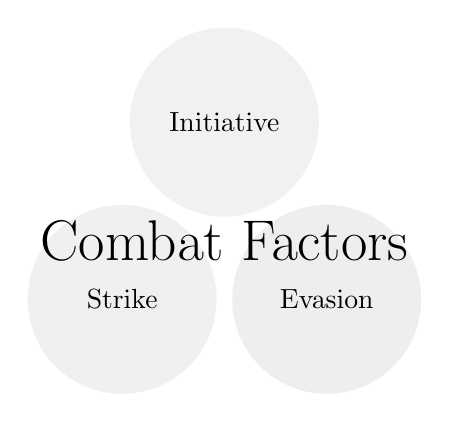
\begin{tikzpicture}
  \begin{scope}[blend group = soft light]
    \fill[gray!11!white]   ( 90:1.5) circle (1.2);
    \fill[gray!12!white] (210:1.5) circle (1.2);
    \fill[gray!13!white]  (330:1.5) circle (1.2);
  \end{scope}
  \node at ( 90:1.5)    {Initiative};
  \node at ( 210:1.5)   {Strike};
  \node at ( 330:1.5)   {Evasion};
  \node [font=\huge] {Combat Factors};
\end{tikzpicture}}

%----

	\posterbox{name=initbox,column=1,row=7,span=3.7,rowspan=1.1}{\begin{multicols}{2}{\tiny \begin{tabular}{lc}
		{\bf Action} & {\bf Cost} \\\hline
		Draw Weapon & 2 \\
		Guarding & 2 \\
		Light Weapon & 4 \\
		Med. Weapon & 6 \\
		Use Item & 8 \\
		Spell & 3+lv. \\
		
	\end{tabular}}
		{\tiny \begin{tabular}{lc}
		{\textbf Quick Actions} & \\\hline
		Evasion & 2 \\
		Keep Edgy & 2 \\
		Move & 2 \\
		Speak & 2 \\
		\end{tabular}}

	\end{multicols}
}
%----

	\posterbox[adjusted title=Abilities \& Specializations]{name=racial_abilities,column=5,row=7,rowspan=1,span=6}{}

%----
	\posterbox[adjusted title=Armoury]{name=armoury,column=5,row=4,span=6,rowspan=3}{
		\begin{tabular}{p{.2\textwidth}lllll}
			Weapon & Dam. & Init. & Ev. & Wt. & Knack \\
			\\
			
			\writeline & \shortline & \shortline & \shortline &\shortline &  \writeline \\
			\writeline & \shortline & \shortline & \shortline &\shortline &  \writeline \\
			\writeline & \shortline & \shortline & \shortline &\shortline &  \writeline \\
			\writeline & \shortline & \shortline & \shortline &\shortline &  \writeline \\
			\writeline & \shortline & \shortline & \shortline &\shortline &  \writeline \\
			\writeline & \shortline & \shortline & \shortline &\shortline &  \writeline \\
		\end{tabular}	
		\vspace{.3cm}

		\begin{tabular}{lcccc}
			Armour & DR & Weight & Type & Encumbrance \\
			\\
			\writeline & \shortline & \shortline & \shortline & \shortline \\
		\end{tabular}

	}
%----
	\posterbox[adjusted title=Skills]{name=skills,column=8,row=8,span=3.1,rowspan=4.8}{
		\begin{tabular}{lp{0em}p{0em}p{0em}}
			\sskill{Combat*}
			\sskill{Projectiles*}
			& \\
			\skill{Academics*}
			\sskill{Athletics}
			\skill{Beast Ken*}
			\sskill{Crafts*}
			\skill{Deceit}
			\skill{Empathy}
			\skill{Medicine*}
			\skill{Performance*}
			\skill{Larceny}
			\skill{Stealth}
			\sskill{Survival*}
			\skill{Tactics*}
			\skill{Vigilance}
			\skill{\line(1,0){70}}
			\sskill{\line(1,0){70}}



		\end{tabular}
	}

	\posterbox[adjusted title=Spheres]{name=spheres,column=1,row=8,span=3.8,rowspan=2}
	{\vspace{.2cm} \line(1,0){110} \fiveboxes

\vspace{.2cm} \line(1,0){110} \fiveboxes

\vspace{.2cm} \line(1,0){110} \fiveboxes

\vspace{.2cm} \line(1,0){110} \fiveboxes

	}

%----

	\posterbox[adjusted title=Equipment]{name=equipment,column=1,row=10,span=7,rowspan=2.8}{

	\vspace{.4cm}

	\longline	

	\longline	

	\longline	

	\longline	

	\longline	

	\longline	

	\longline	

	CP \weeline SP\weeline GP\weeline 

	Total XP \weeline Remaining XP \weeline}

	\posterbox[adjusted title=Knacks]{name=knacks,column=5,row=8,span=3,rowspan=2}{
		\vspace{.3cm}

		\Split
		\Split
		\Split
		\Split
		\Split
		\Split

	}
\end{tcbposter}

\pagebreak

\begin{tcbposter}[
  coverage = {
      spread,
      %interior style={bottom color=white},
      watermark text={stories \\ companions \\ notes},
      watermark color=black!25!white,
      watermark opacity=0.4
  },
  poster   = {showframe=false,columns=11,rows=12},
  boxes    = {
      enhanced standard jigsaw,sharp corners=downhill,arc=7mm,boxrule=.6mm,
      colback=white,opacityback=0.7,colframe=black,
      title style={left color=black,right color=white},
      fonttitle=\bfseries
   }
]

	\posterbox[adjusted title=Stories]{name=stories,column=1,row=1,rowspan=11,span=11}{

		{\Huge Story Points}

		\vspace{0.5cm}

	\begin{tabular}{p{1em}p{1em}p{1em}p{1em}p{1em}p{1em}p{1em}}

		\Huge\ding{111} & \Huge\ding{111} & \Huge\ding{111} & \Huge\ding{111} & \Huge\ding{111} & \huge\ding{111} & \Large\ding{111} \\

	\end{tabular}

		}
\end{tcbposter}



\end{document}

